\documentclass[hyperref={pdfpagelabels=false}]{beamer}
% beamer already loads hyperref; do NOT load \usepackage{hyperref} again.

\usepackage{ragged2e} % 文字向兩邊對齊
\renewcommand{\raggedright}{\leftskip=0pt \rightskip=0pt plus 0cm}

\usepackage{listings}
\usepackage{lmodern}
\usepackage{fontspec}
\usepackage{xeCJK}
\setCJKmainfont{Noto Sans CJK TC}
%（可選）若你會用到無襯線中文或等寬中文，建議補上：
\setCJKsansfont{Noto Sans CJK TC}
\setCJKmonofont{Noto Sans Mono CJK TC}

\usepackage[english]{babel}
\usepackage{amsmath,amssymb,amsfonts,amsthm}

% hyperref settings (since beamer already loads hyperref)
\hypersetup{
  colorlinks=true,
  urlcolor=blue,
  citecolor=blue,
  pdfborder={0 0 0}
}

\usepackage{accsupp}% http://ctan.org/pkg/accsupp
\newcommand{\emptyaccsupp}[1]{\BeginAccSupp{ActualText={}}#1\EndAccSupp{}}

\usepackage{tikz}
\usetikzlibrary{arrows,decorations.pathmorphing,backgrounds,fit,positioning,shapes.symbols,chains}

\usepackage{booktabs}
\usepackage{threeparttable}
\usepackage{colortbl} 
\usepackage{xcolor}
\usetikzlibrary{tikzmark}

\newcommand{\indep}{\perp\!\!\!\perp}
\newcommand{\nindep}{\not\!\perp\!\!\!\perp}

\beamertemplatefootpagenumber


\usepackage{listings}
%%%%%%%%%%%%%%%%%%%%%%%%%%%%%%%%%%%%%%%%%%%%%%%%%%%%%%%%%%%%%%%%%%%%%%%%%%%%%%
% LaTeX snippet: language and style definition of Stata for listings package.
%                [listings](http://www.ctan.org/pkg/listings) 
%                [Stata](http://www.stata.com/)
%
% Usage:
%     Copy the code into your preamble, or import it by `\include` .
%     then in your doc:
%     \lstinputlisting[style=numbers]{DO-SCRIPT}
%     \lstinputlisting[style=numbers, style=stata-editor]{DO-SCRIPT}
%     \lstinputlisting[style=nonumbers, frame=none]{DO-SCRIPT}
% How it works:
%     - The language is defined by `\lstdefinelanguage{Stata}`
%     - Four styles is defined by `\lstdefinestyle{STYLE-NAME}`, 
%       they are: numbers and no numbers, plain(black and white) and colorful
%       (colored roughly like stata editor.)
% Tips:
%     - Generally you only need to set your default in the last part,
%       that is, code inside of `\lstset`.
%     - Add more keywords(I can not list all of them) in the `\lstset` part.
%     - Do NOT leave any blank lines in commands
%       (`\lstddefinelanguage', `\lstdefinestyle` and `\lstset`)
%
% update: 2014-04-16
% version: 0.1
% author: kongs
% licence: MIT
% url: https://gist.github.com/kongs-sublime/10862838
%
% TODO: 
%       - finish keyword list.
%       - precise colors that match stata editor?
%       - make it flexible(fonts and style)
%
%%%%%%%%%%%%%%%%%%%%%%%%%%%%%%%%%%%%%%%%%%%%%%%%%%%%%%%%%%%%%%%%%%%%%%%%%%%%%%


% langugae defination
\lstdefinelanguage{Stata}{
	% Left for users to add missing commands,
	% with possibility of choosing different style.
	morekeywords=,
	% Popular add-on commands
	morekeywords=[2]{cntrade, chinafin, 
		wbopendata, spmap,
	},
	% System commands
	morekeywords=[3]{regress, summarize, 
		display,
	},
	% Keywords
	morekeywords=[4]{forvalues, if, foreach, set},
	% Built-in functions
	morekeywords=[5]{rnormal, runiform},
	morecomment=[l]{//},
	% morecomment=[l]{*},  // `*` maybe used as multiply operator. So use `//` as line comment.
	morecomment=[s]{/*}{*/},
	% morecomment=[s]{,}{//},
	% The following is used by macros, like `lags'.
	morecomment=[n][keywordstyle9]{`}{'},
	morestring=[b]",
	sensitive=true,
}

\lstdefinestyle{numbers}{
	numbers=left, 
	stepnumber=1, 
	numberstyle=\tiny\emptyaccsupp,
	xleftmargin=2em,
}

\lstdefinestyle{nonumbers}{
	numbers=none,
}

\lstdefinestyle{stata-plain}{
	language=Stata,
	basicstyle=\footnotesize\ttfamily,
}

\lstdefinestyle{stata-editor}{
	language=Stata,
	basicstyle=\footnotesize\ttfamily,  
	keywordstyle={\color{NavyBlue}},  
	keywordstyle=[2]{\color{NavyBlue}},
	keywordstyle=[3]{\color{NavyBlue}},
	keywordstyle=[4]{\color{NavyBlue}},
	keywordstyle=[5]{\color{Blue}},
	keywordstyle=[9]{\color{TealBlue}},
	stringstyle=\color{Maroon},
	commentstyle=\color{OliveGreen},
}

\lstset{
	language=Stata,
	style=stata-plain,
	% style=stata-editor,
	style=numbers,
	showstringspaces=false,
	breaklines,
	frame=single,
	% To add missing commands
	% morekeywords={xtreg, xtunitroot},
}




\title[]  
{Matching Methods}

%\subtitle
%{免除部分負擔對幼兒醫療利用與健康的影響:斷點迴歸分析}

%\author 
 %{Tzu-Ting Yang\inst{1} \and Hsing-Wen Han\inst{2} \and Hsien-Ming Lien\inst{3}}

%\institute[short]{\inst{1} Academia Sinica \and \inst{2} Tamkang University \and \inst{3} National Chengchi University}


%\author 
 %{Prof. Tzu-Ting Yang}

%\institute{Institute of Economics, Academia Sinica  \\ Econ, NTU}
%\institute{Institute of Economics, Academia Sinica  \\ IMES/IDAS, NCCU}
%\institute{Institute of Economics, Academia Sinica}


\author 
{Prof. Tzu-Ting Yang  \\ 楊子霆}

%\institute{Institute of Economics, Academia Sinica  \\ Econ, NTU}
\institute{Institute of Economics, Academia Sinica  \\ 中央研究院經濟研究所}
%\institute{Institute of Economics, Academia Sinica  \\ Econ, NTU}
%\institute{Institute of Economics, Academia Sinica  \\ IMES/IDAS, NCCU}

%\author 
%{楊子霆 \\ 中研院經濟所}

%\institute 
%{中正大學國際經濟專題研討}




\date
{\today}



% \usetheme{CambridgeUS}
% %\usecolortheme{seahorse}
% \setbeamertemplate{footline}{%
% 	\hfill\usebeamercolor[fg]{page number in head/foot}%
% 	\usebeamerfont{page number in head/foot}%
% 	\insertframenumber\,/\,\inserttotalframenumber\hspace{1em}\vspace{2pt}%
% }

\usetheme{Boadilla}
%\useinnertheme{rectangles}

%\usetheme{CambridgeUS}
\usecolortheme{seahorse}
\setbeamertemplate{footline}{%
	\hfill\usebeamercolor[fg]{page number in head/foot}%
	\usebeamerfont{page number in head/foot}%
	\insertframenumber\,/\,\inserttotalframenumber\hspace{1em}\vspace{2pt}%
}


% \usepackage{beamerthemeshadow}
% %\usecolortheme{seahorse}
% \setbeamertemplate{footline}{%
% 	\hfill\usebeamercolor[fg]{page number in head/foot}%
% 	\usebeamerfont{page number in head/foot}%
% 	\insertframenumber\,/\,\inserttotalframenumber\hspace{1em}\vspace{2pt}%
% }



%\usepackage{beamerthemeshadow}
\beamersetuncovermixins{\opaqueness<1>{25}}{\opaqueness<2->{15}}

\begin{document}


\begin{frame}{}
 \titlepage
\end{frame}




%Causal inference requires the estimation of the unconditional means of the outcomes for each treatment level. We only observe the outcome of each subject conditional on the received treatment regardless of whether the data are observational or experimental. For experimental data, random assignment of the treatment guarantees that the treatment is independent of the outcome; so averages of the outcomes conditional on observed treatment estimate the unconditional means of interest. For observational data, we model the treatment assignment process. If our model is correct, the treatment assignment process is considered as good as random conditional on the covariates in our model.


\begin{frame}{Observational Studies}
	\begin{itemize} 
		\item Randomized Controlled Trial (RCT) is called the ``gold standard" for causal inference 
		\vspace{0.3cm}
			\begin{itemize} 
		\item In a RCT, researcher can assign treatments randomly to the individuals
		\vspace{0.3cm}
		\item Therefore, \textbf{treatment status is unrelated to any observed and unobserved confounders}
					\begin{itemize} 
			\vspace{0.3cm}
		\item Treatment and control group should be similar in all characteristics
					\vspace{0.3cm}
		\item Thus, we can use the observed outcomes of control group to approximate the counterfactual outcomes of treatment group		
					\end{itemize}
			\end{itemize}
		
	\end{itemize}
\end{frame}


\begin{frame}{Observational Studies}
	\begin{itemize} 
		
		\item But implementing a randomized experiment in social science is very expensive and sometimes has ethical issues
		\vspace{0.3cm}
		\item In social science, many empirical studies use \textbf{non-experimental data} 
		\vspace{0.3cm}
			\begin{itemize} 
	\item It means researchers \textbf{can NOT assign treatment	}
			\end{itemize}
				\vspace{0.3cm}
		\item We call this type of empirical researches as \textbf{observational studies}
		
	\end{itemize}
\end{frame}


\begin{frame}{Observational Studies}
	\begin{itemize} 
	
		\item We want to \textbf{design} observational studies that \textbf{approximate experiments}:
		\begin{itemize}
			\vspace{0.3cm}
			\item ``The planner of an observational study should always ask himself: How would the study be conducted if it were possible to do it by controlled experimentation" (Cochran 1965)
		\end{itemize}
				\vspace{0.3cm}
	\item How to do that?
					\vspace{0.3cm}
				\begin{itemize}			
	\item Need to directly control for the observed variables
		\vspace{0.3cm}
	\item Use indirect methods to adjust for unobserved variables
	\vspace{0.3cm}
	\item Make ``other thing equal" in observed and unobserved variables
		\end{itemize}
	\end{itemize}
\end{frame}




\title[]  
{Matching Methods: Main Idea}


\author 
{}

%\institute{Institute of Economics, Academia Sinica  \\ Econ, NTU}
%\institute{Institute of Economics, Academia Sinica  \\ IMES/IDAS, NCCU}
\institute{}

%\author 
%{楊子霆 \\ 中研院經濟所}

%\institute 
%{中正大學國際經濟專題研討}




\date
{}


\begin{frame}{}
\titlepage
\end{frame}




\begin{frame}{Main Idea of Matching}
	\begin{itemize} 
		
		\item Assume all confounding factors are \textbf{observable} to researchers
				\vspace{0.2cm}

		\item Matching is a way to eliminate selection bias 
		
							\begin{itemize} 
												\vspace{0.2cm}
		%\item By controlling for observable covariates
		%\vspace{0.2cm}
		\item By constructing a control group with the same observable characteristics as the treatment group
			\end{itemize}
				\vspace{0.2cm}
			\item This can be accomplished by \textbf{matching} treated and untreated units with the same observable characteristics.
		
		
	\end{itemize}
\end{frame}




\begin{frame}{Main Idea of Matching}
	\begin{itemize}
		
		\item \textbf{Example:} 
				\vspace{0.2cm}
			\begin{itemize}
		\item We want to estimate the causal effect of job training program on worker's earnings
		\vspace{0.2cm}

		\item Suppose \textbf{age} is the only confounding factors that affect both earnings and job training decision
		%\item If all matches are perfect (no matching discrepancies) the resulting estimator is identical to the subclassification estimator.
					\end{itemize}
	\end{itemize}
\end{frame}


\begin{frame}{Matching: A Numerical Example}
	%% 1
	\begin{center}
\scalebox{0.80}{
			\begin{threeparttable}
				\centering\footnotesize
				\begin{tabular}{@{} ccrccrccr @{}}
					\multicolumn{3}{c}{Trainees} & \multicolumn{3}{c}{Non-Trainees} & \multicolumn{3}{c}{\textcolor{white}{Matched Sample}}\\
					\cmidrule(l){1-3}  \cmidrule(l){4-6} %\cmidrule(l){7-9} 
					unit   & age   & earnings   & unit   & age   & earnings  & \textcolor{white}{unit}   & \textcolor{white}{age}   & \textcolor{white}{earnings} \\
					1 & 28 & 17700 &  1 & 43 & 20900 &    &  &   \\
					2 & 34 & 10200 &  2 & 50 & 31000 &    &  &   \\ 
					3 & 29 & 14400 &  3 & 30 & 21000 &    &  &   \\ 
					4 & 25 & 20800 &  4 & 27 & 9300  &    &  &   \\  
					5 & 29 & 6100  &  5 & 54 & 41100 &    &  &   \\
					6 & 23 & 28600 &  6 & 48 & 29800 &    &  &   \\
					7 & 33 & 21900 &  7 & 39 & 42000 &    &  &   \\
					8 & 27 & 28800 &  8 & 28 & 8800  &    &  &   \\  
					9 & 31 & 20300 &  9 & 24 & 25500 &    &  &   \\  
					10 & 26 & 28100 & 10 & 33 & 15500 & {\color{white}11,13}   &  &   \\
					11 & 25 & 9400  & 11 & 26 & 400   &    &  &   \\
					12 & 27 & 14300 & 12 & 31 & 26600 &    &  &   \\
					13 & 29 & 12500 & 13 & 26 & 16500 &    &  &   \\
					14 & 24 & 19700 & 14 & 34 & 24200 &    &  &   \\
					15 & 25 & 10100 & 15 & 25 & 23300 &    &  &   \\
					16 & 43 & 10700 & 16 & 24 & 9700  &    &  &   \\ 
					17 & 28 & 11500 & 17 & 29 & 6200  &    &  &   \\ 
					18 & 27 & 10700 & 18 & 35 & 30200 &    &  &   \\
					19 & 28 & 16300 & 19 & 32 & 17800 &    &  &   \\ 
					&    &       & 20 & 23 & 9500  &    &  &   \\
					&    &       & 21 & 32 & 25900 &    &  &   \\ 
					\cmidrule(l){1-3}  \cmidrule(l){4-6} %\cmidrule(l){7-9} 
					Avg: & 28.5 & 16426 & Avg: & 33 & 20724 & {\color{white}Avg:} & {\color{white}28.5} &  \\
				\end{tabular}
		\end{threeparttable}}
	\end{center}
\end{frame}


\begin{frame}{Matching: A Numerical Example}
	%% 2
	\begin{center}
\scalebox{0.80}{
			\begin{threeparttable}
				\centering\footnotesize
				\begin{tabular}{@{} ccrccrccr @{}}
					\multicolumn{3}{c}{Trainees} & \multicolumn{3}{c}{Non-Trainees} & \multicolumn{3}{c}{Matched Sample}\\
					\cmidrule(l){1-3}  \cmidrule(l){4-6} \cmidrule(l){7-9} 
					unit   & age   & earnings   & unit   & age   & earnings  & unit  & age   & earnings \\
					1 & 28 & 17700 &  1 & 43 & 20900 &    &  &   \\
					2 & 34 & 10200 &  2 & 50 & 31000 &    &  &   \\ 
					3 & 29 & 14400 &  3 & 30 & 21000 &    &  &   \\ 
					4 & 25 & 20800 &  4 & 27 & 9300  &    &  &   \\  
					5 & 29 & 6100  &  5 & 54 & 41100 &    &  &   \\
					6 & 23 & 28600 &  6 & 48 & 29800 &    &  &   \\
					7 & 33 & 21900 &  7 & 39 & 42000 &    &  &   \\
					8 & 27 & 28800 &  8 & 28 & 8800  &    &  &   \\  
					9 & 31 & 20300 &  9 & 24 & 25500 &    &  &   \\  
					10 & 26 & 28100 & 10 & 33 & 15500 & {\color{white}11,13}   &  &   \\
					11 & 25 & 9400  & 11 & 26 & 400   &    &  &   \\
					12 & 27 & 14300 & 12 & 31 & 26600 &    &  &   \\
					13 & 29 & 12500 & 13 & 26 & 16500 &    &  &   \\
					14 & 24 & 19700 & 14 & 34 & 24200 &    &  &   \\
					15 & 25 & 10100 & 15 & 25 & 23300 &    &  &   \\
					16 & 43 & 10700 & 16 & 24 & 9700  &    &  &   \\ 
					17 & 28 & 11500 & 17 & 29 & 6200  &    &  &   \\ 
					18 & 27 & 10700 & 18 & 35 & 30200 &    &  &   \\
					19 & 28 & 16300 & 19 & 32 & 17800 &    &  &   \\ 
					&    &       & 20 & 23 & 9500  &    &  &   \\
					&    &       & 21 & 32 & 25900 &    &  &   \\ 
					\cmidrule(l){1-3}  \cmidrule(l){4-6} \cmidrule(l){7-9} 
					Avg: & 28.5 & 16426 & Avg: & 33 & 20724 & Avg: & {\color{white}28.5} &  \\
				\end{tabular}
		\end{threeparttable}}
	\end{center}
\end{frame}


\begin{frame}{Matching: A Numerical Example}
	%% 3
	\begin{center}
\scalebox{0.80}{
			\begin{threeparttable}
				\centering\footnotesize
				\begin{tabular}{@{} ccrccrccr @{}}
					\multicolumn{3}{c}{Trainees} & \multicolumn{3}{c}{Non-Trainees} & \multicolumn{3}{c}{Matched Sample}\\
					\cmidrule(l){1-3}  \cmidrule(l){4-6} \cmidrule(l){7-9} 
					unit   & age   & earnings   & unit   & age   & earnings  & unit  & age   & earnings \\
					{\color{red}1} & {\color{red}28} &  {\color{red}17700} &  1 & 43 & 20900 &    &  &   \\
					2 & 34 & 10200 &  2 & 50 & 31000 &    &  &   \\ 
					3 & 29 & 14400 &  3 & 30 & 21000 &    &  &   \\ 
					4 & 25 & 20800 &  4 & 27 & 9300  &    &  &   \\  
					5 & 29 & 6100  &  5 & 54 & 41100 &    &  &   \\
					6 & 23 & 28600 &  6 & 48 & 29800 &    &  &   \\
					7 & 33 & 21900 &  7 & 39 & 42000 &    &  &   \\
					8 & 27 & 28800 &  8 & 28 & 8800  &    &  &   \\  
					9 & 31 & 20300 &  9 & 24 & 25500 &    &  &   \\  
					10 & 26 & 28100 & 10 & 33 & 15500 & {\color{white}11,13}   &  &   \\
					11 & 25 & 9400  & 11 & 26 & 400   &    &  &   \\
					12 & 27 & 14300 & 12 & 31 & 26600 &    &  &   \\
					13 & 29 & 12500 & 13 & 26 & 16500 &    &  &   \\
					14 & 24 & 19700 & 14 & 34 & 24200 &    &  &   \\
					15 & 25 & 10100 & 15 & 25 & 23300 &    &  &   \\
					16 & 43 & 10700 & 16 & 24 & 9700  &    &  &   \\ 
					17 & 28 & 11500 & 17 & 29 & 6200  &    &  &   \\ 
					18 & 27 & 10700 & 18 & 35 & 30200 &    &  &   \\
					19 & 28 & 16300 & 19 & 32 & 17800 &    &  &   \\ 
					&    &       & 20 & 23 & 9500  &    &  &   \\
					&    &       & 21 & 32 & 25900 &    &  &   \\ 
					\cmidrule(l){1-3}  \cmidrule(l){4-6} \cmidrule(l){7-9} 
					Avg: & 28.5 & 16426 & Avg: & 33 & 20724 & Avg: & {\color{white}28.5} &  \\
				\end{tabular}
		\end{threeparttable}}
	\end{center}
\end{frame}


\begin{frame}{Matching: A Numerical Example}
	%% 4
	\begin{center}
\scalebox{0.80}{
			\begin{threeparttable}
				\centering\footnotesize
				\begin{tabular}{@{} ccrccrccr @{}}
					\multicolumn{3}{c}{Trainees} & \multicolumn{3}{c}{Non-Trainees} & \multicolumn{3}{c}{Matched Sample}\\
					\cmidrule(l){1-3}  \cmidrule(l){4-6} \cmidrule(l){7-9} 
					unit   & age   & earnings   & unit   & age   & earnings  & unit  & age   & earnings \\
					{\color{red}1} & {\color{red}28} &  {\color{red}17700} &  1 & 43 & 20900 &    &  &   \\
					2 & 34 & 10200 &  2 & 50 & 31000 &    &  &   \\ 
					3 & 29 & 14400 &  3 & 30 & 21000 &    &  &   \\ 
					4 & 25 & 20800 &  4 & 27 & 9300  &    &  &   \\  
					5 & 29 & 6100  &  5 & 54 & 41100 &    &  &   \\
					6 & 23 & 28600 &  6 & 48 & 29800 &    &  &   \\
					7 & 33 & 21900 &  7 & 39 & 42000 &    &  &   \\
					8 & 27 & 28800 &  {\color{red}8} & {\color{red}28} & {\color{red}8800}  &    &  &   \\  
					9 & 31 & 20300 &  9 & 24 & 25500 &    &  &   \\  
					10 & 26 & 28100 & 10 & 33 & 15500 & {\color{white}11,13}   &  &   \\
					11 & 25 & 9400  & 11 & 26 & 400   &    &  &   \\
					12 & 27 & 14300 & 12 & 31 & 26600 &    &  &   \\
					13 & 29 & 12500 & 13 & 26 & 16500 &    &  &   \\
					14 & 24 & 19700 & 14 & 34 & 24200 &    &  &   \\
					15 & 25 & 10100 & 15 & 25 & 23300 &    &  &   \\
					16 & 43 & 10700 & 16 & 24 & 9700  &    &  &   \\ 
					17 & 28 & 11500 & 17 & 29 & 6200  &    &  &   \\ 
					18 & 27 & 10700 & 18 & 35 & 30200 &    &  &   \\
					19 & 28 & 16300 & 19 & 32 & 17800 &    &  &   \\ 
					&    &       & 20 & 23 & 9500  &    &  &   \\
					&    &       & 21 & 32 & 25900 &    &  &   \\ 
					\cmidrule(l){1-3}  \cmidrule(l){4-6} \cmidrule(l){7-9} 
					Avg: & 28.5 & 16426 & Avg: & 33 & 20724 & Avg: & {\color{white}28.5} &  \\
				\end{tabular}
		\end{threeparttable}}
	\end{center}
\end{frame}


\begin{frame}{Matching: A Numerical Example}
	%% 5
	\begin{center}
\scalebox{0.80}{
			\begin{threeparttable}
				\centering\footnotesize
				\begin{tabular}{@{} ccrccrccr @{}}
					\multicolumn{3}{c}{Trainees} & \multicolumn{3}{c}{Non-Trainees} & \multicolumn{3}{c}{Matched Sample}\\
					\cmidrule(l){1-3}  \cmidrule(l){4-6} \cmidrule(l){7-9} 
					unit   & age   & earnings   & unit   & age   & earnings  & unit  & age   & earnings \\
					{\color{red}1} & {\color{red}28} &  {\color{red}17700} &  1 & 43 & 20900 &  {\color{red}8}  & {\color{red}28} & {\color{red}8800}  \\
					2 & 34 & 10200 &  2 & 50 & 31000 &    &  &   \\ 
					3 & 29 & 14400 &  3 & 30 & 21000 &    &  &   \\ 
					4 & 25 & 20800 &  4 & 27 & 9300  &    &  &   \\  
					5 & 29 & 6100  &  5 & 54 & 41100 &    &  &   \\
					6 & 23 & 28600 &  6 & 48 & 29800 &    &  &   \\
					7 & 33 & 21900 &  7 & 39 & 42000 &    &  &   \\
					8 & 27 & 28800 &  {\color{red}8} & {\color{red}28} & {\color{red}8800}  &    &  &   \\  
					9 & 31 & 20300 &  9 & 24 & 25500 &    &  &   \\  
					10 & 26 & 28100 & 10 & 33 & 15500 & {\color{white}11,13}   &  &   \\
					11 & 25 & 9400  & 11 & 26 & 400   &    &  &   \\
					12 & 27 & 14300 & 12 & 31 & 26600 &    &  &   \\
					13 & 29 & 12500 & 13 & 26 & 16500 &    &  &   \\
					14 & 24 & 19700 & 14 & 34 & 24200 &    &  &   \\
					15 & 25 & 10100 & 15 & 25 & 23300 &    &  &   \\
					16 & 43 & 10700 & 16 & 24 & 9700  &    &  &   \\ 
					17 & 28 & 11500 & 17 & 29 & 6200  &    &  &   \\ 
					18 & 27 & 10700 & 18 & 35 & 30200 &    &  &   \\
					19 & 28 & 16300 & 19 & 32 & 17800 &    &  &   \\ 
					&    &       & 20 & 23 & 9500  &    &  &   \\
					&    &       & 21 & 32 & 25900 &    &  &   \\ 
					\cmidrule(l){1-3}  \cmidrule(l){4-6} \cmidrule(l){7-9} 
					Avg: & 28.5 & 16426 & Avg: & 33 & 20724 & Avg: & {\color{white}28.5} &  \\
				\end{tabular}
		\end{threeparttable}}
	\end{center}
\end{frame}


\begin{frame}{Matching: A Numerical Example}
	%% 6
	\begin{center}
\scalebox{0.80}{
			\begin{threeparttable}
				\centering\footnotesize
				\begin{tabular}{@{} ccrccrccr @{}}
					\multicolumn{3}{c}{Trainees} & \multicolumn{3}{c}{Non-Trainees} & \multicolumn{3}{c}{Matched Sample}\\
					\cmidrule(l){1-3}  \cmidrule(l){4-6} \cmidrule(l){7-9} 
					unit   & age   & earnings   & unit   & age   & earnings  & unit  & age   & earnings \\
					1 & 28 & 17700 &  1 & 43 & 20900 & 8  & 28 & 8800  \\
					{\color{red}2} & {\color{red}34} & {\color{red}10200} &  2 & 50 & 31000 & {\color{red}14}   & {\color{red}34} & {\color{red}24200}  \\ 
					3 & 29 & 14400 &  3 & 30 & 21000 &    &  &   \\ 
					4 & 25 & 20800 &  4 & 27 & 9300  &    &  &   \\  
					5 & 29 & 6100  &  5 & 54 & 41100 &    &  &   \\
					6 & 23 & 28600 &  6 & 48 & 29800 &    &  &   \\
					7 & 33 & 21900 &  7 & 39 & 42000 &    &  &   \\
					8 & 27 & 28800 &  8 & 28 & 8800  &    &  &   \\  
					9 & 31 & 20300 &  9 & 24 & 25500 &    &  &   \\  
					10 & 26 & 28100 & 10 & 33 & 15500 & {\color{white}11,13}   &  &   \\
					11 & 25 & 9400  & 11 & 26 & 400   &    &  &   \\
					12 & 27 & 14300 & 12 & 31 & 26600 &    &  &   \\
					13 & 29 & 12500 & 13 & 26 & 16500 &    &  &   \\
					14 & 24 & 19700 & {\color{red}14} & {\color{red}34} & {\color{red}24200} &    &  &   \\
					15 & 25 & 10100 & 15 & 25 & 23300 &    &  &   \\
					16 & 43 & 10700 & 16 & 24 & 9700  &    &  &   \\ 
					17 & 28 & 11500 & 17 & 29 & 6200  &    &  &   \\ 
					18 & 27 & 10700 & 18 & 35 & 30200 &    &  &   \\
					19 & 28 & 16300 & 19 & 32 & 17800 &    &  &   \\ 
					&    &       & 20 & 23 & 9500  &    &  &   \\
					&    &       & 21 & 32 & 25900 &    &  &   \\ 
					\cmidrule(l){1-3}  \cmidrule(l){4-6} \cmidrule(l){7-9} 
					Avg: & 28.5 & 16426 & Avg: & 33 & 20724 & Avg: & {\color{white}28.5} &  \\
				\end{tabular}
		\end{threeparttable}}
	\end{center}
\end{frame}


\begin{frame}{Matching: A Numerical Example}
	%% 7
	\begin{center}
\scalebox{0.80}{
			\begin{threeparttable}
				\centering\footnotesize
				\begin{tabular}{@{} ccrccrccr @{}}
					\multicolumn{3}{c}{Trainees} & \multicolumn{3}{c}{Non-Trainees} & \multicolumn{3}{c}{Matched Sample}\\
					\cmidrule(l){1-3}  \cmidrule(l){4-6} \cmidrule(l){7-9} 
					unit   & age   & earnings   & unit   & age   & earnings  & unit  & age   & earnings \\
					1 & 28 & 17700 &  1 & 43 & 20900 &  8 & 28 & 8800   \\
					2 & 34 & 10200 &  2 & 50 & 31000 & 14 & 34 & 24200  \\ 
					{\color{red}3} & {\color{red}29} & {\color{red}14400} &  3 & 30 & 21000 & {\color{red}17}   & {\color{red}29} & {\color{red}6200}  \\ 
					4 & 25 & 20800 &  4 & 27 & 9300  &    &  &   \\  
					5 & 29 & 6100  &  5 & 54 & 41100 &    &  &   \\
					6 & 23 & 28600 &  6 & 48 & 29800 &    &  &   \\
					7 & 33 & 21900 &  7 & 39 & 42000 &    &  &   \\
					8 & 27 & 28800 &  8 & 28 & 8800  &    &  &   \\  
					9 & 31 & 20300 &  9 & 24 & 25500 &    &  &   \\  
					10 & 26 & 28100 & 10 & 33 & 15500 & {\color{white}11,13}   &  &   \\
					11 & 25 & 9400  & 11 & 26 & 400   &    &  &   \\
					12 & 27 & 14300 & 12 & 31 & 26600 &    &  &   \\
					13 & 29 & 12500 & 13 & 26 & 16500 &    &  &   \\
					14 & 24 & 19700 & 14 & 34 & 24200 &    &  &   \\
					15 & 25 & 10100 & 15 & 25 & 23300 &    &  &   \\
					16 & 43 & 10700 & 16 & 24 & 9700  &    &  &   \\ 
					17 & 28 & 11500 & {\color{red}17} & {\color{red}29} & {\color{red}6200}  &    &  &   \\ 
					18 & 27 & 10700 & 18 & 35 & 30200 &    &  &   \\
					19 & 28 & 16300 & 19 & 32 & 17800 &    &  &   \\ 
					&    &       & 20 & 23 & 9500  &    &  &   \\
					&    &       & 21 & 32 & 25900 &    &  &   \\ 
					\cmidrule(l){1-3}  \cmidrule(l){4-6} \cmidrule(l){7-9} 
					Avg: & 28.5 & 16426 & Avg: & 33 & 20724 & Avg: & {\color{white}28.5} &  \\
				\end{tabular}
		\end{threeparttable}}
	\end{center}
\end{frame}


\begin{frame}{Matching: A Numerical Example}
	%% 8
	\begin{center}
\scalebox{0.80}{
			\begin{threeparttable}
				\centering\footnotesize
				\begin{tabular}{@{} ccrccrccr @{}}
					\multicolumn{3}{c}{Trainees} & \multicolumn{3}{c}{Non-Trainees} & \multicolumn{3}{c}{Matched Sample}\\
					\cmidrule(l){1-3}  \cmidrule(l){4-6} \cmidrule(l){7-9} 
					unit   & age   & earnings   & unit   & age   & earnings  & unit  & age   & earnings \\
					1 & 28 & 17700 &  1 & 43 & 20900 &  8 & 28 & 8800   \\
					2 & 34 & 10200 &  2 & 50 & 31000 & 14 & 34 & 24200  \\ 
					3 & 29 & 14400 &  3 & 30 & 21000 & 17 & 29 & 6200   \\ 
					{\color{red}4} & {\color{red}25} & {\color{red}20800} &  4 & 27 & 9300  & {\color{red}15}   & {\color{red}25} & {\color{red}23300}  \\  
					5 & 29 & 6100  &  5 & 54 & 41100 &    &  &   \\
					6 & 23 & 28600 &  6 & 48 & 29800 &    &  &   \\
					7 & 33 & 21900 &  7 & 39 & 42000 &    &  &   \\
					8 & 27 & 28800 &  8 & 28 & 8800  &    &  &   \\  
					9 & 31 & 20300 &  9 & 24 & 25500 &    &  &   \\  
					10 & 26 & 28100 & 10 & 33 & 15500 & {\color{white}11,13}   &  &   \\
					11 & 25 & 9400  & 11 & 26 & 400   &    &  &   \\
					12 & 27 & 14300 & 12 & 31 & 26600 &    &  &   \\
					13 & 29 & 12500 & 13 & 26 & 16500 &    &  &   \\
					14 & 24 & 19700 & 14 & 34 & 24200 &    &  &   \\
					15 & 25 & 10100 & {\color{red}15} & {\color{red}25} & {\color{red}23300} &    &  &   \\
					16 & 43 & 10700 & 16 & 24 & 9700  &    &  &   \\ 
					17 & 28 & 11500 & 17 & 29 & 6200  &    &  &   \\ 
					18 & 27 & 10700 & 18 & 35 & 30200 &    &  &   \\
					19 & 28 & 16300 & 19 & 32 & 17800 &    &  &   \\ 
					&    &       & 20 & 23 & 9500  &    &  &   \\
					&    &       & 21 & 32 & 25900 &    &  &   \\ 
					\cmidrule(l){1-3}  \cmidrule(l){4-6} \cmidrule(l){7-9} 
					Avg: & 28.5 & 16426 & Avg: & 33 & 20724 & Avg: & {\color{white}28.5} &  \\
				\end{tabular}
		\end{threeparttable}}
	\end{center}
\end{frame}


\begin{frame}{Matching: A Numerical Example}
	%% 9
	\begin{center}
\scalebox{0.80}{
			\begin{threeparttable}
				\centering\footnotesize
				\begin{tabular}{@{} ccrccrccr @{}}
					\multicolumn{3}{c}{Trainees} & \multicolumn{3}{c}{Non-Trainees} & \multicolumn{3}{c}{Matched Sample}\\
					\cmidrule(l){1-3}  \cmidrule(l){4-6} \cmidrule(l){7-9} 
					unit   & age   & earnings   & unit   & age   & earnings  & unit  & age   & earnings \\
					1 & 28 & 17700 &  1 & 43 & 20900 &  8 & 28 & 8800   \\
					2 & 34 & 10200 &  2 & 50 & 31000 & 14 & 34 & 24200  \\ 
					3 & 29 & 14400 &  3 & 30 & 21000 & 17 & 29 & 6200   \\ 
					4 & 25 & 20800 &  4 & 27 & 9300  & 15 & 25 & 23300  \\  
					{\color{red}5} & {\color{red}29} & {\color{red}6100}  &  5 & 54 & 41100 & {\color{red}17}   & {\color{red}29} & {\color{red}6200}  \\
					6 & 23 & 28600 &  6 & 48 & 29800 &    &  &   \\
					7 & 33 & 21900 &  7 & 39 & 42000 &    &  &   \\
					8 & 27 & 28800 &  8 & 28 & 8800  &    &  &   \\  
					9 & 31 & 20300 &  9 & 24 & 25500 &    &  &   \\  
					10 & 26 & 28100 & 10 & 33 & 15500 & {\color{white}11,13}   &  &   \\
					11 & 25 & 9400  & 11 & 26 & 400   &    &  &   \\
					12 & 27 & 14300 & 12 & 31 & 26600 &    &  &   \\
					13 & 29 & 12500 & 13 & 26 & 16500 &    &  &   \\
					14 & 24 & 19700 & 14 & 34 & 24200 &    &  &   \\
					15 & 25 & 10100 & 15 & 25 & 23300 &    &  &   \\
					16 & 43 & 10700 & 16 & 24 & 9700  &    &  &   \\ 
					17 & 28 & 11500 & {\color{red}17} & {\color{red}29} & {\color{red}6200}  &    &  &   \\ 
					18 & 27 & 10700 & 18 & 35 & 30200 &    &  &   \\
					19 & 28 & 16300 & 19 & 32 & 17800 &    &  &   \\ 
					&    &       & 20 & 23 & 9500  &    &  &   \\
					&    &       & 21 & 32 & 25900 &    &  &   \\ 
					\cmidrule(l){1-3}  \cmidrule(l){4-6} \cmidrule(l){7-9} 
					Avg: & 28.5 & 16426 & Avg: & 33 & 20724 & Avg: & {\color{white}28.5} &  \\
				\end{tabular}
		\end{threeparttable}}
	\end{center}
\end{frame}


\begin{frame}{Matching: A Numerical Example}
	%% 10
	\begin{center}
\scalebox{0.80}{
			\begin{threeparttable}
				\centering\footnotesize
				\begin{tabular}{@{} ccrccrccr @{}}
					\multicolumn{3}{c}{Trainees} & \multicolumn{3}{c}{Non-Trainees} & \multicolumn{3}{c}{Matched Sample}\\
					\cmidrule(l){1-3}  \cmidrule(l){4-6} \cmidrule(l){7-9} 
					unit   & age   & earnings   & unit   & age   & earnings  & unit  & age   & earnings \\
					1 & 28 & 17700 &  1 & 43 & 20900 &  8 & 28 & 8800   \\
					2 & 34 & 10200 &  2 & 50 & 31000 & 14 & 34 & 24200  \\ 
					3 & 29 & 14400 &  3 & 30 & 21000 & 17 & 29 & 6200   \\ 
					4 & 25 & 20800 &  4 & 27 & 9300  & 15 & 25 & 23300  \\  
					5 & 29 & 6100  &  5 & 54 & 41100 & 17 & 29 & 6200  \\
					{\color{red}6} & {\color{red}23} & {\color{red}28600} &  6 & 48 & 29800 & {\color{red}20}   & {\color{red}23} & {\color{red}9500}  \\
					7 & 33 & 21900 &  7 & 39 & 42000 &    &  &   \\
					8 & 27 & 28800 &  8 & 28 & 8800  &    &  &   \\  
					9 & 31 & 20300 &  9 & 24 & 25500 &    &  &   \\  
					10 & 26 & 28100 & 10 & 33 & 15500 & {\color{white}11,13}   &  &   \\
					11 & 25 & 9400  & 11 & 26 & 400   &    &  &   \\
					12 & 27 & 14300 & 12 & 31 & 26600 &    &  &   \\
					13 & 29 & 12500 & 13 & 26 & 16500 &    &  &   \\
					14 & 24 & 19700 & 14 & 34 & 24200 &    &  &   \\
					15 & 25 & 10100 & 15 & 25 & 23300 &    &  &   \\
					16 & 43 & 10700 & 16 & 24 & 9700  &    &  &   \\ 
					17 & 28 & 11500 & 17 & 29 & 6200  &    &  &   \\ 
					18 & 27 & 10700 & 18 & 35 & 30200 &    &  &   \\
					19 & 28 & 16300 & 19 & 32 & 17800 &    &  &   \\ 
					&    &       & {\color{red}20} & {\color{red}23} & {\color{red}9500}  &    &  &   \\
					&    &       & 21 & 32 & 25900 &    &  &   \\ 
					\cmidrule(l){1-3}  \cmidrule(l){4-6} \cmidrule(l){7-9} 
					Avg: & 28.5 & 16426 & Avg: & 33 & 20724 & Avg: & {\color{white}28.5} &  \\
				\end{tabular}
		\end{threeparttable}}
	\end{center}
\end{frame}


\begin{frame}{Matching: A Numerical Example}
	%% 11
	\begin{center}
\scalebox{0.80}{
			\begin{threeparttable}
				\centering\footnotesize
				\begin{tabular}{@{} ccrccrccr @{}}
					\multicolumn{3}{c}{Trainees} & \multicolumn{3}{c}{Non-Trainees} & \multicolumn{3}{c}{Matched Sample}\\
					\cmidrule(l){1-3}  \cmidrule(l){4-6} \cmidrule(l){7-9} 
					unit   & age   & earnings   & unit   & age   & earnings  & unit  & age   & earnings \\
					1 & 28 & 17700 &  1 & 43 & 20900 &  8 & 28 & 8800   \\
					2 & 34 & 10200 &  2 & 50 & 31000 & 14 & 34 & 24200  \\ 
					3 & 29 & 14400 &  3 & 30 & 21000 & 17 & 29 & 6200   \\ 
					4 & 25 & 20800 &  4 & 27 & 9300  & 15 & 25 & 23300  \\  
					5 & 29 & 6100  &  5 & 54 & 41100 & 17 & 29 & 6200   \\
					6 & 23 & 28600 &  6 & 48 & 29800 & 20 & 23 & 9500   \\
					{\color{red}7} & {\color{red}33} & {\color{red}21900} &  7 & 39 & 42000 & {\color{red}10}   & {\color{red}33} & {\color{red}15500}  \\
					8 & 27 & 28800 &  8 & 28 & 8800  &    &  &   \\  
					9 & 31 & 20300 &  9 & 24 & 25500 &    &  &   \\  
					10 & 26 & 28100 & {\color{red}10} & {\color{red}33} & {\color{red}15500} & {\color{white}11,13}   &  &   \\
					11 & 25 & 9400  & 11 & 26 & 400   &    &  &   \\
					12 & 27 & 14300 & 12 & 31 & 26600 &    &  &   \\
					13 & 29 & 12500 & 13 & 26 & 16500 &    &  &   \\
					14 & 24 & 19700 & 14 & 34 & 24200 &    &  &   \\
					15 & 25 & 10100 & 15 & 25 & 23300 &    &  &   \\
					16 & 43 & 10700 & 16 & 24 & 9700  &    &  &   \\ 
					17 & 28 & 11500 & 17 & 29 & 6200  &    &  &   \\ 
					18 & 27 & 10700 & 18 & 35 & 30200 &    &  &   \\
					19 & 28 & 16300 & 19 & 32 & 17800 &    &  &   \\ 
					&    &       & 20 & 23 & 9500  &    &  &   \\
					&    &       & 21 & 32 & 25900 &    &  &   \\ 
					\cmidrule(l){1-3}  \cmidrule(l){4-6} \cmidrule(l){7-9} 
					Avg: & 28.5 & 16426 & Avg: & 33 & 20724 & Avg: & {\color{white}28.5} &  \\
				\end{tabular}
		\end{threeparttable}}
	\end{center}
\end{frame}


\begin{frame}{Matching: A Numerical Example}
	%% 12
	\begin{center}
\scalebox{0.80}{
			\begin{threeparttable}
				\centering\footnotesize
				\begin{tabular}{@{} ccrccrccr @{}}
					\multicolumn{3}{c}{Trainees} & \multicolumn{3}{c}{Non-Trainees} & \multicolumn{3}{c}{Matched Sample}\\
					\cmidrule(l){1-3}  \cmidrule(l){4-6} \cmidrule(l){7-9} 
					unit   & age   & earnings   & unit   & age   & earnings  & unit  & age   & earnings \\
					1 & 28 & 17700 &  1 & 43 & 20900 &  8 & 28 & 8800   \\
					2 & 34 & 10200 &  2 & 50 & 31000 & 14 & 34 & 24200  \\ 
					3 & 29 & 14400 &  3 & 30 & 21000 & 17 & 29 & 6200   \\ 
					4 & 25 & 20800 &  {\color{red}4} & {\color{red}27} & {\color{red}9300}  & 15 & 25 & 23300  \\  
					5 & 29 & 6100  &  5 & 54 & 41100 & 17 & 29 & 6200   \\
					6 & 23 & 28600 &  6 & 48 & 29800 & 20 & 23 & 9500   \\
					7 & 33 & 21900 &  7 & 39 & 42000 & 10 & 33 & 15500  \\
					{\color{red}8} & {\color{red}27} & {\color{red}28800} &  8 & 28 & 8800  & {\color{red}4}   & {\color{red}27} & {\color{red}9300}  \\  
					9 & 31 & 20300 &  9 & 24 & 25500 &    &  &   \\  
					10 & 26 & 28100 & 10 & 33 & 15500 & {\color{white}11,13}   &  &   \\
					11 & 25 & 9400  & 11 & 26 & 400   &    &  &   \\
					12 & 27 & 14300 & 12 & 31 & 26600 &    &  &   \\
					13 & 29 & 12500 & 13 & 26 & 16500 &    &  &   \\
					14 & 24 & 19700 & 14 & 34 & 24200 &    &  &   \\
					15 & 25 & 10100 & 15 & 25 & 23300 &    &  &   \\
					16 & 43 & 10700 & 16 & 24 & 9700  &    &  &   \\ 
					17 & 28 & 11500 & 17 & 29 & 6200  &    &  &   \\ 
					18 & 27 & 10700 & 18 & 35 & 30200 &    &  &   \\
					19 & 28 & 16300 & 19 & 32 & 17800 &    &  &   \\ 
					&    &       & 20 & 23 & 9500  &    &  &   \\
					&    &       & 21 & 32 & 25900 &    &  &   \\ 
					\cmidrule(l){1-3}  \cmidrule(l){4-6} \cmidrule(l){7-9} 
					Avg: & 28.5 & 16426 & Avg: & 33 & 20724 & Avg: & {\color{white}28.5} &  \\
				\end{tabular}
		\end{threeparttable}}
	\end{center}
\end{frame}


\begin{frame}{Matching: A Numerical Example}
	%% 12
	\begin{center}
\scalebox{0.80}{
			\begin{threeparttable}
				\centering\footnotesize
				\begin{tabular}{@{} ccrccrccr @{}}
					\multicolumn{3}{c}{Trainees} & \multicolumn{3}{c}{Non-Trainees} & \multicolumn{3}{c}{Matched Sample}\\
					\cmidrule(l){1-3}  \cmidrule(l){4-6} \cmidrule(l){7-9} 
					unit   & age   & earnings   & unit   & age   & earnings  & unit  & age   & earnings \\
					1 & 28 & 17700 &  1 & 43 & 20900 &  8 & 28 & 8800   \\
					2 & 34 & 10200 &  2 & 50 & 31000 & 14 & 34 & 24200  \\ 
					3 & 29 & 14400 &  3 & 30 & 21000 & 17 & 29 & 6200   \\ 
					4 & 25 & 20800 &  4 & 27 & 9300  & 15 & 25 & 23300  \\  
					5 & 29 & 6100  &  5 & 54 & 41100 & 17 & 29 & 6200   \\
					6 & 23 & 28600 &  6 & 48 & 29800 & 20 & 23 & 9500   \\
					7 & 33 & 21900 &  7 & 39 & 42000 & 10 & 33 & 15500  \\
					8 & 27 & 28800 &  8 & 28 & 8800  &  4 & 27 & 9300  \\  
					{\color{red}9} & {\color{red}31} & {\color{red}20300} &  9 & 24 & 25500 & {\color{red}12}   & {\color{red}31} & {\color{red}26600}  \\  
					10 & 26 & 28100 & 10 & 33 & 15500 & {\color{white}11,13}   &  &   \\
					11 & 25 & 9400  & 11 & 26 & 400   &    &  &   \\
					12 & 27 & 14300 & {\color{red}12} & {\color{red}31} & {\color{red}26600} &    &  &   \\
					13 & 29 & 12500 & 13 & 26 & 16500 &    &  &   \\
					14 & 24 & 19700 & 14 & 34 & 24200 &    &  &   \\
					15 & 25 & 10100 & 15 & 25 & 23300 &    &  &   \\
					16 & 43 & 10700 & 16 & 24 & 9700  &    &  &   \\ 
					17 & 28 & 11500 & 17 & 29 & 6200  &    &  &   \\ 
					18 & 27 & 10700 & 18 & 35 & 30200 &    &  &   \\
					19 & 28 & 16300 & 19 & 32 & 17800 &    &  &   \\ 
					&    &       & 20 & 23 & 9500  &    &  &   \\
					&    &       & 21 & 32 & 25900 &    &  &   \\ 
					\cmidrule(l){1-3}  \cmidrule(l){4-6} \cmidrule(l){7-9} 
					Avg: & 28.5 & 16426 & Avg: & 33 & 20724 & Avg: & {\color{white}28.5} &  \\
				\end{tabular}
		\end{threeparttable}}
	\end{center}
\end{frame}


\begin{frame}{Matching: A Numerical Example}
	%% 13
	\begin{center}
\scalebox{0.80}{
			\begin{threeparttable}
				\centering\footnotesize
				\begin{tabular}{@{} ccrccrccr @{}}
					\multicolumn{3}{c}{Trainees} & \multicolumn{3}{c}{Non-Trainees} & \multicolumn{3}{c}{Matched Sample}\\
					\cmidrule(l){1-3}  \cmidrule(l){4-6} \cmidrule(l){7-9} 
					unit   & age   & earnings   & unit   & age   & earnings  & unit  & age   & earnings \\
					1 & 28 & 17700 &  1 & 43 & 20900 &  8 & 28 & 8800   \\
					2 & 34 & 10200 &  2 & 50 & 31000 & 14 & 34 & 24200  \\ 
					3 & 29 & 14400 &  3 & 30 & 21000 & 17 & 29 & 6200   \\ 
					4 & 25 & 20800 &  4 & 27 & 9300  & 15 & 25 & 23300  \\  
					5 & 29 & 6100  &  5 & 54 & 41100 & 17 & 29 & 6200   \\
					6 & 23 & 28600 &  6 & 48 & 29800 & 20 & 23 & 9500   \\
					7 & 33 & 21900 &  7 & 39 & 42000 & 10 & 33 & 15500  \\
					8 & 27 & 28800 &  8 & 28 & 8800  &  4 & 27 & 9300   \\  
					9 & 31 & 20300 &  9 & 24 & 25500 & 12 & 31 & 26600  \\  
					{\color{red}10} & {\color{red}26} & {\color{red}28100} & 10 & 33 & 15500 & {\color{red}11,13} & {\color{red}26} & {\color{red}8450}  \\
					11 & 25 & 9400  & {\color{red}11} & {\color{red}26} & {\color{red}400}   &    &  &   \\
					12 & 27 & 14300 & 12 & 31 & 26600 &    &  &   \\
					13 & 29 & 12500 & {\color{red}13} & {\color{red}26} & {\color{red}16500} &    &  &   \\
					14 & 24 & 19700 & 14 & 34 & 24200 &    &  &   \\
					15 & 25 & 10100 & 15 & 25 & 23300 &    &  &   \\
					16 & 43 & 10700 & 16 & 24 & 9700  &    &  &   \\ 
					17 & 28 & 11500 & 17 & 29 & 6200  &    &  &   \\ 
					18 & 27 & 10700 & 18 & 35 & 30200 &    &  &   \\
					19 & 28 & 16300 & 19 & 32 & 17800 &    &  &   \\ 
					&    &       & 20 & 23 & 9500  &    &  &   \\
					&    &       & 21 & 32 & 25900 &    &  &   \\ 
					\cmidrule(l){1-3}  \cmidrule(l){4-6} \cmidrule(l){7-9} 
					Avg: & 28.5 & 16426 & Avg: & 33 & 20724 & Avg: & {\color{white}28.5} &  \\
				\end{tabular}
		\end{threeparttable}}
	\end{center}
\end{frame}


\begin{frame}{Matching: A Numerical Example}
	%% 14
	\begin{center}
\scalebox{0.80}{
			\begin{threeparttable}
				\centering\footnotesize
				\begin{tabular}{@{} ccrccrccr @{}}
					\multicolumn{3}{c}{Trainees} & \multicolumn{3}{c}{Non-Trainees} & \multicolumn{3}{c}{Matched Sample}\\
					\cmidrule(l){1-3}  \cmidrule(l){4-6} \cmidrule(l){7-9} 
					unit   & age   & earnings   & unit   & age   & earnings  & unit  & age   & earnings \\
					1 & 28 & 17700 &  1 & 43 & 20900 &  8 & 28 & 8800   \\
					2 & 34 & 10200 &  2 & 50 & 31000 & 14 & 34 & 24200  \\ 
					3 & 29 & 14400 &  3 & 30 & 21000 & 17 & 29 & 6200   \\ 
					4 & 25 & 20800 &  4 & 27 & 9300  & 15 & 25 & 23300  \\  
					5 & 29 & 6100  &  5 & 54 & 41100 & 17 & 29 & 6200   \\
					6 & 23 & 28600 &  6 & 48 & 29800 & 20 & 23 & 9500   \\
					7 & 33 & 21900 &  7 & 39 & 42000 & 10 & 33 & 15500  \\
					8 & 27 & 28800 &  8 & 28 & 8800  &  4 & 27 & 9300   \\  
					9 & 31 & 20300 &  9 & 24 & 25500 & 12 & 31 & 26600  \\  
					10 & 26 & 28100 & 10 & 33 & 15500 & 11,13 & 26 & 8450  \\
					{\color{red}11} & {\color{red}25} & {\color{red}9400}  & 11 & 26 & 400   & {\color{red}15} & {\color{red}25} & {\color{red}23300}  \\
					12 & 27 & 14300 & 12 & 31 & 26600 &    &  &   \\
					13 & 29 & 12500 & 13 & 26 & 16500 &    &  &   \\
					14 & 24 & 19700 & 14 & 34 & 24200 &    &  &   \\
					15 & 25 & 10100 & {\color{red}15} & {\color{red}25} & {\color{red}23300} &    &  &   \\
					16 & 43 & 10700 & 16 & 24 & 9700  &    &  &   \\ 
					17 & 28 & 11500 & 17 & 29 & 6200  &    &  &   \\ 
					18 & 27 & 10700 & 18 & 35 & 30200 &    &  &   \\
					19 & 28 & 16300 & 19 & 32 & 17800 &    &  &   \\ 
					&    &       & 20 & 23 & 9500  &    &  &   \\
					&    &       & 21 & 32 & 25900 &    &  &   \\ 
					\cmidrule(l){1-3}  \cmidrule(l){4-6} \cmidrule(l){7-9} 
					Avg: & 28.5 & 16426 & Avg: & 33 & 20724 & Avg: & {\color{white}28.5} &  \\
				\end{tabular}
		\end{threeparttable}}
	\end{center}
\end{frame}


\begin{frame}{Matching: A Numerical Example}
	%% 15
	\begin{center}
\scalebox{0.80}{
			\begin{threeparttable}
				\centering\footnotesize
				\begin{tabular}{@{} ccrccrccr @{}}
					\multicolumn{3}{c}{Trainees} & \multicolumn{3}{c}{Non-Trainees} & \multicolumn{3}{c}{Matched Sample}\\
					\cmidrule(l){1-3}  \cmidrule(l){4-6} \cmidrule(l){7-9} 
					unit   & age   & earnings   & unit   & age   & earnings  & unit  & age   & earnings \\
					1 & 28 & 17700 &  1 & 43 & 20900 &  8 & 28 & 8800   \\
					2 & 34 & 10200 &  2 & 50 & 31000 & 14 & 34 & 24200  \\ 
					3 & 29 & 14400 &  3 & 30 & 21000 & 17 & 29 & 6200   \\ 
					4 & 25 & 20800 &  {\color{red}4} & {\color{red}27} & {\color{red}9300}  & 15 & 25 & 23300  \\  
					5 & 29 & 6100  &  5 & 54 & 41100 & 17 & 29 & 6200   \\
					6 & 23 & 28600 &  6 & 48 & 29800 & 20 & 23 & 9500   \\
					7 & 33 & 21900 &  7 & 39 & 42000 & 10 & 33 & 15500  \\
					8 & 27 & 28800 &  8 & 28 & 8800  &  4 & 27 & 9300   \\  
					9 & 31 & 20300 &  9 & 24 & 25500 & 12 & 31 & 26600  \\  
					10 & 26 & 28100 & 10 & 33 & 15500 & 11,13 & 26 & 8450  \\
					11 & 25 & 9400  & 11 & 26 & 400   & 15 & 25 & 23300  \\
					{\color{red}12} & {\color{red}27} & {\color{red}14300} & 12 & 31 & 26600 & {\color{red}4} & {\color{red}27} & {\color{red}9300}  \\
					13 & 29 & 12500 & 13 & 26 & 16500 &    &  &   \\
					14 & 24 & 19700 & 14 & 34 & 24200 &    &  &   \\
					15 & 25 & 10100 & 15 & 25 & 23300 &    &  &   \\
					16 & 43 & 10700 & 16 & 24 & 9700  &    &  &   \\ 
					17 & 28 & 11500 & 17 & 29 & 6200  &    &  &   \\ 
					18 & 27 & 10700 & 18 & 35 & 30200 &    &  &   \\
					19 & 28 & 16300 & 19 & 32 & 17800 &    &  &   \\ 
					&    &       & 20 & 23 & 9500  &    &  &   \\
					&    &       & 21 & 32 & 25900 &    &  &   \\ 
					\cmidrule(l){1-3}  \cmidrule(l){4-6} \cmidrule(l){7-9} 
					Avg: & 28.5 & 16426 & Avg: & 33 & 20724 & Avg: & {\color{white}28.5} &  \\
				\end{tabular}
		\end{threeparttable}}
	\end{center}
\end{frame}


\begin{frame}{Matching: A Numerical Example}
	%% 16
	\begin{center}
\scalebox{0.80}{
			\begin{threeparttable}
				\centering\footnotesize
				\begin{tabular}{@{} ccrccrccr @{}}
					\multicolumn{3}{c}{Trainees} & \multicolumn{3}{c}{Non-Trainees} & \multicolumn{3}{c}{Matched Sample}\\
					\cmidrule(l){1-3}  \cmidrule(l){4-6} \cmidrule(l){7-9} 
					unit   & age   & earnings   & unit   & age   & earnings  & unit  & age   & earnings \\
					1 & 28 & 17700 &  1 & 43 & 20900 &  8 & 28 & 8800   \\
					2 & 34 & 10200 &  2 & 50 & 31000 & 14 & 34 & 24200  \\ 
					3 & 29 & 14400 &  3 & 30 & 21000 & 17 & 29 & 6200   \\ 
					4 & 25 & 20800 &  4 & 27 & 9300  & 15 & 25 & 23300  \\  
					5 & 29 & 6100  &  5 & 54 & 41100 & 17 & 29 & 6200   \\
					6 & 23 & 28600 &  6 & 48 & 29800 & 20 & 23 & 9500   \\
					7 & 33 & 21900 &  7 & 39 & 42000 & 10 & 33 & 15500  \\
					8 & 27 & 28800 &  8 & 28 & 8800  &  4 & 27 & 9300   \\  
					9 & 31 & 20300 &  9 & 24 & 25500 & 12 & 31 & 26600  \\  
					10 & 26 & 28100 & 10 & 33 & 15500 & 11,13 & 26 & 8450  \\
					11 & 25 & 9400  & 11 & 26 & 400   & 15 & 25 & 23300  \\
					12 & 27 & 14300 & 12 & 31 & 26600 &  4 & 27 & 9300   \\
					{\color{red}13} & {\color{red}29} & {\color{red}12500} & 13 & 26 & 16500 & {\color{red}17} & {\color{red}29} & {\color{red}6200}  \\
					14 & 24 & 19700 & 14 & 34 & 24200 &    &  &   \\
					15 & 25 & 10100 & 15 & 25 & 23300 &    &  &   \\
					16 & 43 & 10700 & 16 & 24 & 9700  &    &  &   \\ 
					17 & 28 & 11500 & {\color{red}17} & {\color{red}29} & {\color{red}6200}  &    &  &   \\ 
					18 & 27 & 10700 & 18 & 35 & 30200 &    &  &   \\
					19 & 28 & 16300 & 19 & 32 & 17800 &    &  &   \\ 
					&    &       & 20 & 23 & 9500  &    &  &   \\
					&    &       & 21 & 32 & 25900 &    &  &   \\ 
					\cmidrule(l){1-3}  \cmidrule(l){4-6} \cmidrule(l){7-9} 
					Avg: & 28.5 & 16426 & Avg: & 33 & 20724 & Avg: & {\color{white}28.5} &  \\
				\end{tabular}
		\end{threeparttable}}
	\end{center}
\end{frame}


\begin{frame}{Matching: A Numerical Example}
	%% 17
	\begin{center}
\scalebox{0.80}{
			\begin{threeparttable}
				\centering\footnotesize
				\begin{tabular}{@{} ccrccrccr @{}}
					\multicolumn{3}{c}{Trainees} & \multicolumn{3}{c}{Non-Trainees} & \multicolumn{3}{c}{Matched Sample}\\
					\cmidrule(l){1-3}  \cmidrule(l){4-6} \cmidrule(l){7-9} 
					unit   & age   & earnings   & unit   & age   & earnings  & unit  & age   & earnings \\
					1 & 28 & 17700 &  1 & 43 & 20900 &  8 & 28 & 8800   \\
					2 & 34 & 10200 &  2 & 50 & 31000 & 14 & 34 & 24200  \\ 
					3 & 29 & 14400 &  3 & 30 & 21000 & 17 & 29 & 6200   \\ 
					4 & 25 & 20800 &  4 & 27 & 9300  & 15 & 25 & 23300  \\  
					5 & 29 & 6100  &  5 & 54 & 41100 & 17 & 29 & 6200   \\
					6 & 23 & 28600 &  6 & 48 & 29800 & 20 & 23 & 9500   \\
					7 & 33 & 21900 &  7 & 39 & 42000 & 10 & 33 & 15500  \\
					8 & 27 & 28800 &  8 & 28 & 8800  &  4 & 27 & 9300   \\  
					9 & 31 & 20300 &  {\color{red}9} & {\color{red}24} & {\color{red}25500} & 12 & 31 & 26600  \\  
					10 & 26 & 28100 & 10 & 33 & 15500 & 11,13 & 26 & 8450  \\
					11 & 25 & 9400  & 11 & 26 & 400   & 15 & 25 & 23300  \\
					12 & 27 & 14300 & 12 & 31 & 26600 &  4 & 27 & 9300   \\
					13 & 29 & 12500 & 13 & 26 & 16500 & 17 & 29 & 6200   \\
					{\color{red}14} & {\color{red}24} & {\color{red}19700} & 14 & 34 & 24200 & {\color{red}9,16} & {\color{red}24} & {\color{red}17700}  \\
					15 & 25 & 10100 & 15 & 25 & 23300 &    &  &   \\
					16 & 43 & 10700 & {\color{red}16} & {\color{red}24} & {\color{red}9700}  &    &  &   \\ 
					17 & 28 & 11500 & 17 & 29 & 6200  &    &  &   \\ 
					18 & 27 & 10700 & 18 & 35 & 30200 &    &  &   \\
					19 & 28 & 16300 & 19 & 32 & 17800 &    &  &   \\ 
					&    &       & 20 & 23 & 9500  &    &  &   \\
					&    &       & 21 & 32 & 25900 &    &  &   \\ 
					\cmidrule(l){1-3}  \cmidrule(l){4-6} \cmidrule(l){7-9} 
					Avg: & 28.5 & 16426 & Avg: & 33 & 20724 & Avg: & {\color{white}28.5} &  \\
				\end{tabular}
		\end{threeparttable}}
	\end{center}
\end{frame}


\begin{frame}{Matching: A Numerical Example}
	%% 18
	\begin{center}
\scalebox{0.80}{
			\begin{threeparttable}
				\centering\footnotesize
				\begin{tabular}{@{} ccrccrccr @{}}
					\multicolumn{3}{c}{Trainees} & \multicolumn{3}{c}{Non-Trainees} & \multicolumn{3}{c}{Matched Sample}\\
					\cmidrule(l){1-3}  \cmidrule(l){4-6} \cmidrule(l){7-9} 
					unit   & age   & earnings   & unit   & age   & earnings  & unit  & age   & earnings \\
					1 & 28 & 17700 &  1 & 43 & 20900 &  8 & 28 & 8800   \\
					2 & 34 & 10200 &  2 & 50 & 31000 & 14 & 34 & 24200  \\ 
					3 & 29 & 14400 &  3 & 30 & 21000 & 17 & 29 & 6200   \\ 
					4 & 25 & 20800 &  4 & 27 & 9300  & 15 & 25 & 23300  \\  
					5 & 29 & 6100  &  5 & 54 & 41100 & 17 & 29 & 6200   \\
					6 & 23 & 28600 &  6 & 48 & 29800 & 20 & 23 & 9500   \\
					7 & 33 & 21900 &  7 & 39 & 42000 & 10 & 33 & 15500  \\
					8 & 27 & 28800 &  8 & 28 & 8800  &  4 & 27 & 9300   \\  
					9 & 31 & 20300 &  9 & 24 & 25500 & 12 & 31 & 26600  \\  
					10 & 26 & 28100 & 10 & 33 & 15500 & 11,13 & 26 & 8450  \\
					11 & 25 & 9400  & 11 & 26 & 400   & 15 & 25 & 23300  \\
					12 & 27 & 14300 & 12 & 31 & 26600 &  4 & 27 & 9300   \\
					13 & 29 & 12500 & 13 & 26 & 16500 & 17 & 29 & 6200   \\
					14 & 24 & 19700 & 14 & 34 & 24200 & 9,16 & 24 & 17700  \\
					{\color{red}15} & {\color{red}25} & {\color{red}10100} & {\color{red}15} & {\color{red}25} & {\color{red}23300} & {\color{red}15} & {\color{red}25} & {\color{red}23300}  \\
					16 & 43 & 10700 & 16 & 24 & 9700  &    &  &   \\ 
					17 & 28 & 11500 & 17 & 29 & 6200  &    &  &   \\ 
					18 & 27 & 10700 & 18 & 35 & 30200 &    &  &   \\
					19 & 28 & 16300 & 19 & 32 & 17800 &    &  &   \\ 
					&    &       & 20 & 23 & 9500  &    &  &   \\
					&    &       & 21 & 32 & 25900 &    &  &   \\ 
					\cmidrule(l){1-3}  \cmidrule(l){4-6} \cmidrule(l){7-9} 
					Avg: & 28.5 & 16426 & Avg: & 33 & 20724 & Avg: & {\color{white}28.5} &  \\
				\end{tabular}
		\end{threeparttable}}
	\end{center}
\end{frame}


\begin{frame}{Matching: A Numerical Example}
	%% 19
	\begin{center}
\scalebox{0.80}{
			\begin{threeparttable}
				\centering\footnotesize
				\begin{tabular}{@{} ccrccrccr @{}}
					\multicolumn{3}{c}{Trainees} & \multicolumn{3}{c}{Non-Trainees} & \multicolumn{3}{c}{Matched Sample}\\
					\cmidrule(l){1-3}  \cmidrule(l){4-6} \cmidrule(l){7-9} 
					unit   & age   & earnings   & unit   & age   & earnings  & unit  & age   & earnings \\
					1 & 28 & 17700 &  {\color{red}1} & {\color{red}43} & {\color{red}20900} &  8 & 28 & 8800   \\
					2 & 34 & 10200 &  2 & 50 & 31000 & 14 & 34 & 24200  \\ 
					3 & 29 & 14400 &  3 & 30 & 21000 & 17 & 29 & 6200   \\ 
					4 & 25 & 20800 &  4 & 27 & 9300  & 15 & 25 & 23300  \\  
					5 & 29 & 6100  &  5 & 54 & 41100 & 17 & 29 & 6200   \\
					6 & 23 & 28600 &  6 & 48 & 29800 & 20 & 23 & 9500   \\
					7 & 33 & 21900 &  7 & 39 & 42000 & 10 & 33 & 15500  \\
					8 & 27 & 28800 &  8 & 28 & 8800  &  4 & 27 & 9300   \\  
					9 & 31 & 20300 &  9 & 24 & 25500 & 12 & 31 & 26600  \\  
					10 & 26 & 28100 & 10 & 33 & 15500 & 11,13 & 26 & 8450  \\
					11 & 25 & 9400  & 11 & 26 & 400   & 15 & 25 & 23300  \\
					12 & 27 & 14300 & 12 & 31 & 26600 &  4 & 27 & 9300   \\
					13 & 29 & 12500 & 13 & 26 & 16500 & 17 & 29 & 6200   \\
					14 & 24 & 19700 & 14 & 34 & 24200 & 9,16 & 24 & 17700  \\
					15 & 25 & 10100 & 15 & 25 & 23300 & 15 & 25 & 23300  \\
					{\color{red}16} & {\color{red}43} & {\color{red}10700} & 16 & 24 & 9700  & {\color{red}1} & {\color{red}43} & {\color{red}20900}  \\ 
					17 & 28 & 11500 & 17 & 29 & 6200  &    &  &   \\ 
					18 & 27 & 10700 & 18 & 35 & 30200 &    &  &   \\
					19 & 28 & 16300 & 19 & 32 & 17800 &    &  &   \\ 
					&    &       & 20 & 23 & 9500  &    &  &   \\
					&    &       & 21 & 32 & 25900 &    &  &   \\ 
					\cmidrule(l){1-3}  \cmidrule(l){4-6} \cmidrule(l){7-9} 
					Avg: & 28.5 & 16426 & Avg: & 33 & 20724 & Avg: & {\color{white}28.5} &  \\
				\end{tabular}
		\end{threeparttable}}
	\end{center}
\end{frame}


\begin{frame}{Matching: A Numerical Example}
	%% 20
	\begin{center}
\scalebox{0.80}{
			\begin{threeparttable}
				\centering\footnotesize
				\begin{tabular}{@{} ccrccrccr @{}}
					\multicolumn{3}{c}{Trainees} & \multicolumn{3}{c}{Non-Trainees} & \multicolumn{3}{c}{Matched Sample}\\
					\cmidrule(l){1-3}  \cmidrule(l){4-6} \cmidrule(l){7-9} 
					unit   & age   & earnings   & unit   & age   & earnings  & unit  & age   & earnings \\
					1 & 28 & 17700 &  1 & 43 & 20900 &  8 & 28 & 8800   \\
					2 & 34 & 10200 &  2 & 50 & 31000 & 14 & 34 & 24200  \\ 
					3 & 29 & 14400 &  3 & 30 & 21000 & 17 & 29 & 6200   \\ 
					4 & 25 & 20800 &  4 & 27 & 9300  & 15 & 25 & 23300  \\  
					5 & 29 & 6100  &  5 & 54 & 41100 & 17 & 29 & 6200   \\
					6 & 23 & 28600 &  6 & 48 & 29800 & 20 & 23 & 9500   \\
					7 & 33 & 21900 &  7 & 39 & 42000 & 10 & 33 & 15500  \\
					8 & 27 & 28800 &  {\color{red}8} & {\color{red}28} & {\color{red}8800}  &  4 & 27 & 9300   \\  
					9 & 31 & 20300 &  9 & 24 & 25500 & 12 & 31 & 26600  \\  
					10 & 26 & 28100 & 10 & 33 & 15500 & 11,13 & 26 & 8450  \\
					11 & 25 & 9400  & 11 & 26 & 400   & 15 & 25 & 23300  \\
					12 & 27 & 14300 & 12 & 31 & 26600 &  4 & 27 & 9300   \\
					13 & 29 & 12500 & 13 & 26 & 16500 & 17 & 29 & 6200   \\
					14 & 24 & 19700 & 14 & 34 & 24200 & 9,16 & 24 & 17700  \\
					15 & 25 & 10100 & 15 & 25 & 23300 & 15 & 25 & 23300  \\
					16 & 43 & 10700 & 16 & 24 & 9700  &  1 & 43 & 20900  \\ 
					{\color{red}17} & {\color{red}28} & {\color{red}11500} & 17 & 29 & 6200  & {\color{red}8} & {\color{red}28} & {\color{red}8800}  \\ 
					18 & 27 & 10700 & 18 & 35 & 30200 &    &  &   \\
					19 & 28 & 16300 & 19 & 32 & 17800 &    &  &   \\ 
					&    &       & 20 & 23 & 9500  &    &  &   \\
					&    &       & 21 & 32 & 25900 &    &  &   \\ 
					\cmidrule(l){1-3}  \cmidrule(l){4-6} \cmidrule(l){7-9} 
					Avg: & 28.5 & 16426 & Avg: & 33 & 20724 & Avg: & {\color{white}28.5} &  \\
				\end{tabular}
		\end{threeparttable}}
	\end{center}
\end{frame}


\begin{frame}{Matching: A Numerical Example}
	%% 21
	\begin{center}
\scalebox{0.80}{
			\begin{threeparttable}
				\centering\footnotesize
				\begin{tabular}{@{} ccrccrccr @{}}
					\multicolumn{3}{c}{Trainees} & \multicolumn{3}{c}{Non-Trainees} & \multicolumn{3}{c}{Matched Sample}\\
					\cmidrule(l){1-3}  \cmidrule(l){4-6} \cmidrule(l){7-9} 
					unit   & age   & earnings   & unit   & age   & earnings  & unit  & age   & earnings \\
					1 & 28 & 17700 &  1 & 43 & 20900 &  8 & 28 & 8800   \\
					2 & 34 & 10200 &  2 & 50 & 31000 & 14 & 34 & 24200  \\ 
					3 & 29 & 14400 &  3 & 30 & 21000 & 17 & 29 & 6200   \\ 
					4 & 25 & 20800 &  {\color{red}4} & {\color{red}27} & {\color{red}9300}  & 15 & 25 & 23300  \\  
					5 & 29 & 6100  &  5 & 54 & 41100 & 17 & 29 & 6200   \\
					6 & 23 & 28600 &  6 & 48 & 29800 & 20 & 23 & 9500   \\
					7 & 33 & 21900 &  7 & 39 & 42000 & 10 & 33 & 15500  \\
					8 & 27 & 28800 &  8 & 28 & 8800  &  4 & 27 & 9300   \\  
					9 & 31 & 20300 &  9 & 24 & 25500 & 12 & 31 & 26600  \\  
					10 & 26 & 28100 & 10 & 33 & 15500 & 11,13 & 26 & 8450   \\
					11 & 25 & 9400  & 11 & 26 & 400   & 15 & 25 & 23300  \\
					12 & 27 & 14300 & 12 & 31 & 26600 &  4 & 27 & 9300   \\
					13 & 29 & 12500 & 13 & 26 & 16500 & 17 & 29 & 6200   \\
					14 & 24 & 19700 & 14 & 34 & 24200 & 9,16 & 24 & 17700  \\
					15 & 25 & 10100 & 15 & 25 & 23300 & 15 & 25 & 23300  \\
					16 & 43 & 10700 & 16 & 24 & 9700  &  1 & 43 & 20900  \\ 
					17 & 28 & 11500 & 17 & 29 & 6200  &  8 & 28 & 8800   \\ 
					{\color{red}18} & {\color{red}27} & {\color{red}10700} & 18 & 35 & 30200 & {\color{red}4} & {\color{red}27} & {\color{red}9300}  \\
					19 & 28 & 16300 & 19 & 32 & 17800 &    &  &   \\ 
					&    &       & 20 & 23 & 9500  &    &  &   \\
					&    &       & 21 & 32 & 25900 &    &  &   \\ 
					\cmidrule(l){1-3}  \cmidrule(l){4-6} \cmidrule(l){7-9} 
					Avg: & 28.5 & 16426 & Avg: & 33 & 20724 & Avg: & {\color{white}28.5} &  \\
				\end{tabular}
		\end{threeparttable}}
	\end{center}
\end{frame}


\begin{frame}{Matching: A Numerical Example}
	%% 22
	\begin{center}
\scalebox{0.80}{
			\begin{threeparttable}
				\centering\footnotesize
				\begin{tabular}{@{} ccrccrccr @{}}
					\multicolumn{3}{c}{Trainees} & \multicolumn{3}{c}{Non-Trainees} & \multicolumn{3}{c}{Matched Sample}\\
					\cmidrule(l){1-3}  \cmidrule(l){4-6} \cmidrule(l){7-9} 
					unit   & age   & earnings   & unit   & age   & earnings  & unit  & age   & earnings \\
					1 & 28 & 17700 &  1 & 43 & 20900 &  8 & 28 & 8800   \\
					2 & 34 & 10200 &  2 & 50 & 31000 & 14 & 34 & 24200  \\ 
					3 & 29 & 14400 &  3 & 30 & 21000 & 17 & 29 & 6200   \\ 
					4 & 25 & 20800 &  4 & 27 & 9300  & 15 & 25 & 23300  \\  
					5 & 29 & 6100  &  5 & 54 & 41100 & 17 & 29 & 6200   \\
					6 & 23 & 28600 &  6 & 48 & 29800 & 20 & 23 & 9500   \\
					7 & 33 & 21900 &  7 & 39 & 42000 & 10 & 33 & 15500  \\
					8 & 27 & 28800 &  {\color{red}8} & {\color{red}28} & {\color{red}8800}  &  4 & 27 & 9300   \\  
					9 & 31 & 20300 &  9 & 24 & 25500 & 12 & 31 & 26600  \\  
					10 & 26 & 28100 & 10 & 33 & 15500 & 11,13 & 26 & 8450   \\
					11 & 25 & 9400  & 11 & 26 & 400   & 15 & 25 & 23300  \\
					12 & 27 & 14300 & 12 & 31 & 26600 &  4 & 27 & 9300   \\
					13 & 29 & 12500 & 13 & 26 & 16500 & 17 & 29 & 6200   \\
					14 & 24 & 19700 & 14 & 34 & 24200 & 9,16 & 24 & 17700  \\
					15 & 25 & 10100 & 15 & 25 & 23300 & 15 & 25 & 23300  \\
					16 & 43 & 10700 & 16 & 24 & 9700  &  1 & 43 & 20900  \\ 
					17 & 28 & 11500 & 17 & 29 & 6200  &  8 & 28 & 8800   \\ 
					18 & 27 & 10700 & 18 & 35 & 30200 &  4 & 27 & 9300   \\
					{\color{red}19} & {\color{red}28} & {\color{red}16300} & 19 & 32 & 17800 & {\color{red}8} & {\color{red}28} & {\color{red}8800}  \\ 
					&    &       & 20 & 23 & 9500  &    &  &   \\
					&    &       & 21 & 32 & 25900 &    &  &   \\ 
					\cmidrule(l){1-3}  \cmidrule(l){4-6} \cmidrule(l){7-9} 
					Avg: & 28.5 & 16426 & Avg: & 33 & 20724 & Avg: & {\color{white}28.5} &  \\
				\end{tabular}
		\end{threeparttable}}
	\end{center}
\end{frame}


\begin{frame}{Matching: A Numerical Example}
	%% 23
	\begin{center}
\scalebox{0.80}{
			\begin{threeparttable}
				\centering\footnotesize
				\begin{tabular}{@{} ccrccrccr @{}}
					\multicolumn{3}{c}{Trainees} & \multicolumn{3}{c}{Non-Trainees} & \multicolumn{3}{c}{Matched Sample}\\
					\cmidrule(l){1-3}  \cmidrule(l){4-6} \cmidrule(l){7-9} 
					unit   & age   & earnings   & unit   & age   & earnings  & unit  & age   & earnings \\
					1 & 28 & 17700 &  1 & 43 & 20900 &  8 & 28 & 8800   \\
					2 & 34 & 10200 &  2 & 50 & 31000 & 14 & 34 & 24200  \\ 
					3 & 29 & 14400 &  3 & 30 & 21000 & 17 & 29 & 6200   \\ 
					4 & 25 & 20800 &  4 & 27 & 9300  & 15 & 25 & 23300  \\  
					5 & 29 & 6100  &  5 & 54 & 41100 & 17 & 29 & 6200   \\
					6 & 23 & 28600 &  6 & 48 & 29800 & 20 & 23 & 9500   \\
					7 & 33 & 21900 &  7 & 39 & 42000 & 10 & 33 & 15500  \\
					8 & 27 & 28800 &  8 & 28 & 8800  &  4 & 27 & 9300   \\  
					9 & 31 & 20300 &  9 & 24 & 25500 & 12 & 31 & 26600  \\  
					10 & 26 & 28100 & 10 & 33 & 15500 & 11,13 & 26 & 8450   \\
					11 & 25 & 9400  & 11 & 26 & 400   & 15 & 25 & 23300  \\
					12 & 27 & 14300 & 12 & 31 & 26600 &  4 & 27 & 9300   \\
					13 & 29 & 12500 & 13 & 26 & 16500 & 17 & 29 & 6200   \\
					14 & 24 & 19700 & 14 & 34 & 24200 & 9,16 & 24 & 17700  \\
					15 & 25 & 10100 & 15 & 25 & 23300 & 15 & 25 & 23300  \\
					16 & 43 & 10700 & 16 & 24 & 9700  &  1 & 43 & 20900  \\ 
					17 & 28 & 11500 & 17 & 29 & 6200  &  8 & 28 & 8800   \\ 
					18 & 27 & 10700 & 18 & 35 & 30200 &  4 & 27 & 9300   \\
					19 & 28 & 16300 & 19 & 32 & 17800 &  8 & 28 & 8800  \\ 
					&    &       & 20 & 23 & 9500  &    &  &   \\
					&    &       & 21 & 32 & 25900 &    &  &   \\ 
					\cmidrule(l){1-3}  \cmidrule(l){4-6} \cmidrule(l){7-9} 
					Avg: & 28.5 & 16426 & Avg: & 33 & 20724 & Avg: & 28.5 & 13982 \\
				\end{tabular}
		\end{threeparttable}}
	\end{center}
\end{frame}


\begin{frame}{Age Distribution: Before Matching}
		\begin{center}
		\begin{figure}[p]
			\centering
			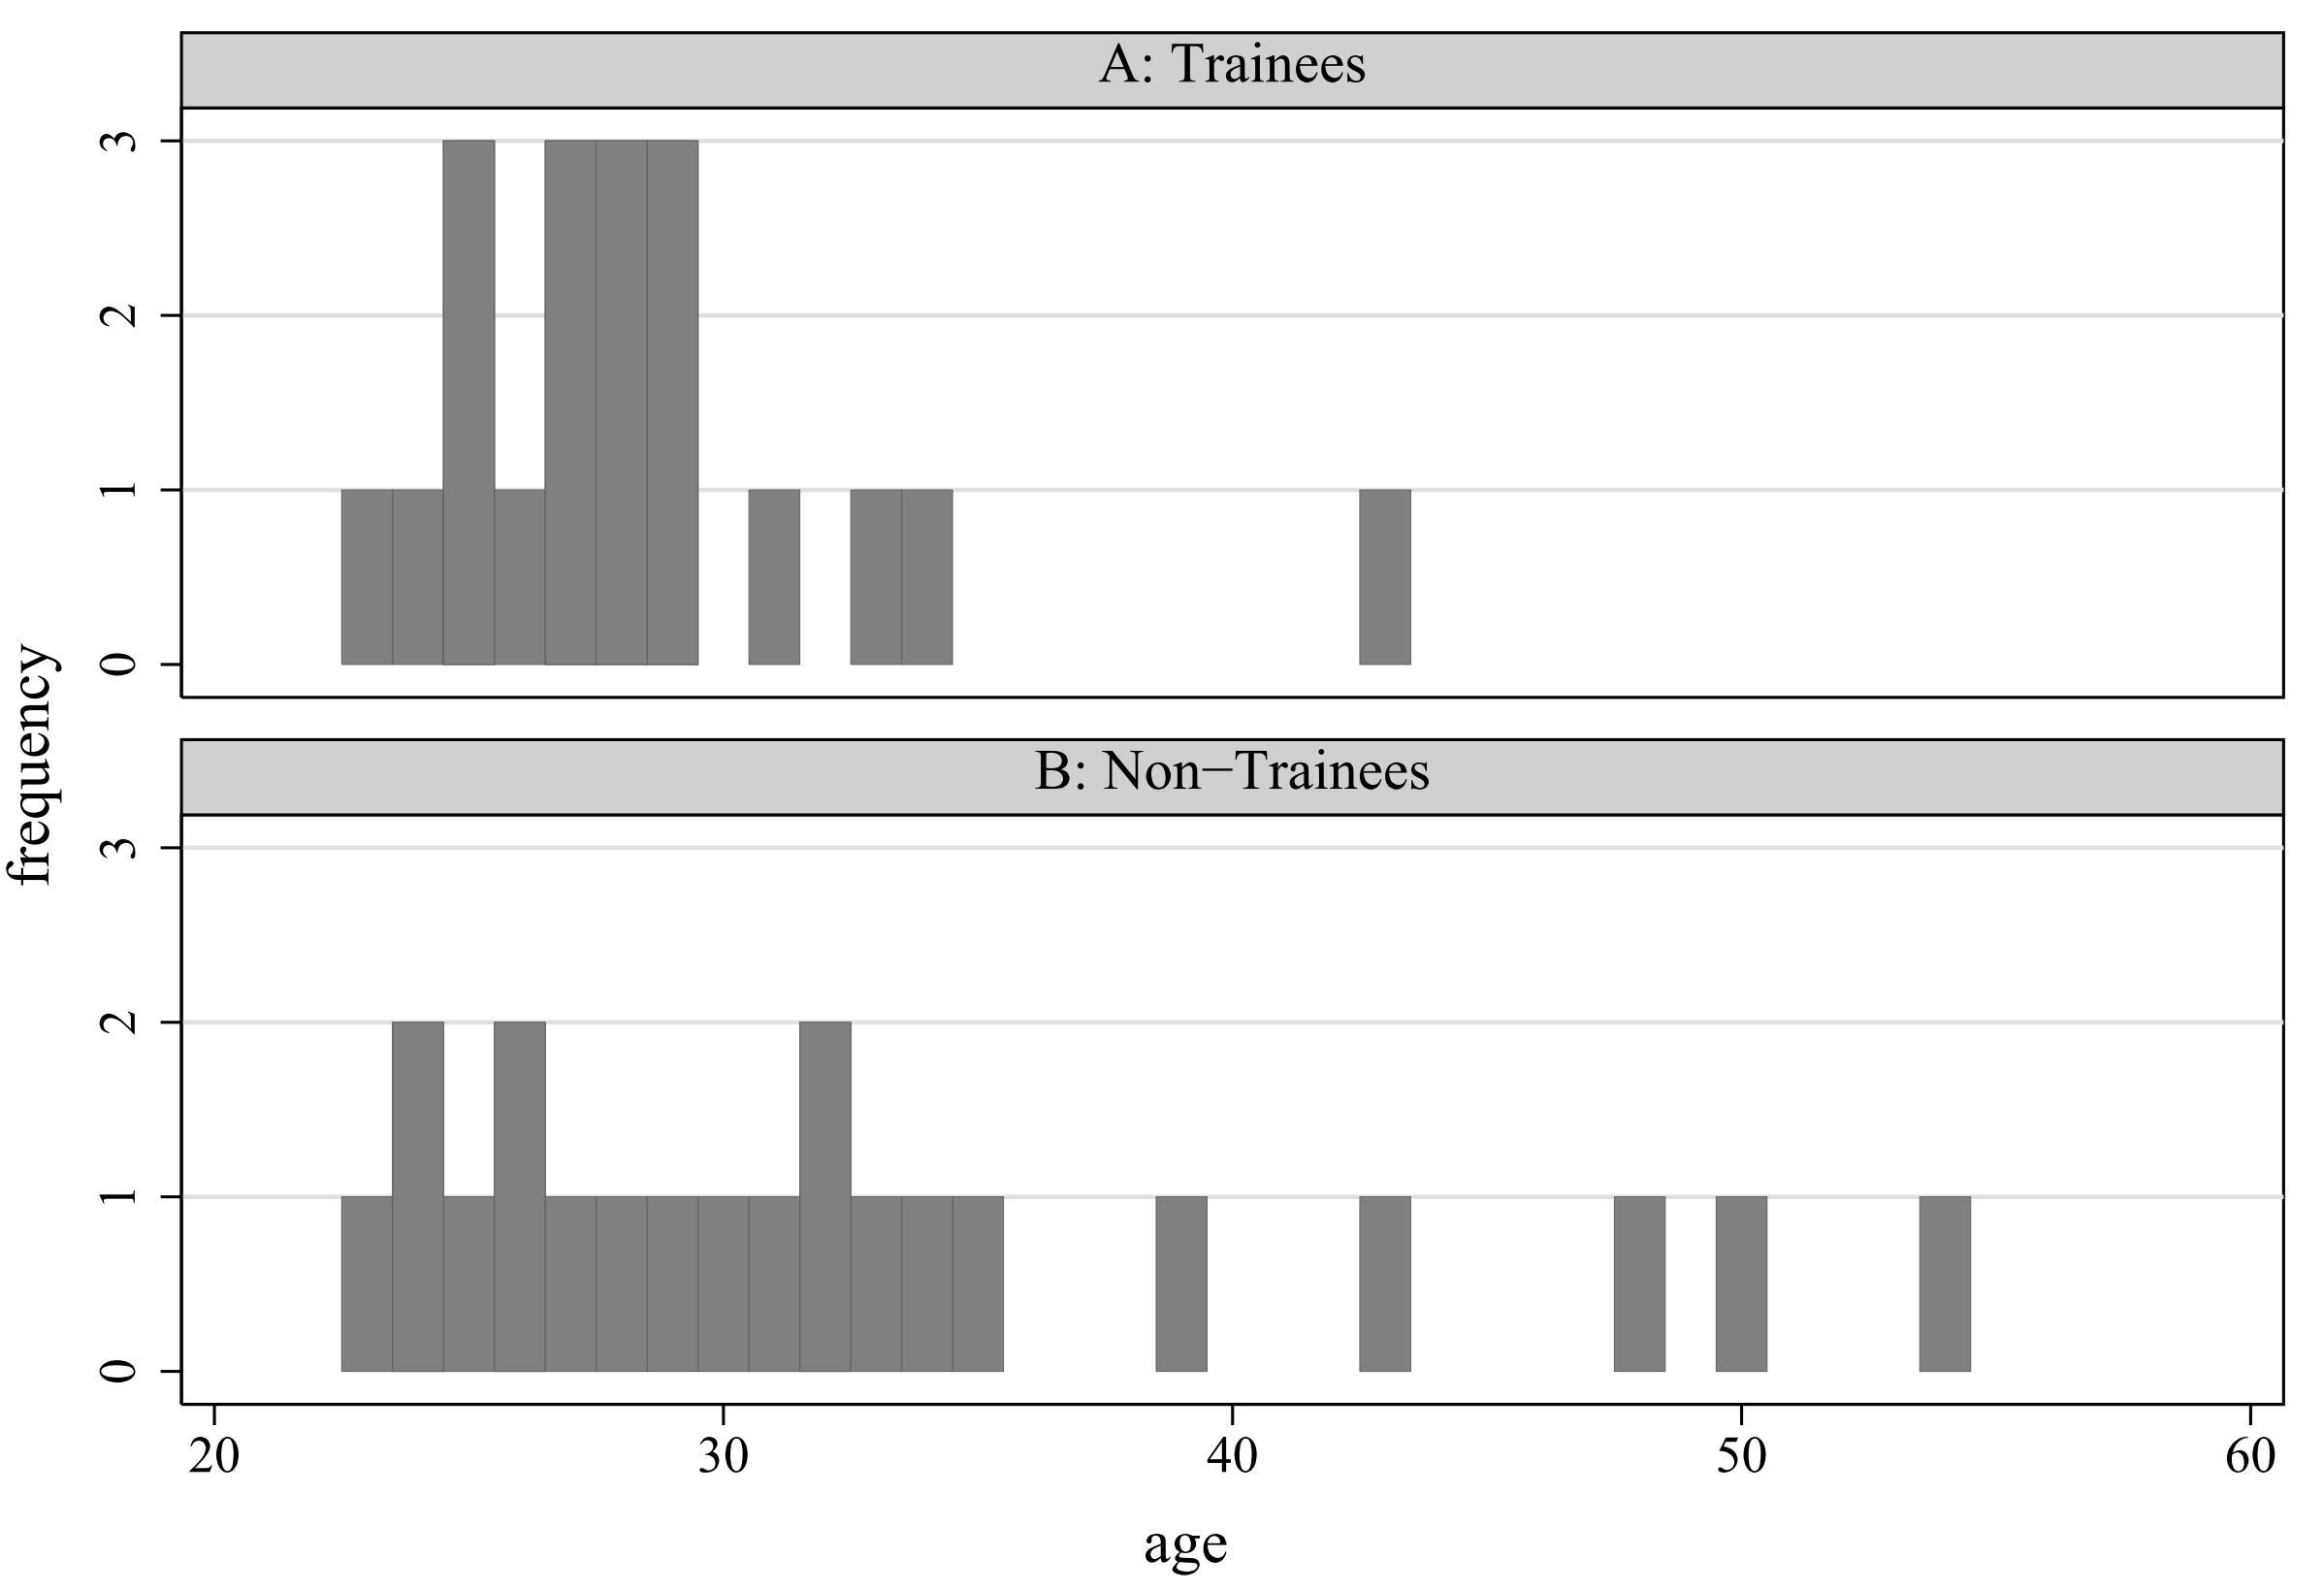
\includegraphics[width=0.9\textwidth]{figure/age_dis_before.jpg}
		\end{figure}
	\end{center}	
\end{frame}


\begin{frame}{Age Distribution: After Matching}
	\begin{center}
		\begin{figure}[p]
			\centering
			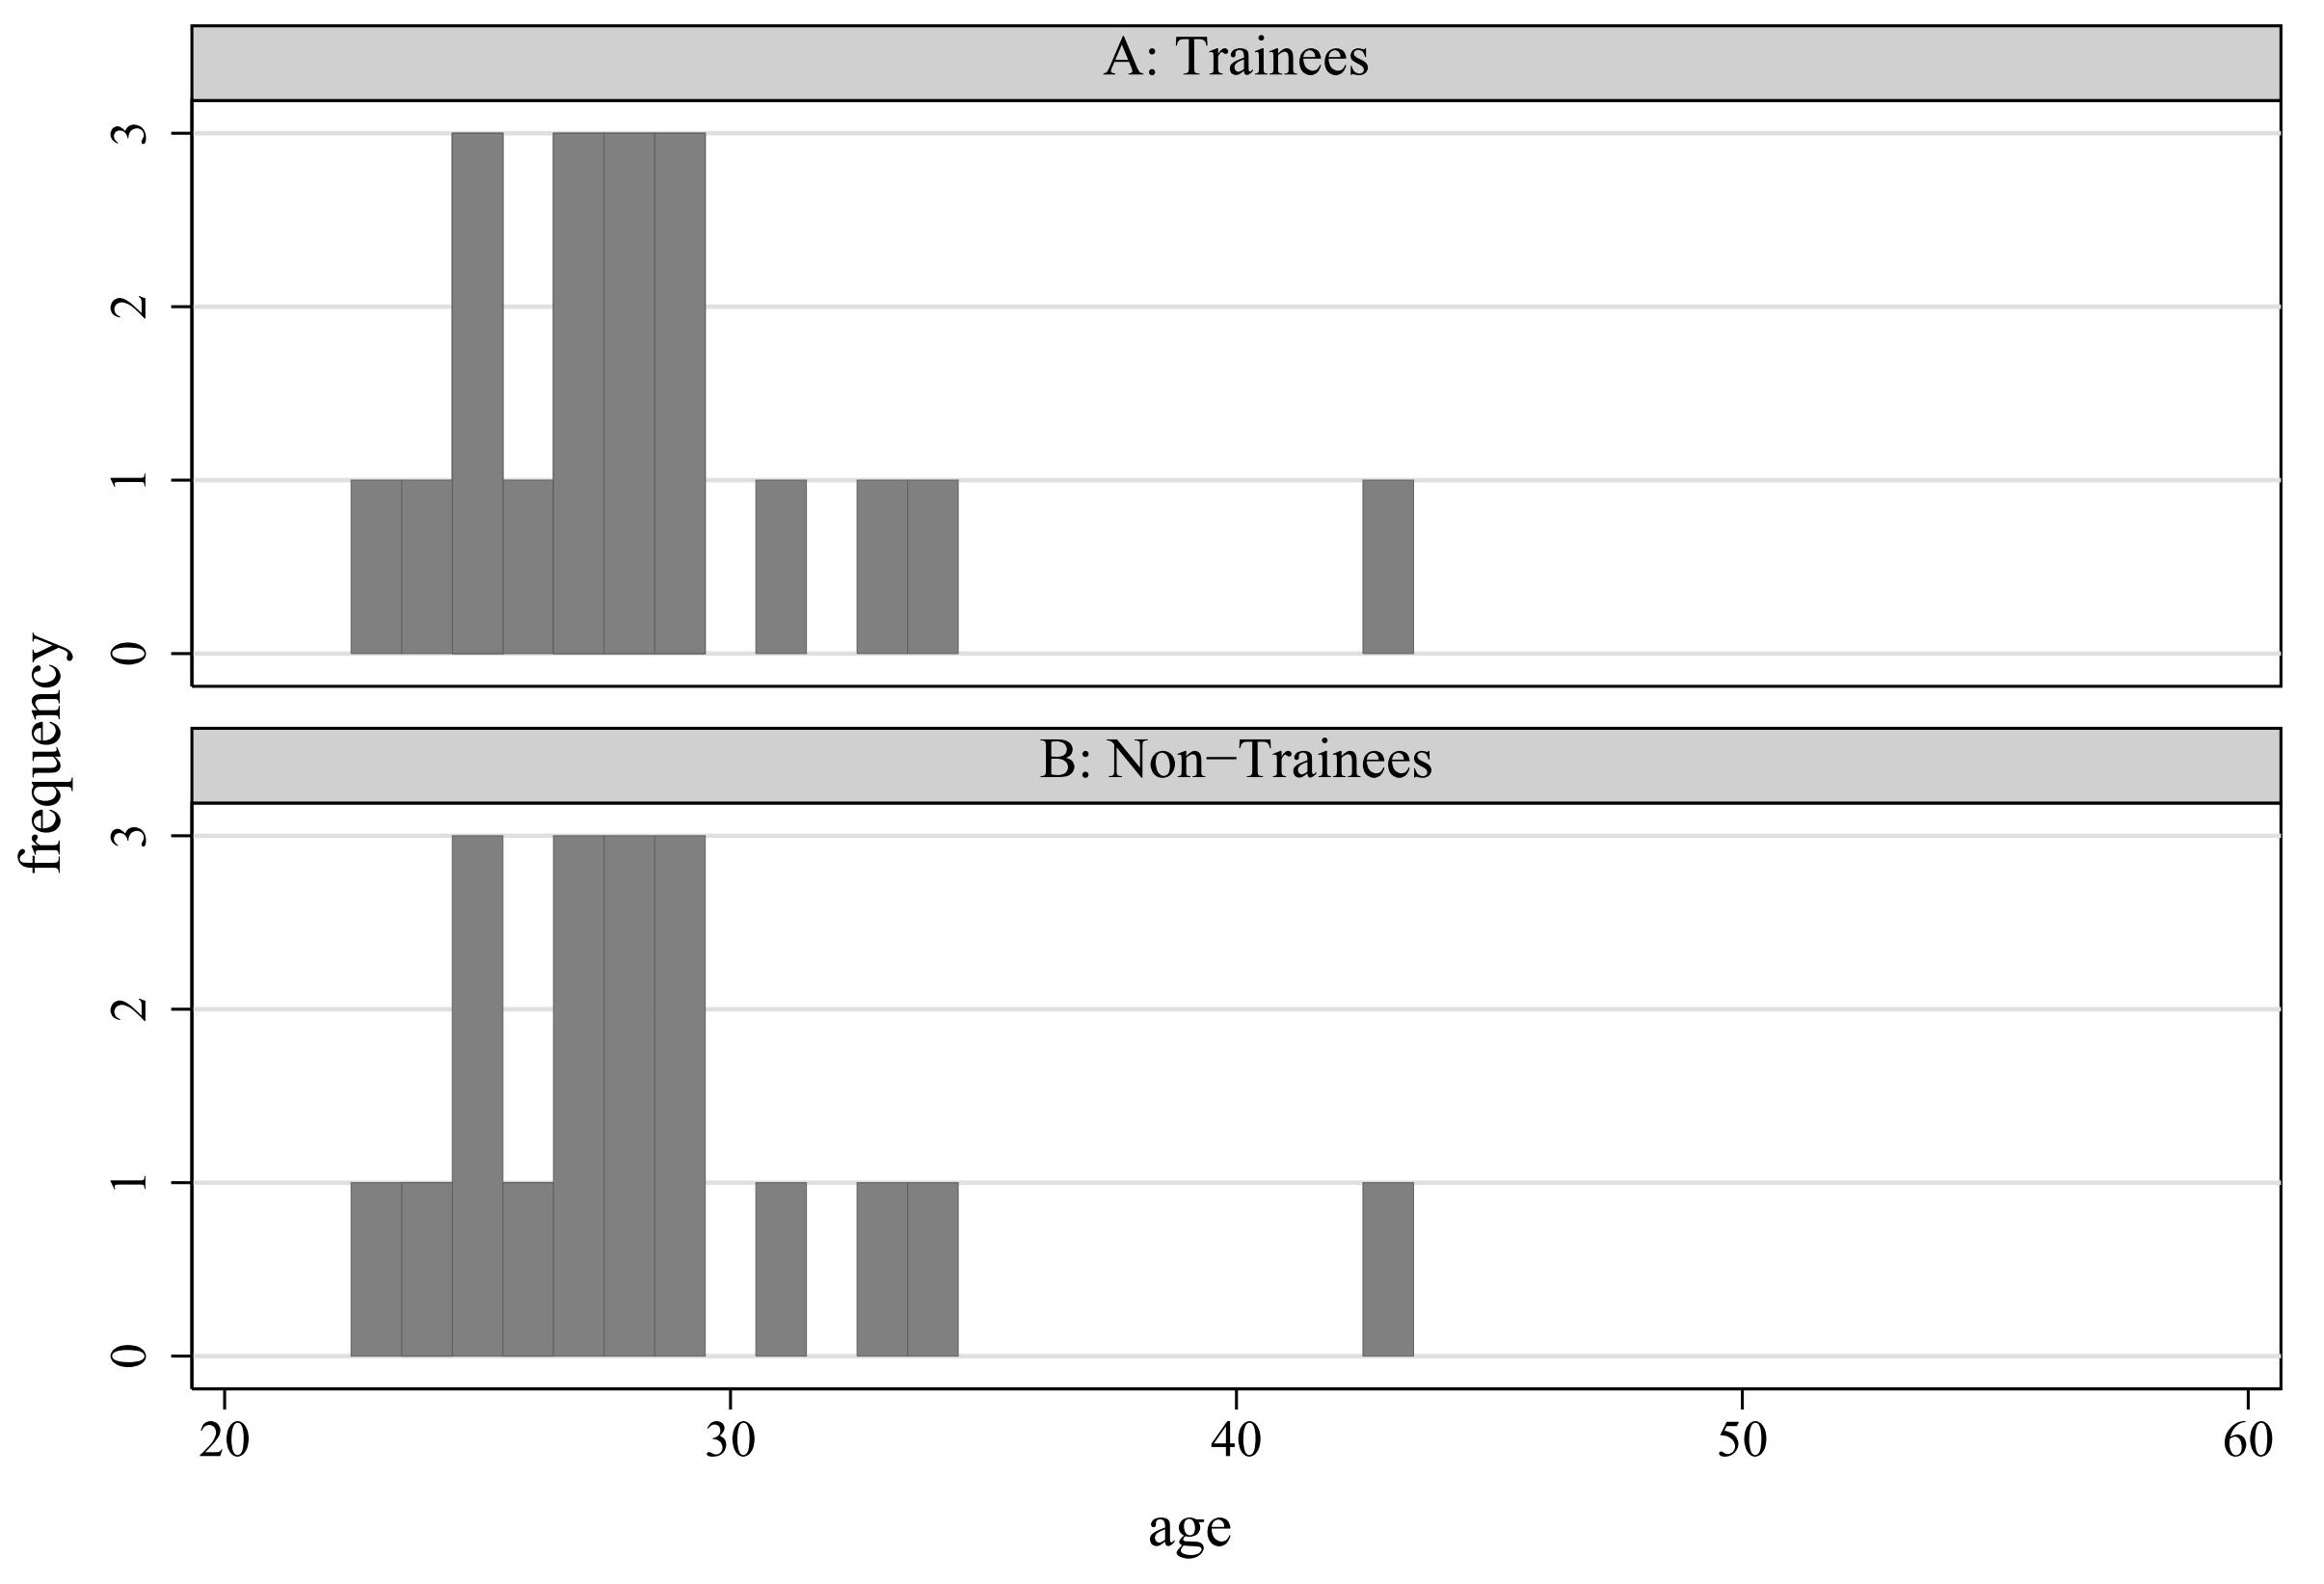
\includegraphics[width=0.9\textwidth]{figure/age_dis_after.jpg}
		\end{figure}
	\end{center}
\end{frame}


\begin{frame}{Treatment Effect Estimates}
	Difference in average earnings between trainees and non-trainees:
	\begin{itemize}
		\item Before matching:
		\begin{equation*}
		16426-20724=-4298
		\end{equation*}
		\item After matching:
		\begin{equation*}
		16426-13982=2444
		\end{equation*}
	\end{itemize}
\end{frame}


\title[]  
{Identification}


\author 
{}

\institute{}

\date
{}


\begin{frame}{}
	\titlepage
\end{frame}




\begin{frame}{Conditional Independence Assumption}
	\begin{block}{Conditional Independence Assumption (CIA)}
		\begin{equation*}
			(\mathrm{Y}^{1}_{i},\mathrm{Y}^{0}_{i})\indep D_{i}|X_{i}
		\end{equation*}
	\end{block}
	\begin{itemize}
		\item $(\mathrm{Y}^{1}_{i},\mathrm{Y}^{0}_{i})$ are potential outcomes and $D_{i}$ is the treatment indicator
		\vspace{0.2cm} 
		\item $X_{i}$ are observable characteristics (covariates) with value of $k$
		\vspace{0.2cm} 
		\item CIA asserts that conditional on observable characteristics $X_{i}$, potential outcomes are independent of treatment assignment
		\vspace{0.2cm}
		\begin{itemize}
			\item This assumption is also called \textbf{selection on observables}
		\end{itemize}
		\vspace{0.2cm}
		\item Intuition: After controlling for $X_{i}$, treatment assignment becomes ``as good as random"
	\end{itemize}
\end{frame}




\begin{frame}{Conditional Independence Assumption}{Example}
	\begin{itemize}
		
		\item Suppose \textbf{age} is the only confounding factor and we can control for it
		\vspace{0.2cm}
		\begin{itemize}
			\item Under CIA, for individuals of the same age, their decision to receive training is unrelated to their potential earnings
			\vspace{0.2cm}
		\end{itemize}
		\item That is, once controlling age, treatment and control group should be comparable (apple-to-apple comparison)
		\vspace{0.2cm}
		\begin{itemize}
			\item $\textcolor{red}{\mathrm{E}[\mathrm{Y}^{\textbf{0}}_{i}|X_{i}=40, D_i=1]}=\mathrm{E}[\mathrm{Y}^{\textbf{0}}_{i}|X_{i}=40, D_i=0]$
			\vspace{0.2cm}
					\begin{itemize}
			\item Estimate the \textbf{counterfactual} of what trainees would have earned without training using observed earnings of non-trainees
						\vspace{0.2cm}
			\end{itemize}
			\item $\textcolor{red}{\mathrm{E}[\mathrm{Y}^{\textbf{1}}_{i}|X_{i}=40, D_i=0]}=\mathrm{E}[\mathrm{Y}^{\textbf{1}}_{i}|X_{i}=40, D_i=1]$
			\vspace{0.2cm}
			\begin{itemize}
				\item Estimate the \textbf{counterfactual} of what non-trainees would have earned with training using observed earnings of trainees
			\end{itemize}
		\end{itemize}
		
	\end{itemize}
\end{frame}



\begin{frame}{Conditional Independence Assumption (CIA)}{Violation Example}
	\begin{itemize}
		\item If \textbf{motivation} affects both training enrollment and wage potential, but is \textbf{unobserved}, CIA fails
		\vspace{0.2cm}
		\begin{itemize}
			\item Highly motivated individuals are more likely to enroll in training ($D_i=1$)
			\vspace{0.2cm}
			\item These same individuals would earn more regardless of training
			\vspace{0.2cm}
			\item Therefore: $\mathrm{E}[\mathrm{Y}^{0}_{i}|X_{i}=40, D_i=1] > \mathrm{E}[\mathrm{Y}^{0}_{i}|X_{i}=40, D_i=0]$
		\end{itemize}
		\vspace{0.3cm}
		\item Consequences of CIA violation:
					\vspace{0.2cm}
		\begin{itemize}
			\item The treatment effect estimate will be \textbf{biased upward}
			\vspace{0.2cm}
			\item We would attribute higher earnings to the training effect, when part of the difference is actually due to motivation
			\vspace{0.2cm}
			\item In this case, our causal estimate still has \textbf{selection bias}
		\end{itemize}
	\end{itemize}
\end{frame}



\begin{frame}{Common Support Assumption}
	\begin{block}{Common Support Assumption}	
		\begin{equation*}
		0<\Pr(D_{i}=1|X_{i})<1  	
		\end{equation*}
	\end{block}
	\begin{itemize}
		\item For each value of covariates $X_{i}$, there is a positive probability of being both treated and untreated 
		\vspace{0.2cm}
		\item In other words, it is NOT possible to perfectly predict one's treatment status by using specific value of $X_{i}$
		\vspace{0.2cm}
		\begin{itemize}	
			\item For example, this excludes:
			\vspace{0.2cm}
					\begin{itemize}	
			\item All individuals with age 40 are in treatment group: $Pr(D_{i}=1|X_{i}=40)=1$
				\vspace{0.2cm}
			\item All individuals with age 40 are in control group: $Pr(D_{i}=1|X_{i}=40)=0$
				\end{itemize}
		\end{itemize}
				\vspace{0.2cm}
		\item It ensures sufficient overlap in characteristics of treated and untreated units to find adequate matched sample	
		
	\end{itemize}
\end{frame}




% -------------------------------------------------------
% Identification Results: Road Map
% -------------------------------------------------------

\begin{frame}{Identification Results for Matching}

	\begin{itemize}
		\item Under CIA and Common Support, matching can identify causal effects. We proceed in three steps:
		\vspace{0.3cm}
		\begin{itemize}
			\item[\textbf{Step 1}] Show that ODO at given $X_i$ equals \textbf{CATT} (selection bias = 0)
			\vspace{0.2cm}
			\item[\textbf{Step 2}] Under CIA, CATT = CATU = \textbf{CATE}
			\vspace{0.2cm}
			\item[\textbf{Step 3}] Apply LIE to average CATE over $X$ $\Rightarrow$ \textbf{ATT, ATU, ATE}
		\end{itemize}
	\end{itemize}
	
\end{frame}


% -------------------------------------------------------
% Step 1
% -------------------------------------------------------

\begin{frame}{Identification Results for Matching}{Step 1: ODO = CATT}
{\small
\begin{equation*}
\begin{aligned}
& 
\underbrace{\mathrm{E}[\mathrm{Y}_{i}|X_{i},D_{i}=1] - \mathrm{E}[\mathrm{Y}_{i}|X_{i},D_{i}=0]}_{\text{ODO at given } X_{i}}  \\
&=\mathrm{E}[\mathrm{Y}^{1}_{i}|X_{i},D_{i}=1] - \mathrm{E}[\mathrm{Y}^{0}_{i}|X_{i},D_{i}=0] \\
&= \mathrm{E}[\mathrm{Y}^{1}_{i}|X_{i},D_i=1]
-{\color{red} \mathrm{E}[\mathrm{Y}^{0}_{i}|X_{i},D_i=1]} \\
&\quad + {\color{red} \mathrm{E}[\mathrm{Y}^{0}_{i}|X_{i},D_i=1]}
-\mathrm{E}[\mathrm{Y}^{0}_{i}|X_{i},D_i=0] \\
&= \underbrace{\mathrm{E}[\mathrm{Y}^{1}_{i}-\mathrm{Y}^{0}_{i}|X_{i},D_i=1]}_{\text{CATT}} 
+ \underbrace{\mathrm{E}[\mathrm{Y}^{0}_{i}|X_{i},D_i=1]-\mathrm{E}[\mathrm{Y}^{0}_{i}|X_{i},D_i=0]}_{\scriptstyle\text{Selection Bias} = 0 \text{ by CIA}}  \\
&= \underbrace{\mathrm{E}[\mathrm{Y}^{1}_{i}-\mathrm{Y}^{0}_{i}|X_{i},D_i=1]}_{\text{CATT}}
\end{aligned}
\end{equation*}
}
\end{frame}


% -------------------------------------------------------
% Step 2  [FIX #1: removed nested $ in \text{}]
% -------------------------------------------------------

\begin{frame}{Identification Results for Matching}{Step 2: CATT = CATU = CATE}

	\begin{equation*}
		\begin{aligned}
		& 
			\underbrace{\mathrm{E}[\mathrm{Y}_{i}|X_{i},D_{i}=1] - \mathrm{E}[\mathrm{Y}_{i}|X_{i},D_{i}=0]}_{\text{ODO at given } X_{i}}  \\
			&= \underbrace{\mathrm{E}[\mathrm{Y}^{1}_{i}-\mathrm{Y}^{0}_{i}|X_{i},D_i=1]}_{\text{CATT}} \quad \text{(from Step 1)} \\[6pt]
			&= \underbrace{\mathrm{E}[\mathrm{Y}^{1}_{i}-\mathrm{Y}^{0}_{i}|X_{i},D_i=0]}_{\text{CATU}} \quad \text{(by CIA)} \\[6pt]
			&= \underbrace{\mathrm{E}[\mathrm{Y}^{1}_{i}-\mathrm{Y}^{0}_{i}|X_{i}]}_{\text{CATE}}
		\end{aligned}
	\end{equation*}	
	\begin{itemize}
		\item Under CIA, matching identifies the causal effect for \textbf{any given subgroup} $X_i = x$
	\end{itemize}
	
\end{frame}


% -------------------------------------------------------
% Review: LIE (merged into one slide)
% -------------------------------------------------------

\begin{frame}{Review: The Law of Iterated Expectations (LIE)}
	
	\begin{block}{The Law of Iterated Expectations (LIE)}
		\begin{equation*}
		\mathrm{E}[\mathrm{Y}_{i}] = \mathrm{E}[\mathrm{E}[\mathrm{Y}_{i} | \mathrm{X}_{i}]]
		\end{equation*}
	\end{block}
	
	\begin{itemize}
		\item Two equivalent ways to compute average earnings in Taiwan:
		\vspace{0.2cm}
		\item[1] Direct average: 40\% earn 1M, 40\% earn 2M, 20\% earn 3M
		\begin{equation*}
		\mathrm{E}[\mathrm{Y}_{i}] = 1 \times 0.4 + 2 \times 0.4 + 3 \times 0.2 = 1.8 \text{M}
		\end{equation*}
		\item[2] Average of subgroup averages: male avg = 2M, female avg = 1.6M, each 50\%
		\begin{equation*}
		\mathrm{E}[\mathrm{E}[\mathrm{Y}_{i}|\mathrm{X}_{i}]] = 2 \times 0.5 + 1.6 \times 0.5 = 1.8\text{M} = \mathrm{E}[\mathrm{Y}_{i}]
		\end{equation*}
		\vspace{0.1cm}
		\item Key insight: \textbf{average of subgroup averages = overall average}
	\end{itemize}
\end{frame}


% -------------------------------------------------------
% Step 3: ATT  [FIX #2: removed nested $ in \text{}]
% -------------------------------------------------------

\begin{frame}{Identification Results for Matching}{Step 3: From CATT to ATT}
	\begin{itemize}
		
		\item From Step 1, ODO at given $X_i$ identifies CATT:
		\begin{equation*}
			\underbrace{\mathrm{E}[\mathrm{Y}_{i}|X_{i},D_{i}=1] - \mathrm{E}[\mathrm{Y}_{i}|X_{i},D_{i}=0]}_{\text{ODO at given } X_{i}}  = \underbrace{\mathrm{E}[\mathrm{Y}^{1}_{i}-\mathrm{Y}^{0}_{i}|X_{i},D_i=1]}_{\text{CATT}}
		\end{equation*}	
		
		\item Applying LIE, average CATT over the \textbf{treatment group} distribution of $X$:
		
	\end{itemize}
	\begin{equation*}
		\mathrm{E}\Big[\underbrace{\mathrm{E}[\mathrm{Y}^{1}_{i}-\mathrm{Y}^{0}_{i}|X_{i},D_i=1]}_{\text{CATT}}\Big| D_i=1\Big] 
		=\underbrace{\mathrm{E}[\mathrm{Y}^{1}_{i}-\mathrm{Y}^{0}_{i}|D_i=1]}_{\text{ATT}}
	\end{equation*}	
	
\end{frame}


% -------------------------------------------------------
% ATT Numerical Example (kept as-is, two slides)
% -------------------------------------------------------

\begin{frame}{Identification Results for Matching: ATT}{A Numerical Example}
	\begin{center}
		\scalebox{0.75}{
			\begin{threeparttable}
				\centering\footnotesize
				\begin{tabular}{@{} ccrccrccr @{}}
					\multicolumn{3}{c}{Trainees} & \multicolumn{3}{c}{Non-Trainees} & \multicolumn{3}{c}{Matched Sample}\\
					\cmidrule(l){1-3}  \cmidrule(l){4-6} \cmidrule(l){7-9} 
					unit   & age   & earnings   & unit   & age   & earnings  & unit  & age   & earnings \\
					{\color{red}1} & {\color{red}28} & {\color{red}17700} &  1 & 43 & 20900 &  {\color{red}8} & {\color{red}28} & {\color{red}8800}   \\
					2 & 34 & 10200 &  2 & 50 & 31000 & 14 & 34 & 24200  \\ 
					3 & 29 & 14400 &  3 & 30 & 21000 & 17 & 29 & 6200   \\ 
					4 & 25 & 20800 &  4 & 27 & 9300  & 15 & 25 & 23300  \\  
					5 & 29 & 6100  &  5 & 54 & 41100 & 17 & 29 & 6200   \\
					6 & 23 & 28600 &  6 & 48 & 29800 & 20 & 23 & 9500   \\
					7 & 33 & 21900 &  7 & 39 & 42000 & 10 & 33 & 15500  \\
					8 & 27 & 28800 &  8 & 28 & 8800  &  4 & 27 & 9300   \\  
					9 & 31 & 20300 &  9 & 24 & 25500 & 12 & 31 & 26600  \\  
					10 & 26 & 28100 & 10 & 33 & 15500 & 11,13 & 26 & 8450   \\
					11 & 25 & 9400  & 11 & 26 & 400   & 15 & 25 & 23300  \\
					12 & 27 & 14300 & 12 & 31 & 26600 &  4 & 27 & 9300   \\
					13 & 29 & 12500 & 13 & 26 & 16500 & 17 & 29 & 6200   \\
					14 & 24 & 19700 & 14 & 34 & 24200 & 9,16 & 24 & 17700  \\
					15 & 25 & 10100 & 15 & 25 & 23300 & 15 & 25 & 23300  \\
					16 & 43 & 10700 & 16 & 24 & 9700  &  1 & 43 & 20900  \\ 
					{\color{red}17} & {\color{red}28} & {\color{red}11500} & 17 & 29 & 6200  & {\color{red}8} & {\color{red}28} & {\color{red}8800}   \\ 
					18 & 27 & 10700 & 18 & 35 & 30200 &  4 & 27 & 9300   \\
					{\color{red}19} & {\color{red}28} & {\color{red}16300} & 19 & 32 & 17800 &  {\color{red}8} & {\color{red}28} & {\color{red}8800}  \\ 
					&    &       & 20 & 23 & 9500  &    &  &   \\
					&    &       & 21 & 32 & 25900 &    &  &   \\ 
					\cmidrule(l){1-3}  \cmidrule(l){4-6} \cmidrule(l){7-9} 
					Avg: & 28.5 & 16426 & Avg: & 33 & 20724 & Avg: & 28.5 & 13982 \\
				\end{tabular}
		\end{threeparttable}}
	\end{center}
\end{frame}


\begin{frame}{Identification Results for Matching: ATT}{A Numerical Example}
	\begin{center}
		\scalebox{0.75}{
			\begin{threeparttable}
				\centering\footnotesize
				\begin{tabular}{@{} ccrccrccr @{}}
					\multicolumn{3}{c}{Trainees} & \multicolumn{3}{c}{Non-Trainees} & \multicolumn{3}{c}{Matched Sample}\\
					\cmidrule(l){1-3}  \cmidrule(l){4-6} \cmidrule(l){7-9} 
					unit   & age   & earnings   & unit   & age   & earnings  & unit  & age   & earnings \\
					1 & 28 & 17700 &  1 & 43 & 20900 &  8 & 28 & 8800   \\
					{\color{red}2} & {\color{red}34} & {\color{red}10200} &  2 & 50 & 31000 & {\color{red}14} & {\color{red}34} & {\color{red}24200}  \\ 
					3 & 29 & 14400 &  3 & 30 & 21000 & 17 & 29 & 6200   \\ 
					4 & 25 & 20800 &  4 & 27 & 9300  & 15 & 25 & 23300  \\  
					5 & 29 & 6100  &  5 & 54 & 41100 & 17 & 29 & 6200   \\
					6 & 23 & 28600 &  6 & 48 & 29800 & 20 & 23 & 9500   \\
					7 & 33 & 21900 &  7 & 39 & 42000 & 10 & 33 & 15500  \\
					8 & 27 & 28800 &  8 & 28 & 8800  &  4 & 27 & 9300   \\  
					9 & 31 & 20300 &  9 & 24 & 25500 & 12 & 31 & 26600  \\  
					10 & 26 & 28100 & 10 & 33 & 15500 & 11,13 & 26 & 8450   \\
					11 & 25 & 9400  & 11 & 26 & 400   & 15 & 25 & 23300  \\
					12 & 27 & 14300 & 12 & 31 & 26600 &  4 & 27 & 9300   \\
					13 & 29 & 12500 & 13 & 26 & 16500 & 17 & 29 & 6200   \\
					14 & 24 & 19700 & 14 & 34 & 24200 & 9,16 & 24 & 17700  \\
					15 & 25 & 10100 & 15 & 25 & 23300 & 15 & 25 & 23300  \\
					16 & 43 & 10700 & 16 & 24 & 9700  &  1 & 43 & 20900  \\ 
					17 & 28 & 11500 & 17 & 29 & 6200  &  8 & 28 & 8800   \\ 
					18 & 27 & 10700 & 18 & 35 & 30200 &  4 & 27 & 9300   \\
					19 & 28 & 16300 & 19 & 32 & 17800 &  8 & 28 & 8800  \\ 
					&    &       & 20 & 23 & 9500  &    &  &   \\
					&    &       & 21 & 32 & 25900 &    &  &   \\ 
					\cmidrule(l){1-3}  \cmidrule(l){4-6} \cmidrule(l){7-9} 
					Avg: & 28.5 & 16426 & Avg: & 33 & 20724 & Avg: & 28.5 & 13982 \\
				\end{tabular}
		\end{threeparttable}}
	\end{center}
\end{frame}


\begin{frame}{Identification Results for Matching: ATT}{A Numerical Example (1/2)}
	\begin{itemize}
		\item CATT for age = 28 and age = 34:
		\vspace{0.2cm}
		\begin{equation*}
			\begin{aligned}
				& \mathrm{E}[\mathrm{Y}^{1}_{i}-\mathrm{Y}^{0}_{i}|X_{i}=28, D_{i}=1] \\
				&= \dfrac{(17700-8800)+(11500-8800)+(16300-8800)}{3} \\
				&= 6366.67 \\[10pt]
				& \mathrm{E}[\mathrm{Y}^{1}_{i}-\mathrm{Y}^{0}_{i}|X_{i}=34, D_{i}=1] \\
				&= \dfrac{10200-24200}{1} \\
				&= -14{,}000 \quad \cdots
			\end{aligned} 
		\end{equation*}	
	\end{itemize}
\end{frame}


\begin{frame}{Identification Results for Matching: ATT}{A Numerical Example (2/2)}
	\begin{itemize}
		\item ATT = weighted average of CATT across all ages \\
		(weights = share in treatment group):
		\vspace{0.2cm}
		\begin{equation*}
			\begin{aligned}
				\mathrm{ATT} 
				&= \mathrm{E}[\mathrm{Y}^{1}_{i}-\mathrm{Y}^{0}_{i}|X_{i}=28, D_{i}=1] \times \frac{3}{19} \\  
				&\quad + \mathrm{E}[\mathrm{Y}^{1}_{i}-\mathrm{Y}^{0}_{i}|X_{i}=34, D_{i}=1] \times \frac{1}{19} + \cdots \\[6pt]
				&= \underbrace{\mathrm{E}[\mathrm{Y}^{1}_{i}-\mathrm{Y}^{0}_{i}|D_{i}=1]}_{\text{ATT}}
			\end{aligned}
		\end{equation*}	
	\end{itemize}
\end{frame}


% -------------------------------------------------------
% ATU and ATE (concise)
% -------------------------------------------------------

\begin{frame}{Identification Results for Matching}{Step 3: ATU and ATE}
	\begin{itemize}
		
		\item \textbf{ATU}: average CATU over the \textbf{control group} distribution of $X$:
		\begin{equation*}
			\mathrm{E}\Big[\underbrace{\mathrm{E}[\mathrm{Y}^{1}_{i}-\mathrm{Y}^{0}_{i}|X_{i},D_i=0]}_{\text{CATU}}\Big| D_i=0\Big] 
			=\underbrace{\mathrm{E}[\mathrm{Y}^{1}_{i}-\mathrm{Y}^{0}_{i}|D_i=0]}_{\text{ATU}}
		\end{equation*}
		
		\vspace{0.2cm}
		\item \textbf{ATE}: average CATE over the \textbf{full population} distribution of $X$:
		\begin{equation*}
			\mathrm{E}\Big[\underbrace{\mathrm{E}[\mathrm{Y}^{1}_{i}-\mathrm{Y}^{0}_{i}|X_{i}]}_{\text{CATE}}\Big] 
			=\underbrace{\mathrm{E}[\mathrm{Y}^{1}_{i}-\mathrm{Y}^{0}_{i}]}_{\text{ATE}}
		\end{equation*}
		
		\vspace{0.2cm}
		\item \textbf{Summary}: Under CIA, matching can identify ATT, ATU, and ATE by averaging $X$-specific effects over the appropriate population
		
	\end{itemize}
\end{frame}




\title[]  
{Estimation}


\author 
{}

\institute{}

\date
{}


\begin{frame}{}
\titlepage
\end{frame}


\begin{frame}{Matching Estimator}
\begin{itemize}
	
\item Suppose our sample is $N$ individuals
\vspace{0.3cm}
\item Treatment is job training and outcome is earning
\vspace{0.3cm}
\begin{itemize}
	\item $N_1$ individuals choose to join job training: treatment group
	\vspace{0.3cm}
	\item $N_0$ individuals choose not join it ($N_0=N-N_1$): control group
\end{itemize}

\end{itemize}
\end{frame}



\begin{frame}{Matching Estimator}{Estimation for ATT}
	\begin{itemize}

		\item Suppose we want to estimate ATT
		\vspace{0.3cm}
			\begin{itemize}
			\item Average treatment effect for treatment group
					\vspace{0.3cm}
		\end{itemize}
		\item In that case, a matching estimator of $\alpha_{\text{ATT}}$ can be constructed as:
		\begin{equation*}
		\hat{\alpha}_{\text{ATT}}=\dfrac{1}{N_1}\sum_{D_i=1}(Y_i-Y_{j(i)})
		\end{equation*}
		
			\begin{itemize}
			\item We want to match \textbf{treated} individual $i$'s outcome $Y_i$
		\vspace{0.3cm}
					\begin{itemize}
		\item We impute $Y^{0}_{i}$ using untreated units $Y_{j(i)}$ in control group
				\vspace{0.3cm}
		\item $Y_{j(i)}$: the outcome of an untreated observation $j$ such that $X_{j(i)}$ is the \textbf{same} or \textbf{closest} value to $X_i$ among the untreated observations. 
					\end{itemize}
			\end{itemize}
		
	\end{itemize}
\end{frame}


\begin{frame}{Matching Estimator}{Estimation for ATT}
\begin{itemize}
	
\item We can also use the average:
	\begin{equation*}
	\hat{\alpha}_{\text{}ATT}=\dfrac{1}{N_1}\sum_{D_i=1}\left\lbrace Y_i-\left(\dfrac{1}{M}\sum^M_{m=1}Y_{jm(i)}\right)\right\rbrace
	\end{equation*}
\item Works well when we can find good matches for each treated unit, so $M$ is usually small (typically, $M=1$ or $M=2$)
\vspace{0.3cm}
		\item Perfect matches are often not available 

\end{itemize}
\end{frame}




\begin{frame}{Matching Estimator}{Estimation for ATU}
	\begin{itemize}
		
		\item Suppose we want to estimate ATU 
				\vspace{0.3cm}
			\begin{itemize}
		\item Average treatment effect for control group
		
				\end{itemize}
		\vspace{0.3cm}
		\item In that case, a matching estimator of $\alpha_{\text{ATU}}$ can be constructed as:
		\begin{equation*}
		\hat{\alpha}_{\text{ATU}}=\dfrac{1}{N_0}\sum_{D_i=0}(Y_{j(i)}-Y_i)
		\end{equation*}
		
		\begin{itemize}
			
			\item We want to match \textbf{untreated} individual $i$'s outcome $Y_i$
					\vspace{0.3cm}
							\begin{itemize}
			\item We impute $Y^{1}_{i}$ using treated units $Y_{j(i)}$ in treatment group	
								\vspace{0.3cm}	
			\item $Y_{j(i)}$: the outcome of an treated observation $j$ such that $X_{j(i)}$ is the \textbf{same} or \textbf{closest} value to $X_i$ among the treated observations. 
					\end{itemize}
		\end{itemize}
		
	\end{itemize}
\end{frame}


\begin{frame}{Matching}{Estimation for ATE}
\begin{itemize}
\item We can also use matching to estimate ATE 
\vspace{0.2cm}
	\begin{itemize}
	\item Average treatment effect for both treatment and control groups
	\vspace{0.2cm}
\end{itemize}

\item In that case, we match in both directions:
\vspace{0.2cm}
\begin{itemize}
\item[1.] If observation $i$ is treated, we impute $Y^{0}_{i}$ using untreated units $Y_{j(i)}$ in control group
\vspace{0.2cm}
\item[2.] If observation $i$ is untreated, we impute $Y^{1}_{i}$ using treated units $Y_{j(i)}$ in treatment group
\end{itemize}
\vspace{0.2cm}
\item The matching estimator for ATE is:
	\begin{equation*}
	\hat{\alpha}_{\text{ATE}}=\dfrac{1}{N}\left\lbrace \sum_{D_i=1}(Y_i-Y_{j(i)})+\sum_{D_i=0}(Y_{j(i)}-Y_i)\right\rbrace
	\end{equation*}
\end{itemize}
\end{frame}


\begin{frame}{Exact Matching}{}
	\begin{itemize}
		
		\item Match each treated unit to a control unit that has exactly the same covariate
		values
		\vspace{0.2cm}	
		\item This is called \textbf{exact matching} and can be thought of as the gold standard for
		matching
	
	\end{itemize}
\end{frame}


\begin{frame}{Exact Matching}{A Numerical Example}
	\begin{center}
		\begin{figure}[p]
			\centering
			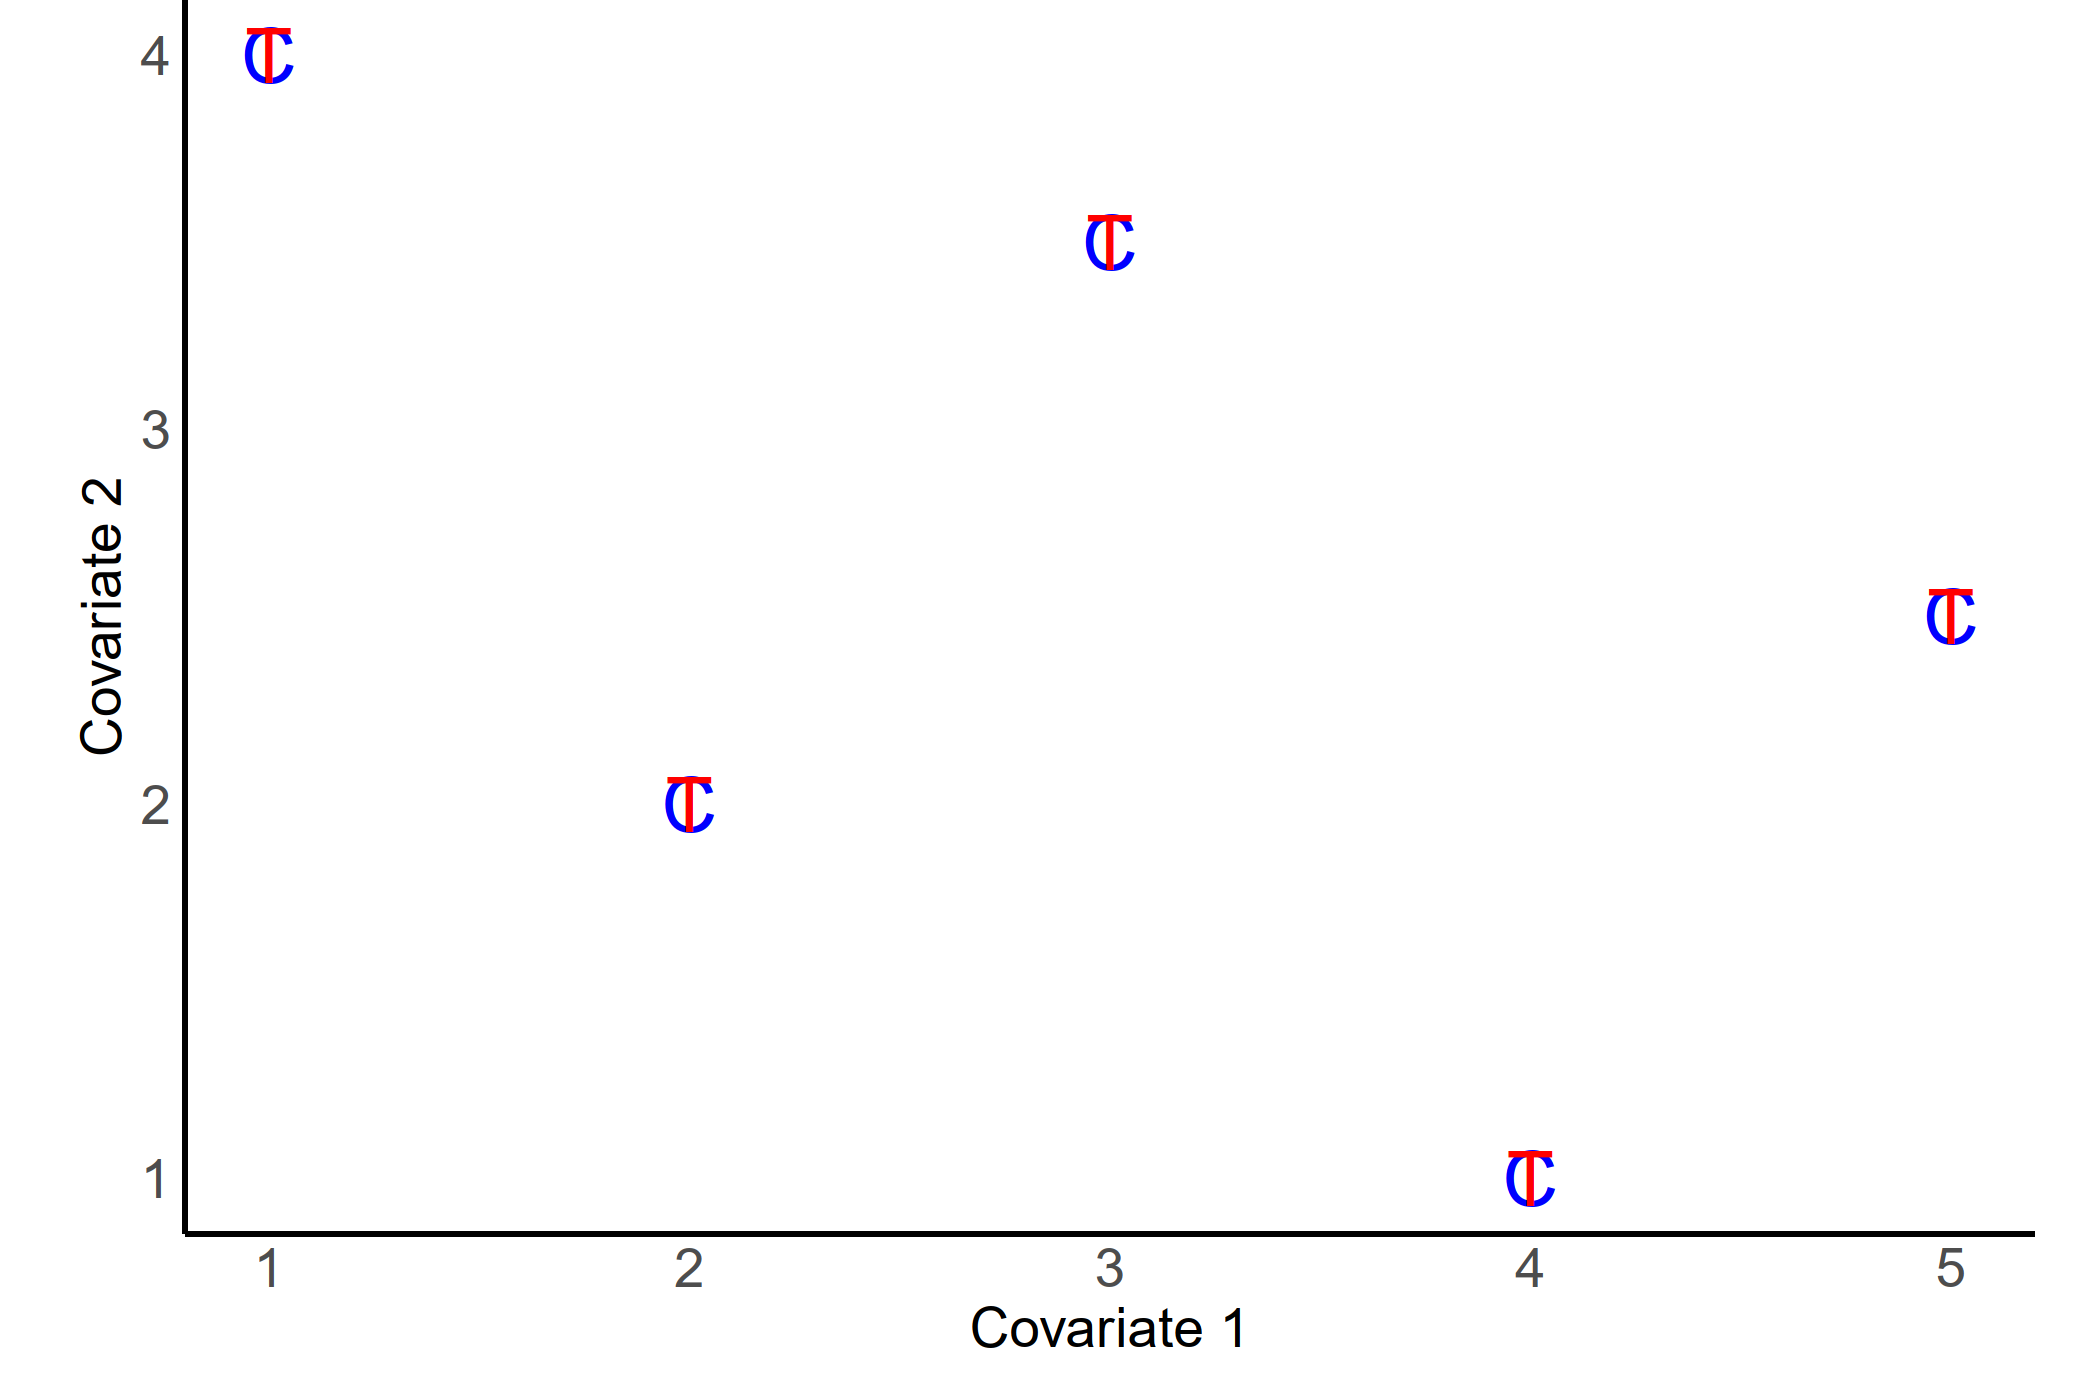
\includegraphics[width=0.8\textwidth]{figure/em_f1.png}
		\end{figure}
		\begin{minipage}{0.9\linewidth}
			\fontsize{8}{8pt}\selectfont
			\emph{Source:} Ben Elsner's slides
		\end{minipage}
	\end{center}
\end{frame}


\begin{frame}{Exact Matching and the ``Curse of Dimensionality"}
	\begin{itemize}
		\item Matching becomes unfeasible with many covariates
		\vspace{0.2cm}
		\item This is also true even if we divided each of covariates into coarse categories (subclassification)
	\end{itemize}
\end{frame}


\begin{frame}{Exact Matching and the ``Curse of Dimensionality"}
	\begin{itemize}
		\item Assume we have $k$ covariates and divided each of them into 3 coarse categories 
		\vspace{0.2cm}
		\begin{itemize}
			\item age could be ``young", ``middle age" or ``old"
			\vspace{0.2cm}
			\item income could be ``low", ``medium" or ``high"
		\end{itemize}
		\vspace{0.2cm}
		\item The number of subclassification cells is $3^k$. 
		\begin{itemize}
			\vspace{0.2cm}
			\item For $k=10$, we obtain $3^{10}=59049$
		\end{itemize}
		\vspace{0.2cm}
		\item Many cells may contain only treated or untreated observations
		\vspace{0.2cm}
		\begin{itemize}
			\item We may not be able to construct matched sample
			\vspace{0.2cm}
			\item Violate common support assumption
		\end{itemize}
	\end{itemize}
\end{frame}


\begin{frame}{Approximate Matching}{}
	\begin{itemize}
		
		\item In most cases, we just match similar units 
		\vspace{0.2cm}	
		\item This is called \textbf{approximate matching}
		\vspace{0.2cm}	
		\item There are three main methods for approximate matching:
				\vspace{0.2cm}	
		\begin{itemize}
			\item[1] \textbf{Distance Matching:} minimize distance in covariates $X$
			\vspace{0.2cm}
			\item[2] \textbf{Coarsened Exact Matching:}	match within coarsened subgroups
			\vspace{0.2cm}
			\item[3] \textbf{Propensity Score Matching:} match on likelihood of being treated
						
		\end{itemize}
	\end{itemize}
\end{frame}


\begin{frame}{Distance Matching}{Measure Closeness}
\begin{itemize}
	
\item We usually use more than one characteristics to construct a matched sample
\vspace{0.2cm}	
\item When the vector of matching covariates has more than one variables (h>1) 
	\begin{align*}
	X=\left(
	\begin{array}{c}
	X_1\\X_2\\\vdots\\X_H
	\end{array}\right)
	\end{align*}

\item We need to define a \textbf{distance metric} to measure ``closeness" to construct a matched sample

\end{itemize}
\end{frame}


\begin{frame}{Distance Matching}{Measure Closeness}
\begin{itemize}

\item The usual \textbf{Euclidean distance} is:
	\begin{equation*}
	\begin{aligned}
	||X_i-X_j||&=\sqrt{(X_i-X_j)'(X_i-X_j)} \\
	&=\sqrt{\sum^H_{h=1}(X_{hi}-X_{hj})^2}.
	\end{aligned}	
	\end{equation*}
\begin{itemize}
	
\item Sum up the differences between treatment group and control group over $h$ characteristics	
	\vspace{0.2cm}	
	\begin{itemize}
\item\textbf{Drawback:} The Euclidean distance is NOT invariant to changes in the scale of the $X$'s
\vspace{0.2cm}
\item For this reason, we often use alternative distances that are invariant to changes in scale
\end{itemize}

\end{itemize}
\end{itemize}
\end{frame}


\begin{frame}{Distance Matching}{Measure Closeness}
\begin{itemize}

\item A commonly used distance is the \textbf{normalized Euclidean distance}
	\begin{equation*}
	||X_i-X_j||=\sqrt{(X_i-X_j)'\widehat{V}^{-1}(X_i-X_j)} 
	\end{equation*}
where
	\begin{align*}
	\hat{V}=\left(
	\begin{array}{cccc}
	\hat{\sigma}^2_1& 0& ...& 0 \\
	0 & \hat{\sigma}^2_2 & ... & 0 \\
	\vdots & \vdots & \ddots & \vdots \\
	0 & 0 & ... & \hat{\sigma}^2_H
	\end{array}\right).
	\end{align*}
	\item $\hat{\sigma}^2_{h}$ is the variance of variable $h$	
\vspace{0.2cm}

\end{itemize}
\end{frame}


\begin{frame}{Distance Matching}{Measure Closeness}
	\begin{itemize}
		
		\item Notice that, the normalized Euclidean distance is equal to:
		\begin{equation*}
		||X_i-X_j||=\sqrt{\sum^H_{h=1}\dfrac{(X_{hi}-X_{hj})^2}{\hat{\sigma}^2_h}}.
		\end{equation*}
		\begin{itemize}
			\item[$\Rightarrow$] Changes in the scale of $X_{ki}$ affect also $\hat{\sigma}_k$, and the normalized Euclidean distance does not change
		\end{itemize}
		
	\end{itemize}
\end{frame}


\begin{frame}{Distance Matching}{Criteria for a Good Match}
	\begin{itemize}
		
		\item k-Nearest-neighbor Matching
		\vspace{0.2cm}	
		\begin{itemize}
			\item Match with the nearest neighbor or the k nearest neighbors in terms of normalized Euclidean distance 
			\vspace{0.2cm}
			\item Drop the unmatched units
						\vspace{0.2cm}
		\end{itemize}
	
	\item Radius Matching
		\vspace{0.2cm}	
	\begin{itemize}
		\item Match with all control units within a certain radius of the treated unit
	\end{itemize}
	
	\end{itemize}
\end{frame}


\begin{frame}{Distance Matching}{k-Nearest-neighbor Matching: k=1}
	\begin{center}
		\begin{figure}[p]
			\centering
			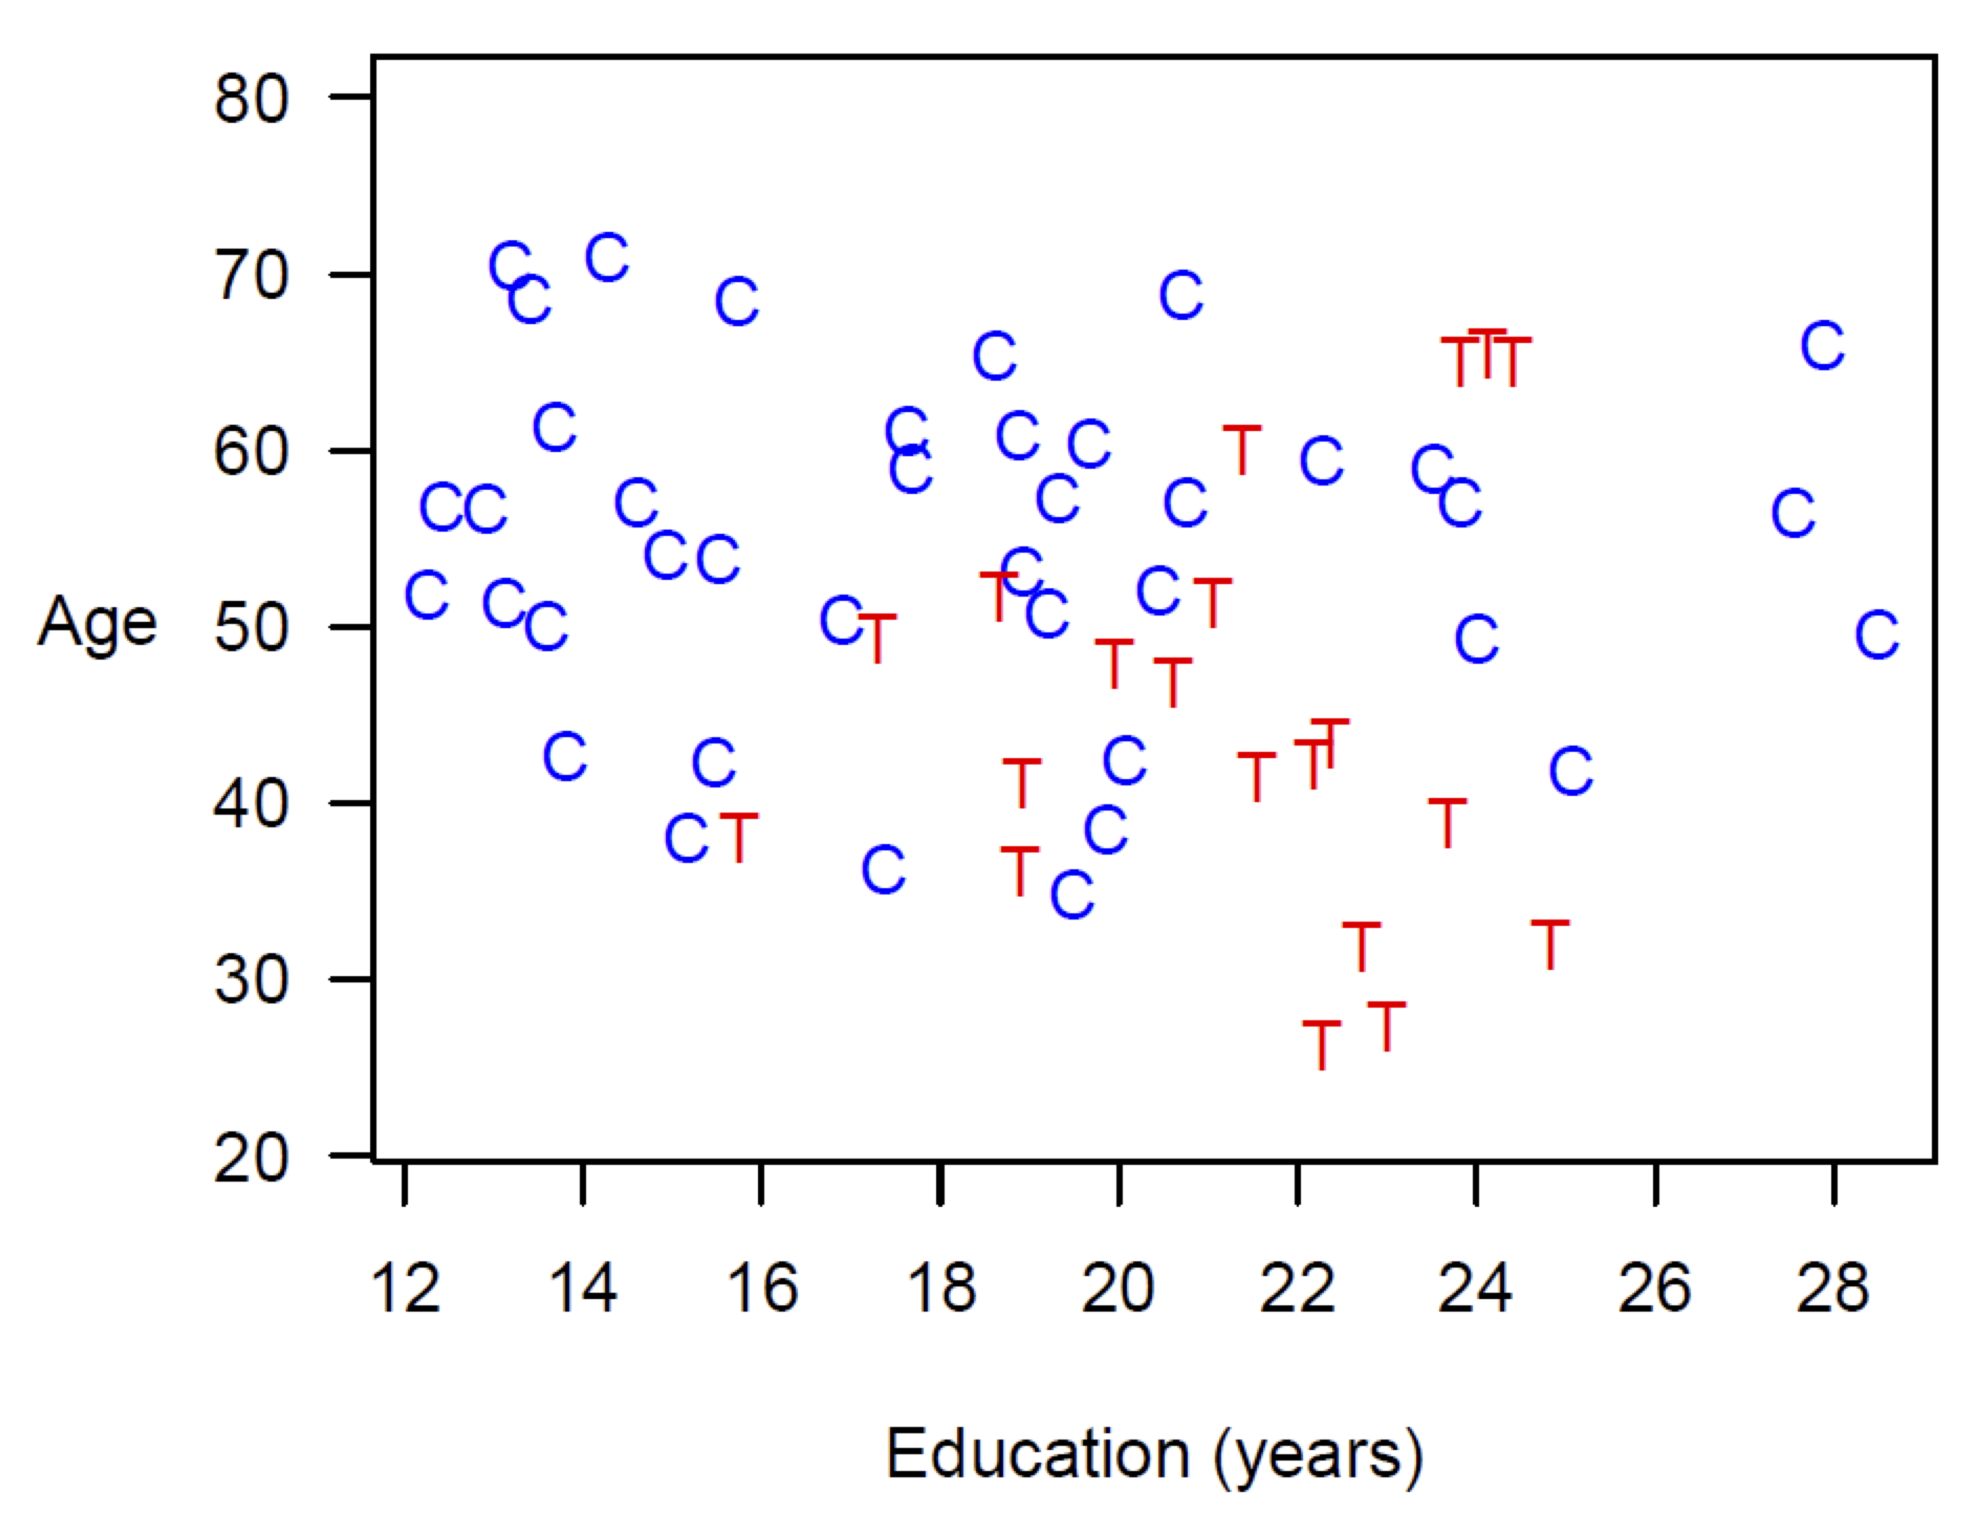
\includegraphics[width=0.7\textwidth]{figure/dm_f1.png}
		\end{figure}
		\begin{minipage}{0.9\linewidth}
			\fontsize{8}{8pt}\selectfont
			\emph{Source:} Ben Elsner's slides
		\end{minipage}
	\end{center}
\end{frame}


\begin{frame}{Distance Matching}{k-Nearest-neighbor Matching: k=1}
	\begin{center}
		\begin{figure}[p]
			\centering
			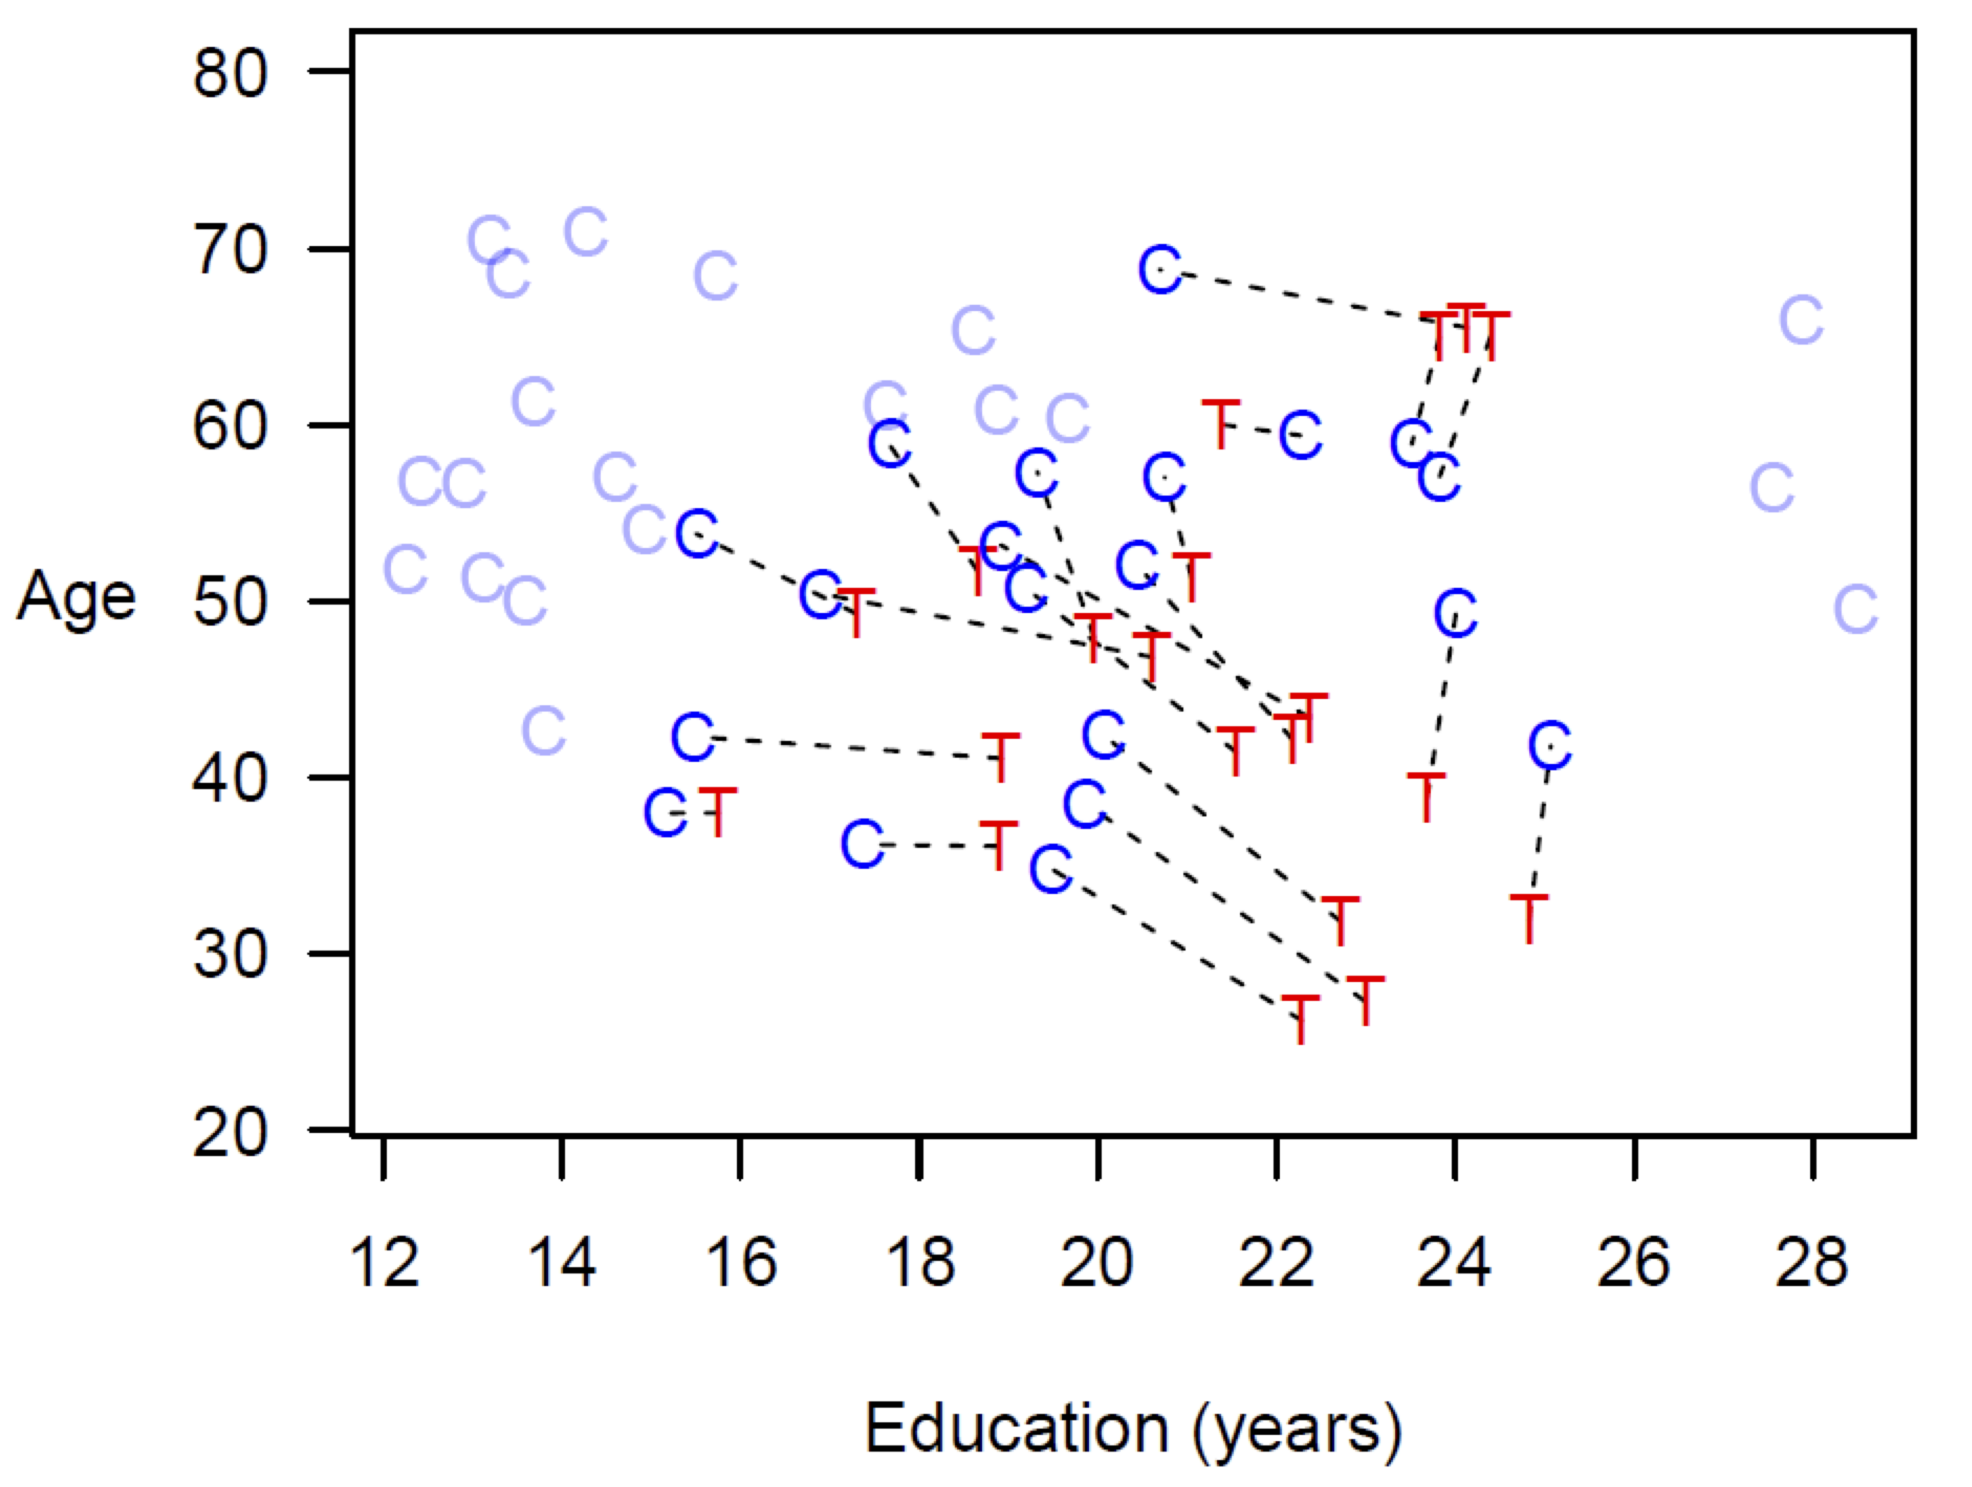
\includegraphics[width=0.7\textwidth]{figure/dm_f2.png}
		\end{figure}
		\begin{minipage}{0.9\linewidth}
			\fontsize{8}{8pt}\selectfont
			\emph{Source:} Ben Elsner's slides
		\end{minipage}
	\end{center}
\end{frame}


\begin{frame}{Distance Matching}{k-Nearest-neighbor Matching: k=1}
	\begin{center}
		\begin{figure}[p]
			\centering
			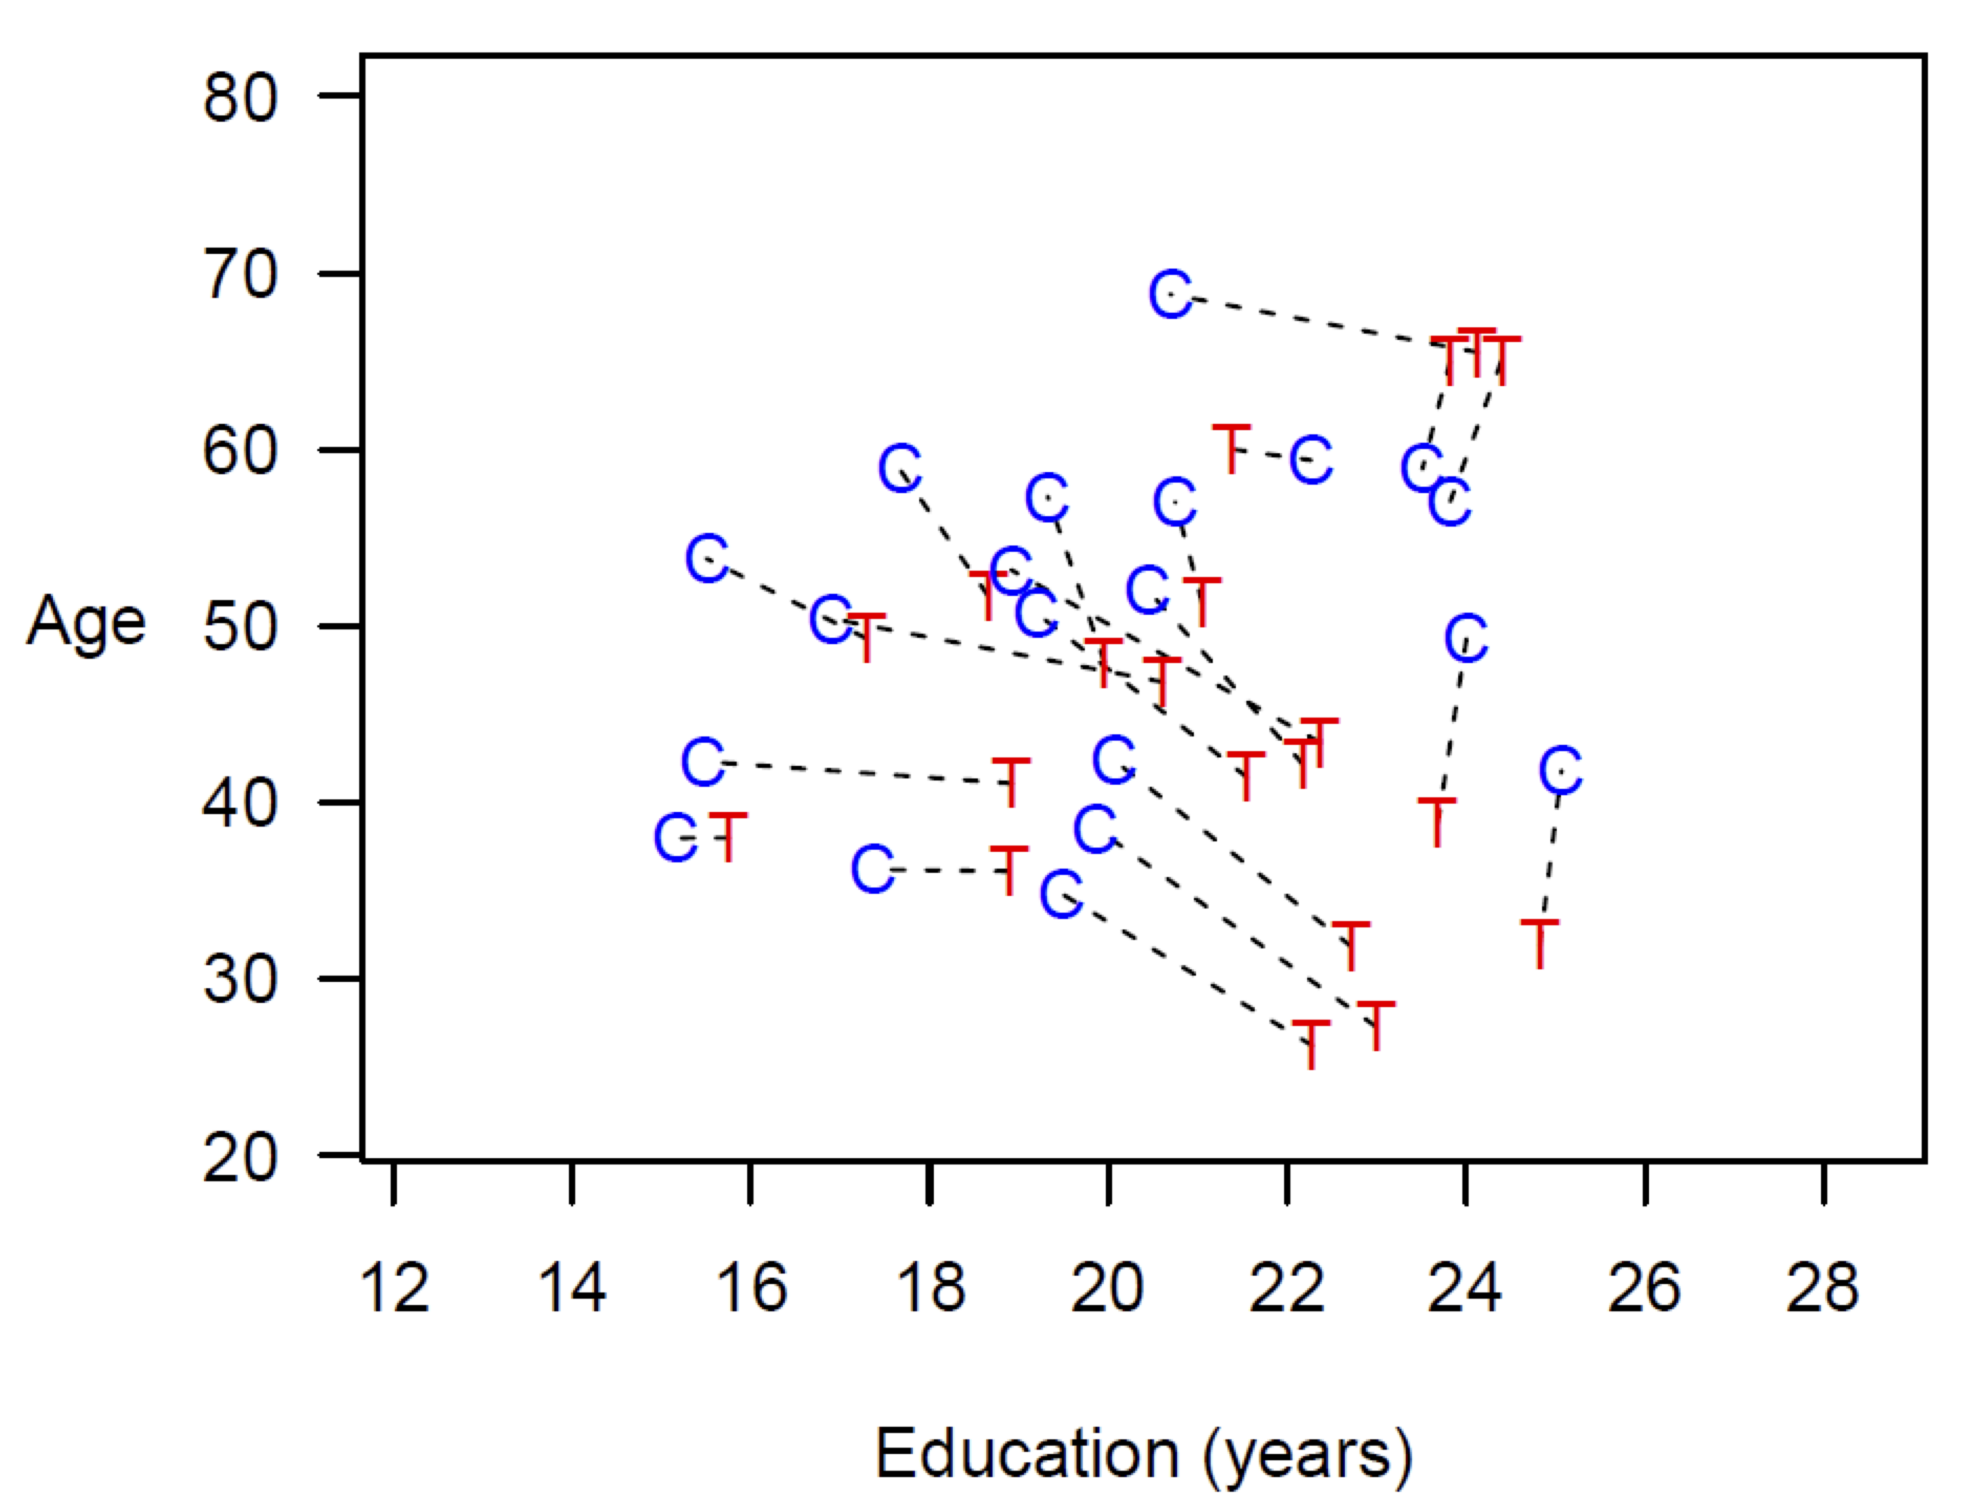
\includegraphics[width=0.7\textwidth]{figure/dm_f3.png}
		\end{figure}
		\begin{minipage}{0.9\linewidth}
			\fontsize{8}{8pt}\selectfont
			\emph{Source:} Ben Elsner's slides
		\end{minipage}
	\end{center}
\end{frame}


\begin{frame}{Distance Matching}{k-Nearest-neighbor Matching: k=10}
	\begin{center}
		\begin{figure}[p]
			\centering
			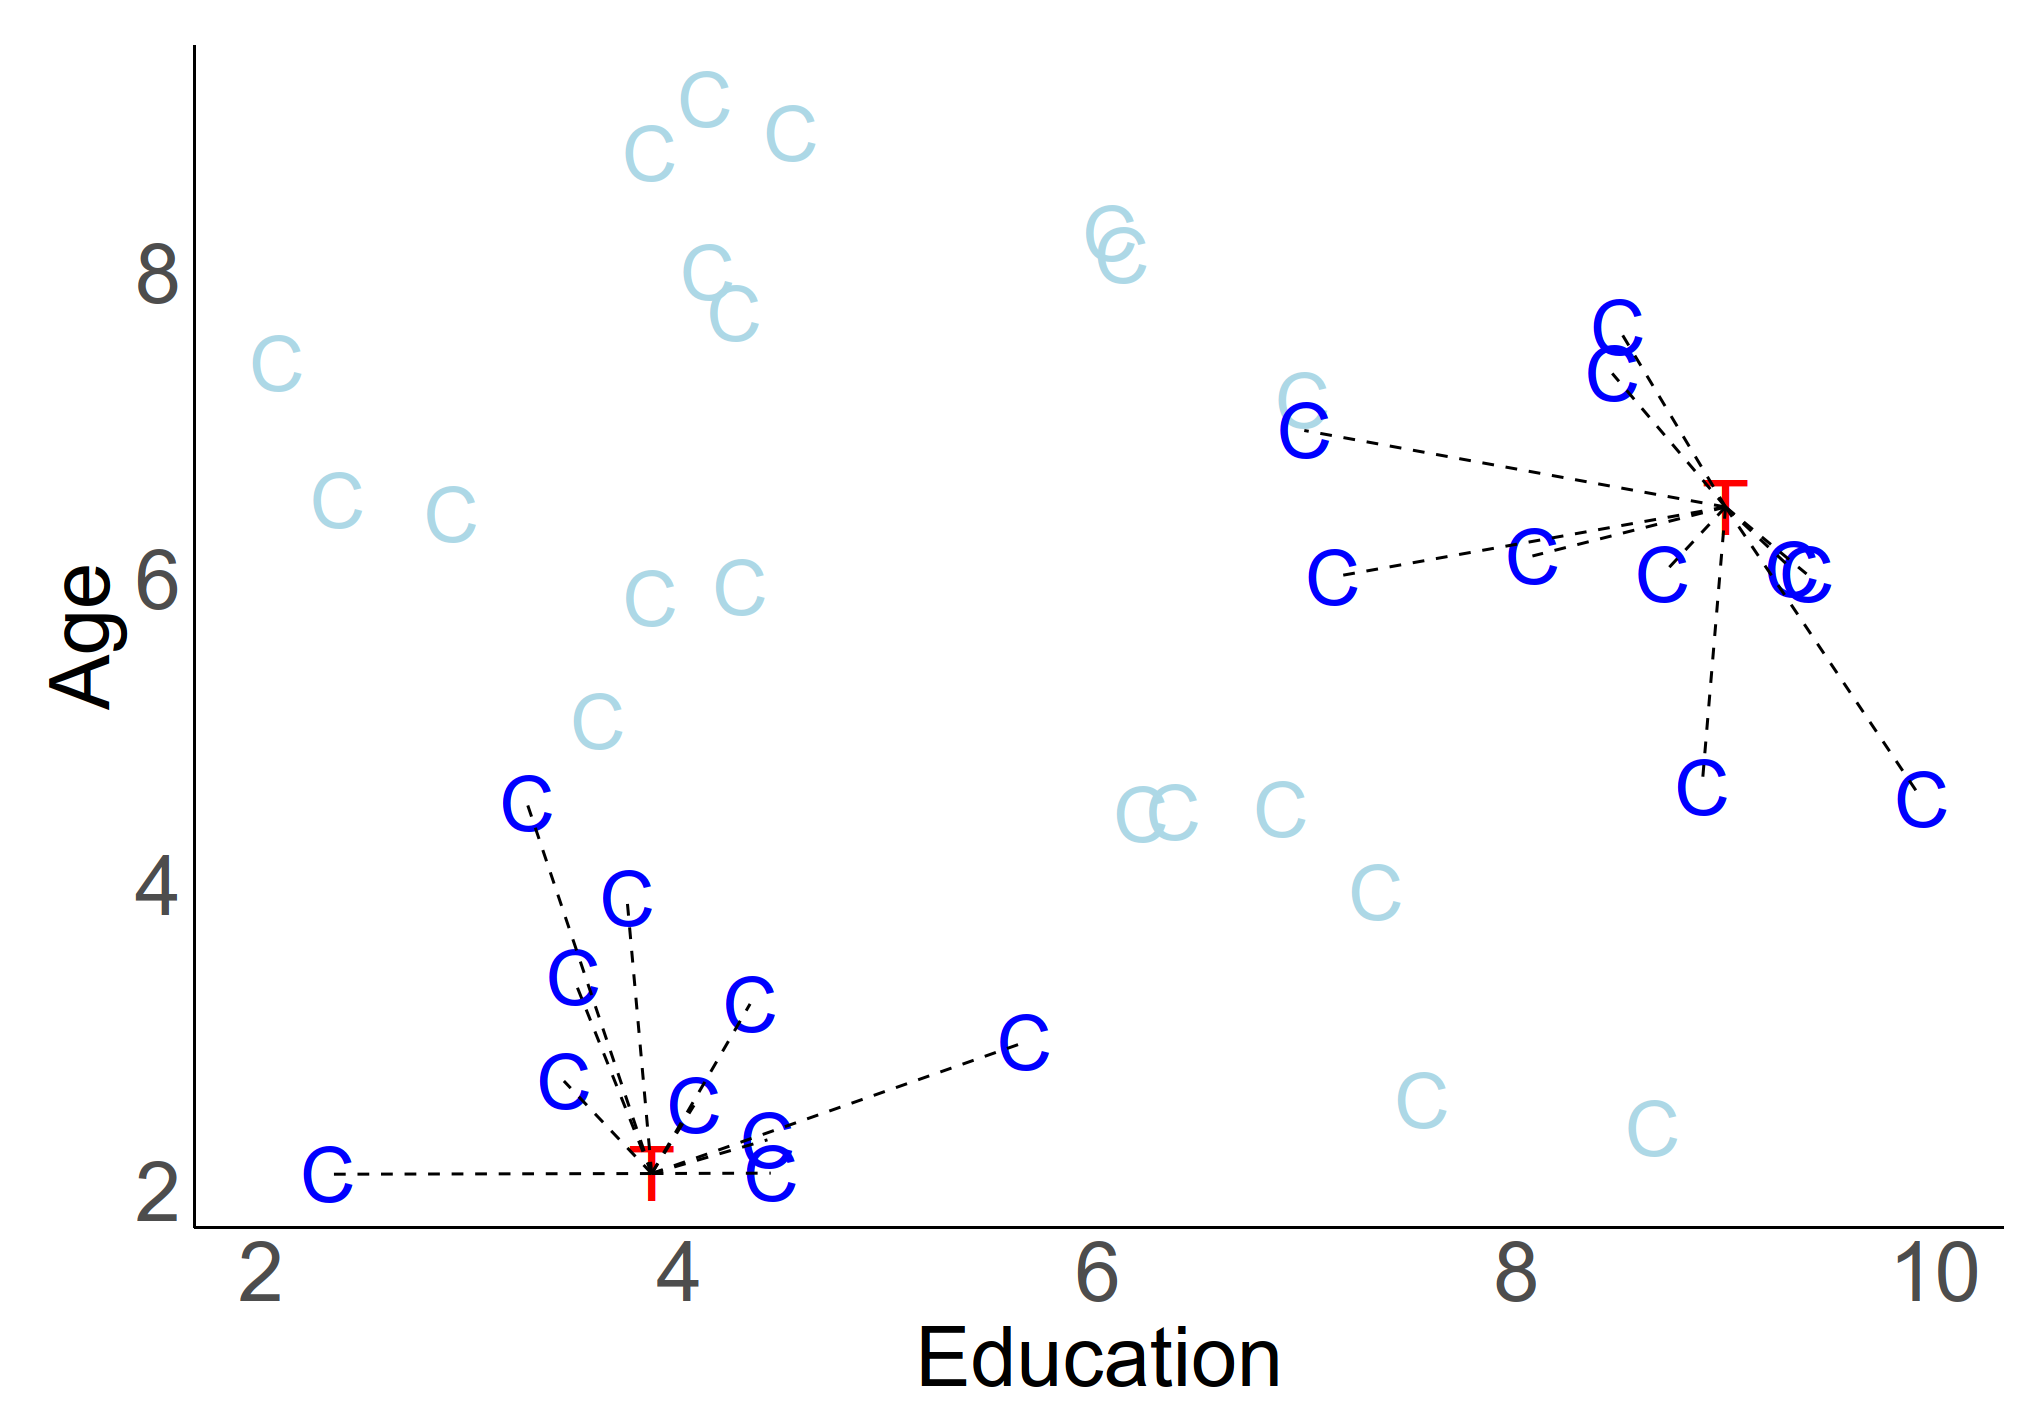
\includegraphics[width=0.7\textwidth]{figure/dm_f4.png}
		\end{figure}
		\begin{minipage}{0.9\linewidth}
			\fontsize{8}{8pt}\selectfont
			\emph{Source:} Ben Elsner's slides
		\end{minipage}
	\end{center}
\end{frame}


\begin{frame}{Distance Matching}{Radius Matching}
	\begin{center}
		\begin{figure}[p]
			\centering
			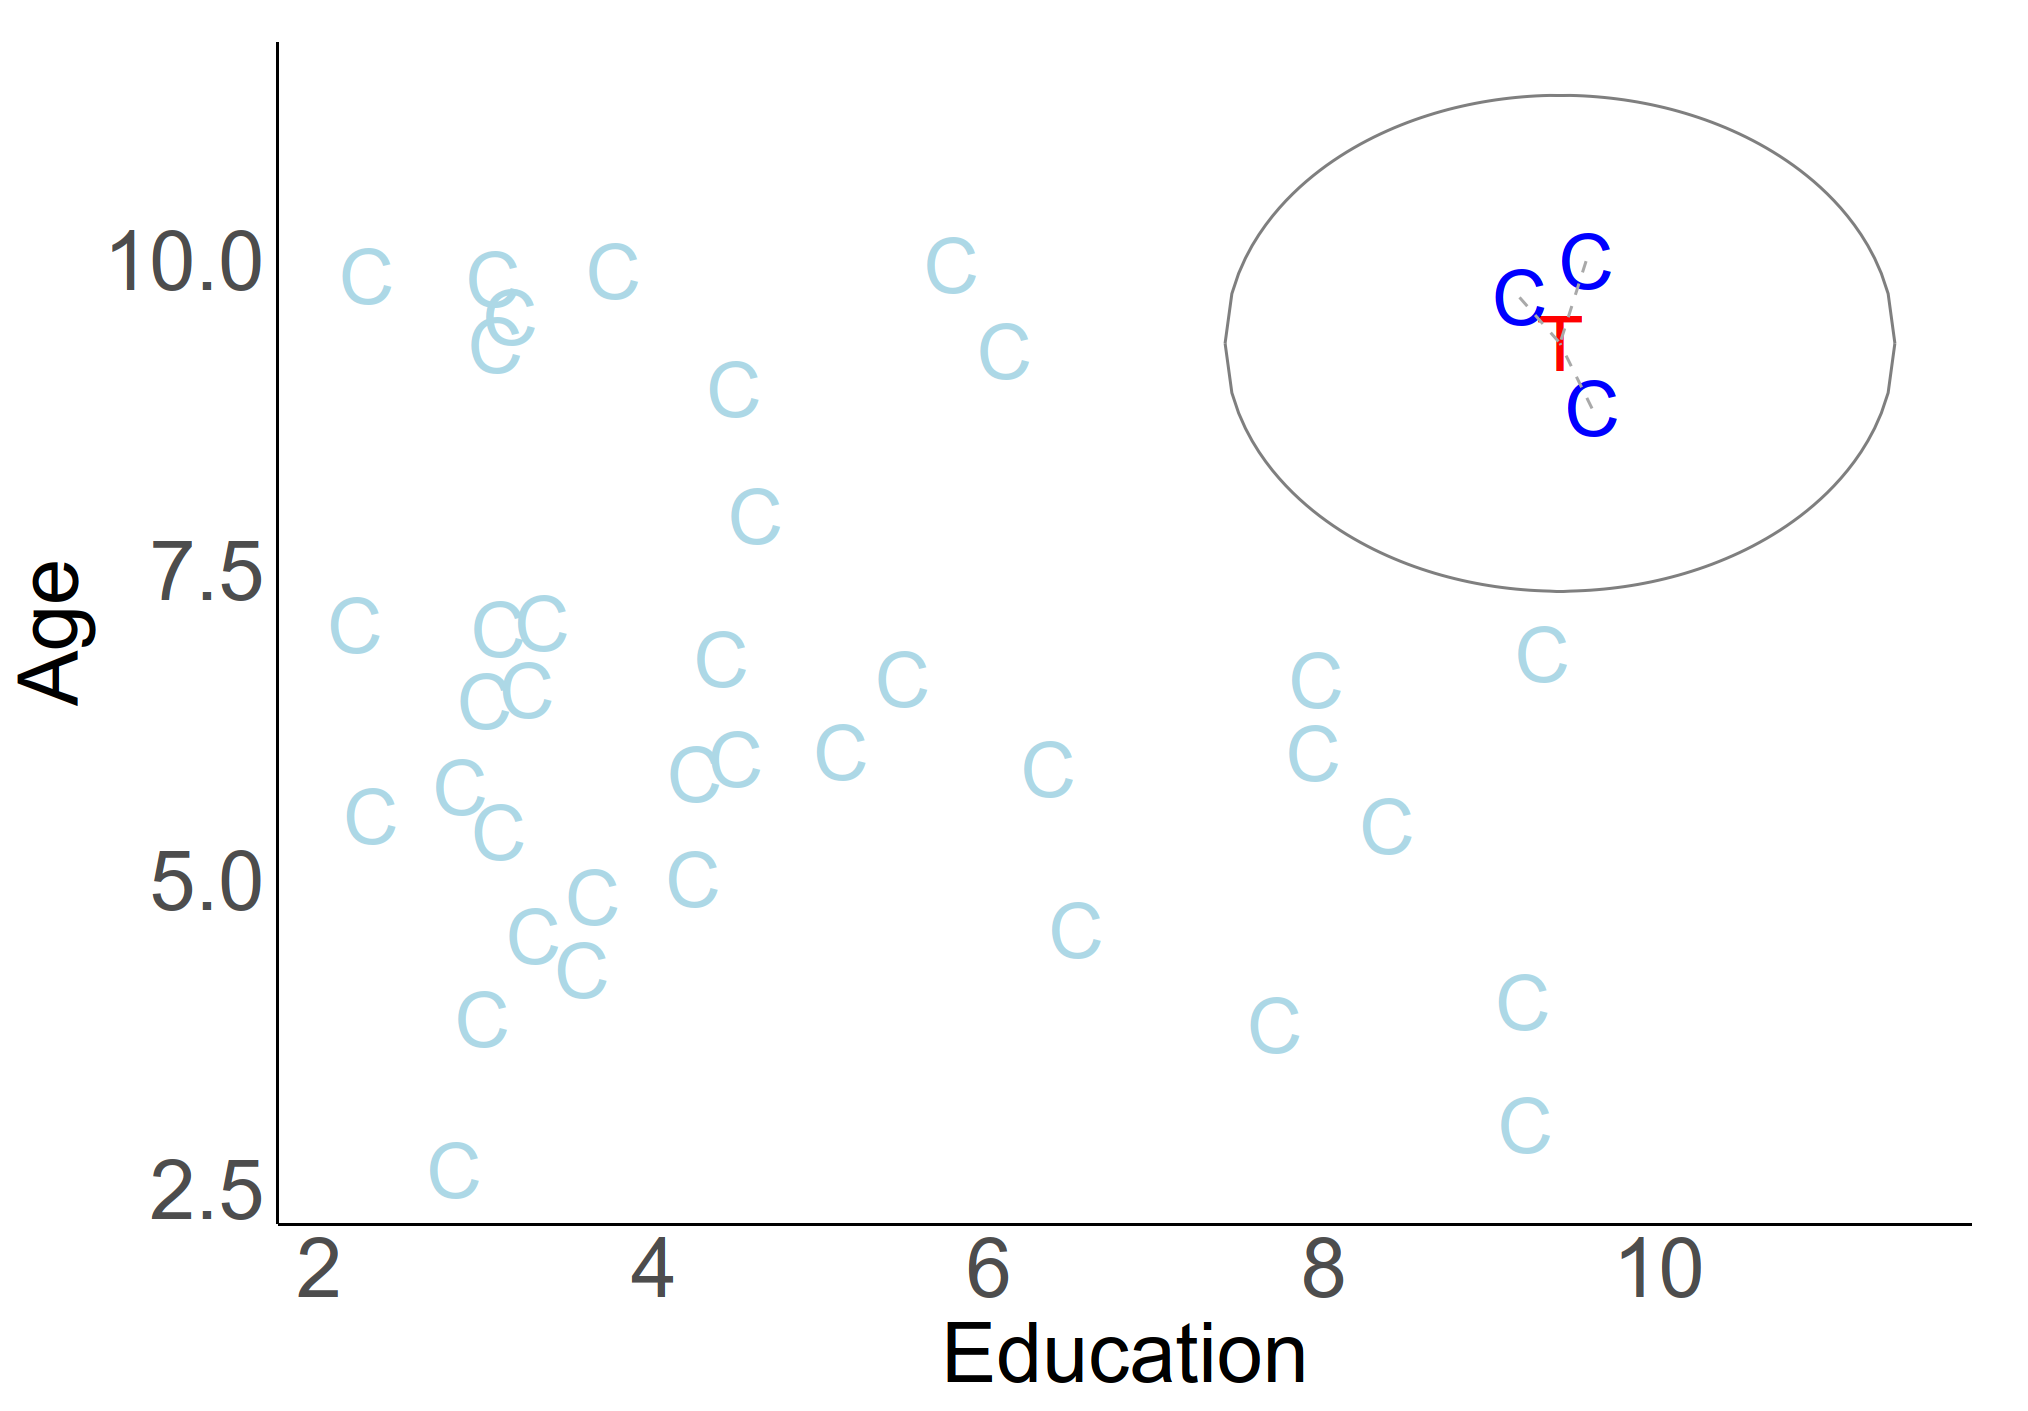
\includegraphics[width=0.7\textwidth]{figure/dm_f5.png}
		\end{figure}
		\begin{minipage}{0.9\linewidth}
			\fontsize{8}{8pt}\selectfont
			\emph{Source:} Ben Elsner's slides
		\end{minipage}
	\end{center}
\end{frame}


\begin{frame}{Matching and the ``Curse of Dimensionality"}
\begin{itemize}
\item Matching discrepancies $||X_i-X_{j(i)}||$ tend to increase with number of covariates, the dimension of $X$
\vspace{0.2cm}
\item It is difficult to find good matches in large dimensions: you need many observations if $H$ is large
\end{itemize}
\end{frame}


\title[]  
{Propensity Score Matching \\ Main Idea}

\author 
{}

\institute{}

\date
{}

\begin{frame}{}
\titlepage
\end{frame}


\begin{frame}{Propensity Score Matching}
\begin{itemize}
\item Instead of matching over $k$ dimensions, the method of \textbf{propensity score matching (PSM)} allows the matching
problem to be reduced to a single dimension
\vspace{0.2cm}
\begin{itemize}
\item The \textbf{propensity score} is defined as the treatment probability conditional on a set of observed variables $X_{i}$: 
	\begin{equation*}
	p(X_{i})=E[D_{i}|X_{i}]=Pr(D_{i}=1|X_{i})
	\end{equation*}

\item Intuitively, propensity score $p(X_{i})$ summarized all information of a set of covariates $X_{i}$ into a single value  
\vspace{0.2cm}
\item Then, we can just control (match) $p(X_{i})$ to eliminate selection bias
\end{itemize}
\end{itemize}
\end{frame}


\begin{frame}{Propensity Score Matching}
\begin{itemize}

\item Rosenbaum and Rubin (1983) proved that CIA (selection on observables) implies:
	\begin{equation*}
	(Y^{1}_{i},Y^{0}_{i})\indep D_{i}|p(X_{i})
	\end{equation*}
\begin{itemize}
\item Conditioning on the propensity score $p(X_{i})$ is enough to make treatment status be independent of the potential outcomes
\vspace{0.2cm}
\item Substantial dimension reduction in the matching variables!
\end{itemize}
\end{itemize}
\end{frame}


\begin{frame}{Propensity Score Matching}
\begin{itemize}

\begin{block}{Propensity Score Theorem}
Suppose the CIA holds, such that $ (\mathrm{Y}^{1}_{i},\mathrm{Y}^{0}_{i})\indep D_{i}|X_{i}$. Then $ (\mathrm{Y}^{1}_{i},\mathrm{Y}^{0}_{i})\indep D_{i}|p(X_{i})$
\end{block}

\item If potential outcomes are independent of treatment status
conditional on a set of covariates $X_{i}$
\vspace{0.2cm}
\item Then, potential outcomes are independent of treatment status $D_{i}$ conditional on the propensity score $p(X_{i})$
\end{itemize}
\end{frame}


\begin{frame}{Propensity Score Matching}
		\begin{itemize}
	\item Goal of Proof: 
	
	\begin{itemize}
	\item Assume that $ (\mathrm{Y}^{1}_{i},\mathrm{Y}^{0}_{i})\indep D_{i}|X_{i}$. Then:
		\vspace{0.2cm}
		\item[$\Rightarrow$] $Pr(D_{i}=1|\mathrm{Y}^{1}_{i},\mathrm{Y}^{0}_{i},p(X_{i}))=p(X_{i})=Pr(D_{i}=1|p(X_{i}))$
		\vspace{0.2cm}
		\item[$\Rightarrow$] $(\mathrm{Y}^{1}_{i},\mathrm{Y}^{0}_{i})\indep D_{i}|p(X_{i})$
	\end{itemize}
	
		\end{itemize}
\end{frame}


\begin{frame}{Propensity Score Matching}

Proof: Assume that $ (\mathrm{Y}^{1}_{i},\mathrm{Y}^{0}_{i})\indep D_{i}|X_{i}$. Then:
	\begin{equation*}
	\begin{aligned}
	Pr(D_{i}=1|\mathrm{Y}^{1}_{i},\mathrm{Y}^{0}_{i},p(X_{i}))
	&= E[D_{i}|\mathrm{Y}^{1}_{i},\mathrm{Y}^{0}_{i},p(X_{i})]\\
	&= E[E[D_{i}|\mathrm{Y}^{1}_{i},\mathrm{Y}^{0}_{i},p(X_{i}),X_{i}]|\mathrm{Y}^{1}_{i},\mathrm{Y}^{0}_{i},p(X_{i})]\\
	&= E[E[D_{i}|\mathrm{Y}^{1}_{i},\mathrm{Y}^{0}_{i},X_{i}]|\mathrm{Y}^{1}_{i},\mathrm{Y}^{0}_{i},p(X_{i})]\\
	&= E[E[D_{i}|X_{i}]|\mathrm{Y}^{1}_{i},\mathrm{Y}^{0}_{i},p(X_{i})]\\
	&= E[p(X_{i})|\mathrm{Y}^{1}_{i},\mathrm{Y}^{0}_{i},p(X_{i})] \\
	&= p(X_{i})
	\end{aligned}
	\end{equation*}

\end{frame}


\begin{frame}{Propensity Score Matching}
	
    Using a similar argument, we obtain
	\begin{equation*}
		\begin{aligned}
			Pr(D_{i}=1|p(X_{i}))
			&= E[D_{i}|p(X_{i})] \\
			&= E[E[D_{i}|p(X_{i}),X_{i}]|p(X_{i})]\\
			&= E[E[D_{i}|X_{i}]|p(X_{i})]\\
			&= E[p(X_{i})|p(X_{i})] \\
			&= p(X_{i})
		\end{aligned}
	\end{equation*}
	\begin{itemize}
		\item[$\Rightarrow$] $Pr(D_{i}=1|\mathrm{Y}^{1}_{i},\mathrm{Y}^{0}_{i},p(X_{i}))=p(X_{i})=Pr(D_{i}=1|p(X_{i}))$
		\item[$\Rightarrow$] $(\mathrm{Y}^{1}_{i},\mathrm{Y}^{0}_{i})\indep D_{i}|p(X_{i})$
	\end{itemize}
\end{frame}


\begin{frame}{Propensity Score Matching}
	\begin{itemize}
		\item From CIA, to get causal effect, we need only control for covariates that affect the probability of treatment
		\vspace{0.2cm}
		\item The propensity score theorem says something more: 
				\vspace{0.2cm}
			\begin{itemize}
		\item \textbf{The only covariate you really need to control for is the probability of treatment itself $p(X_{i}) = Pr(D_{i}=1|X_{i}) $}
			\end{itemize}
	\end{itemize}
\end{frame}


% -------------------------------------------------------
% Identification Results: Road Map (PSM)
% -------------------------------------------------------

\begin{frame}{Identification Results for PSM}
	\begin{itemize}
		\item PSM follows the same three identification steps as matching, but conditions on $p(X_i)$ instead of $X_i$:
		\vspace{0.3cm}
		\begin{itemize}
			\item[\textbf{Step 1}] Show that ODO at given $p(X_i)$ equals \textbf{CATT} (selection bias = 0)
			\vspace{0.2cm}
			\item[\textbf{Step 2}] Under CIA, CATT = CATU = \textbf{CATE}
			\vspace{0.2cm}
			\item[\textbf{Step 3}] Apply LIE to average CATE over $p(X)$ $\Rightarrow$ \textbf{ATT, ATU, ATE}
		\end{itemize}
	\end{itemize}
\end{frame}


% -------------------------------------------------------
% Steps 1 & 2
% -------------------------------------------------------

\begin{frame}{Identification Results for PSM}{Steps 1 \& 2: ODO = CATT = CATU = CATE}
{\small
\begin{equation*}
\begin{aligned}
&
\underbrace{\mathrm{E}[\mathrm{Y}_{i}|p(X_{i}),D_{i}=1] - \mathrm{E}[\mathrm{Y}_{i}|p(X_{i}),D_{i}=0]}_{\text{ODO at given } p(X_{i})}  \\
&=\mathrm{E}[\mathrm{Y}^{1}_{i}|p(X_{i}),D_{i}=1] - \mathrm{E}[\mathrm{Y}^{0}_{i}|p(X_{i}),D_{i}=0] \\
&= \mathrm{E}[\mathrm{Y}^{1}_{i}|p(X_{i}),D_i=1]-{\color{red} \mathrm{E}[\mathrm{Y}^{0}_{i}|p(X_{i}),D_i=1]} \\
&\quad + {\color{red} \mathrm{E}[\mathrm{Y}^{0}_{i}|p(X_{i}),D_i=1]}-\mathrm{E}[\mathrm{Y}^{0}_{i}|p(X_{i}),D_i=0] \\
&= \underbrace{\mathrm{E}[\mathrm{Y}^{1}_{i}-\mathrm{Y}^{0}_{i}|p(X_{i}),D_i=1]}_{\text{CATT}}
+ \underbrace{\mathrm{E}[\mathrm{Y}^{0}_{i}|p(X_{i}),D_i=1]-\mathrm{E}[\mathrm{Y}^{0}_{i}|p(X_{i}),D_i=0]}_{\scriptstyle\text{Selection Bias} = 0 \text{ by CIA}}  \\
&= \underbrace{\mathrm{E}[\mathrm{Y}^{1}_{i}-\mathrm{Y}^{0}_{i}|p(X_{i}),D_i=0]}_{\text{CATU}} \quad \text{(by CIA)}
= \underbrace{\mathrm{E}[\mathrm{Y}^{1}_{i}-\mathrm{Y}^{0}_{i}|p(X_{i})]}_{\text{CATE}}
\end{aligned}
\end{equation*}
}
\end{frame}


% -------------------------------------------------------
% Step 3: ATT, ATU, ATE (concise)
% -------------------------------------------------------

\begin{frame}{Identification Results for PSM}{Step 3: ATT, ATU, and ATE}
	\begin{itemize}

		\item \textbf{ATT}: average CATT over the \textbf{treatment group} distribution of $p(X)$:
		\begin{equation*}
			\mathrm{E}\Big[\underbrace{\mathrm{E}[\mathrm{Y}^{1}_{i}-\mathrm{Y}^{0}_{i}|p(X_{i}),D_i=1]}_{\text{CATT}}\Big| D_i=1\Big]
			=\underbrace{\mathrm{E}[\mathrm{Y}^{1}_{i}-\mathrm{Y}^{0}_{i}|D_i=1]}_{\text{ATT}}
		\end{equation*}

		\vspace{0.1cm}
		\item \textbf{ATU}: average CATU over the \textbf{control group} distribution of $p(X)$:
		\begin{equation*}
			\mathrm{E}\Big[\underbrace{\mathrm{E}[\mathrm{Y}^{1}_{i}-\mathrm{Y}^{0}_{i}|p(X_{i}),D_i=0]}_{\text{CATU}}\Big| D_i=0\Big]
			=\underbrace{\mathrm{E}[\mathrm{Y}^{1}_{i}-\mathrm{Y}^{0}_{i}|D_i=0]}_{\text{ATU}}
		\end{equation*}

		\vspace{0.1cm}
		\item \textbf{ATE}: average CATE over the \textbf{full population} distribution of $p(X)$:
		\begin{equation*}
			\mathrm{E}\Big[\underbrace{\mathrm{E}[\mathrm{Y}^{1}_{i}-\mathrm{Y}^{0}_{i}|p(X_{i})]}_{\text{CATE}}\Big]
			=\underbrace{\mathrm{E}[\mathrm{Y}^{1}_{i}-\mathrm{Y}^{0}_{i}]}_{\text{ATE}}
		\end{equation*}

		\vspace{0.1cm}
		\item \textbf{Summary}: Under CIA, PSM can identify ATT, ATU, and ATE by averaging $p(X)$-specific effects over the appropriate population

	\end{itemize}
\end{frame}


\title[]  
{Propensity Score Matching \\ Estimation}

\author 
{}

\institute{}

\date
{}

\begin{frame}{}
\titlepage
\end{frame}


\begin{frame}{Propensity Score Matching}{Estimation}
	\begin{itemize}
		\item There are two ways to estimate causal effect of treatment using PSM
			\vspace{0.2cm}
			\begin{itemize}	
		\item[1] Nearest Neighbor: 
		
			\begin{itemize}
							\vspace{0.2cm}
		\item By matching each treated observation to the untreated observation with the same or similar values of the propensity score
					\end{itemize}
					\vspace{0.2cm}
		\item[2] Weighting Approach
		\begin{itemize}
			\vspace{0.2cm}
			\item Skip the cumbersome matching procedure and re-weight sample
		\end{itemize}
				
			\end{itemize}
	\end{itemize}
\end{frame}


\begin{frame}{Propensity Score Matching}{Estimation: Nearest Neighbor}
	\begin{itemize}
		\item There are two steps to estimate causal effect of treatment using PSM with nearest neighbor
		\vspace{0.2cm}
		\begin{itemize}
			\item[1] Estimate the propensity score: $\hat{p}(X)=\hat{Pr}(D_{i}=1|X_{i})$  using logit or porbit regression
			
	
		\begin{eqnarray*}
			D_{i} = \beta_{0}  + \beta_{1} X^{1}_{i}  + \beta_{2} X^{2}_{i}  + ...... + \beta_{h} X^{h}_{i}  + \epsilon_{i}
		\end{eqnarray*}	
			
			
			\item[2] By matching each treated observation
			to the observation (control group) with the same or similar values of the propensity score $\hat{Pr}(D_{i}=1|X_{i})$
		\end{itemize}
		
	\end{itemize}
\end{frame}


\begin{frame}{Propensity Score Matching}{A Numerical Example}
	\begin{center}
		\scalebox{0.75}{
			\begin{threeparttable}
				\centering\footnotesize
				\begin{tabular}{@{} ccrccrccr @{}}
					\multicolumn{3}{c}{Trainees} & \multicolumn{3}{c}{Non-Trainees} & \multicolumn{3}{c}{Matched Sample}\\
					\cmidrule(l){1-3}  \cmidrule(l){4-6} \cmidrule(l){7-9} 
					unit   & pro-score   & earnings   & unit   & pro-score   & earnings  & unit  & pro-score  & earnings \\
					1 & 0.28 & 17700 &  1 & 0.43 & 20900 &    &  &   \\
					2 & 0.34 & 10200 &  2 & 0.50 & 31000 &    &  &   \\ 
					3 & 0.29 & 14400 &  3 & 0.30 & 21000 &    &  &   \\ 
					4 & 0.25 & 20800 &  4 & 0.27 & 9300  &    &  &   \\  
					5 & 0.29 & 6100  &  5 & 0.54 & 41100 &    &  &   \\
					7 & 0.33 & 21900 &  7 & 0.39 & 42000 &    &  &   \\
					8 & 0.27 & 28800 &  8 & 0.28 & 8800  &    &  &   \\  
					9 & 0.31 & 20300 &  9 & 0.24 & 25500 &    &  &   \\  
					10 & 0.26 & 28100 & 10 & 0.33 & 15500 & {\color{white}11,13}   &  &   \\
					11 & 0.25 & 9400  & 11 & 0.26 & 400   &    &  &   \\
					12 & 0.27 & 14300 & 12 & 0.31 & 26600 &    &  &   \\
					13 & 0.29 & 12500 & 13 & 0.26 & 16500 &    &  &   \\
					14 & 0.24 & 19700 & 14 & 0.34 & 24200 &    &  &   \\
					15 & 0.25 & 10100 & 15 & 0.25 & 23300 &    &  &   \\
					16 & 0.43 & 10700 & 16 & 0.24 & 9700  &    &  &   \\ 
					17 & 0.28 & 11500 & 17 & 0.29 & 6200  &    &  &   \\ 
					18 & 0.27 & 10700 & 18 & 0.35 & 30200 &    &  &   \\
					19 & 0.28 & 16300 & 19 & 0.32 & 17800 &    &  &   \\ 
					&    &       & 20 & 23 & 9500  &    &  &   \\
					&    &       & 21 & 32 & 25900 &    &  &   \\ 
					\cmidrule(l){1-3}  \cmidrule(l){4-6} \cmidrule(l){7-9} 
					Avg: &  & 16426 & Avg: &  & 20724 & Avg: & {\color{white}28.5} &  \\
				\end{tabular}
		\end{threeparttable}}
	\end{center}
\end{frame}


\begin{frame}{Propensity Score Matching}{A Numerical Example}
	\begin{center}
	\scalebox{0.75}{
			\begin{threeparttable}
				\centering\footnotesize
				\begin{tabular}{@{} ccrccrccr @{}}
					\multicolumn{3}{c}{Trainees} & \multicolumn{3}{c}{Non-Trainees} & \multicolumn{3}{c}{Matched Sample}\\
					\cmidrule(l){1-3}  \cmidrule(l){4-6} \cmidrule(l){7-9} 
					unit   & pro-score   & earnings   & unit   & pro-score   & earnings  & unit  & pro-score   & earnings \\
					1 & 0.28 & 17700 &  1 & 0.43 & 20900 &  8 & 0.28 & 8800   \\
					2 & 0.34 & 10200 &  2 & 0.50 & 31000 & 14 & 0.34 & 24200  \\ 
					3 & 0.29 & 14400 &  3 & 0.30 & 21000 & 17 & 0.29 & 6200   \\ 
					4 & 0.25 & 20800 &  4 & 0.27 & 9300  & 15 & 0.25 & 23300  \\  
					5 & 0.29 & 6100  &  5 & 0.54 & 41100 & 17 & 0.29 & 6200   \\
					6 & 0.23 & 28600 &  6 & 0.48 & 29800 & 20 & 0.23 & 9500   \\
					7 & 0.33 & 21900 &  7 & 0.39 & 42000 & 10 & 0.33 & 15500  \\
					8 & 0.27 & 28800 &  8 & 0.28 & 8800  &  4 & 0.27 & 9300   \\  
					9 & 0.31 & 20300 &  9 & 0.24 & 25500 & 12 & 0.31 & 26600  \\  
					10 & 0.26 & 28100 & 10 & 0.33 & 15500 & 11,13 & 0.26 & 8450   \\
					11 & 0.25 & 9400  & 11 & 0.26 & 400   & 15 & 0.25 & 23300  \\
					12 & 0.27 & 14300 & 12 & 0.31 & 26600 &  4 & 0.27 & 9300   \\
					13 & 0.29 & 12500 & 13 & 0.26 & 16500 & 17 & 0.29 & 6200   \\
					14 & 0.24 & 19700 & 14 & 0.34 & 24200 & 9,16 & 0.24 & 17700  \\
					15 & 0.25 & 10100 & 15 & 0.25 & 23300 & 15 & 0.25 & 23300  \\
					16 & 0.43 & 10700 & 16 & 0.24 & 9700  &  1 & 0.43 & 20900  \\ 
					17 & 0.28 & 11500 & 17 & 0.29 & 6200  &  8 & 0.28 & 8800   \\ 
					18 & 0.27 & 10700 & 18 & 0.35 & 30200 &  4 & 0.27 & 9300   \\
					19 & 0.28 & 16300 & 19 & 0.32 & 17800 &  8 & 0.28 & 8800  \\ 
					&    &       & 20 & 0.23 & 9500  &    &  &   \\
					&    &       & 21 & 0.32 & 25900 &    &  &   \\ 
					\cmidrule(l){1-3}  \cmidrule(l){4-6} \cmidrule(l){7-9} 
					Avg: &  & 16426 & Avg: &  & 20724 & Avg: &  & 13982 \\
				\end{tabular}
		\end{threeparttable}}
	\end{center}
\end{frame}


\begin{frame}{Propensity Score Matching}{A Numerical Example}
	\begin{center}
		\begin{figure}[p]
			\centering
			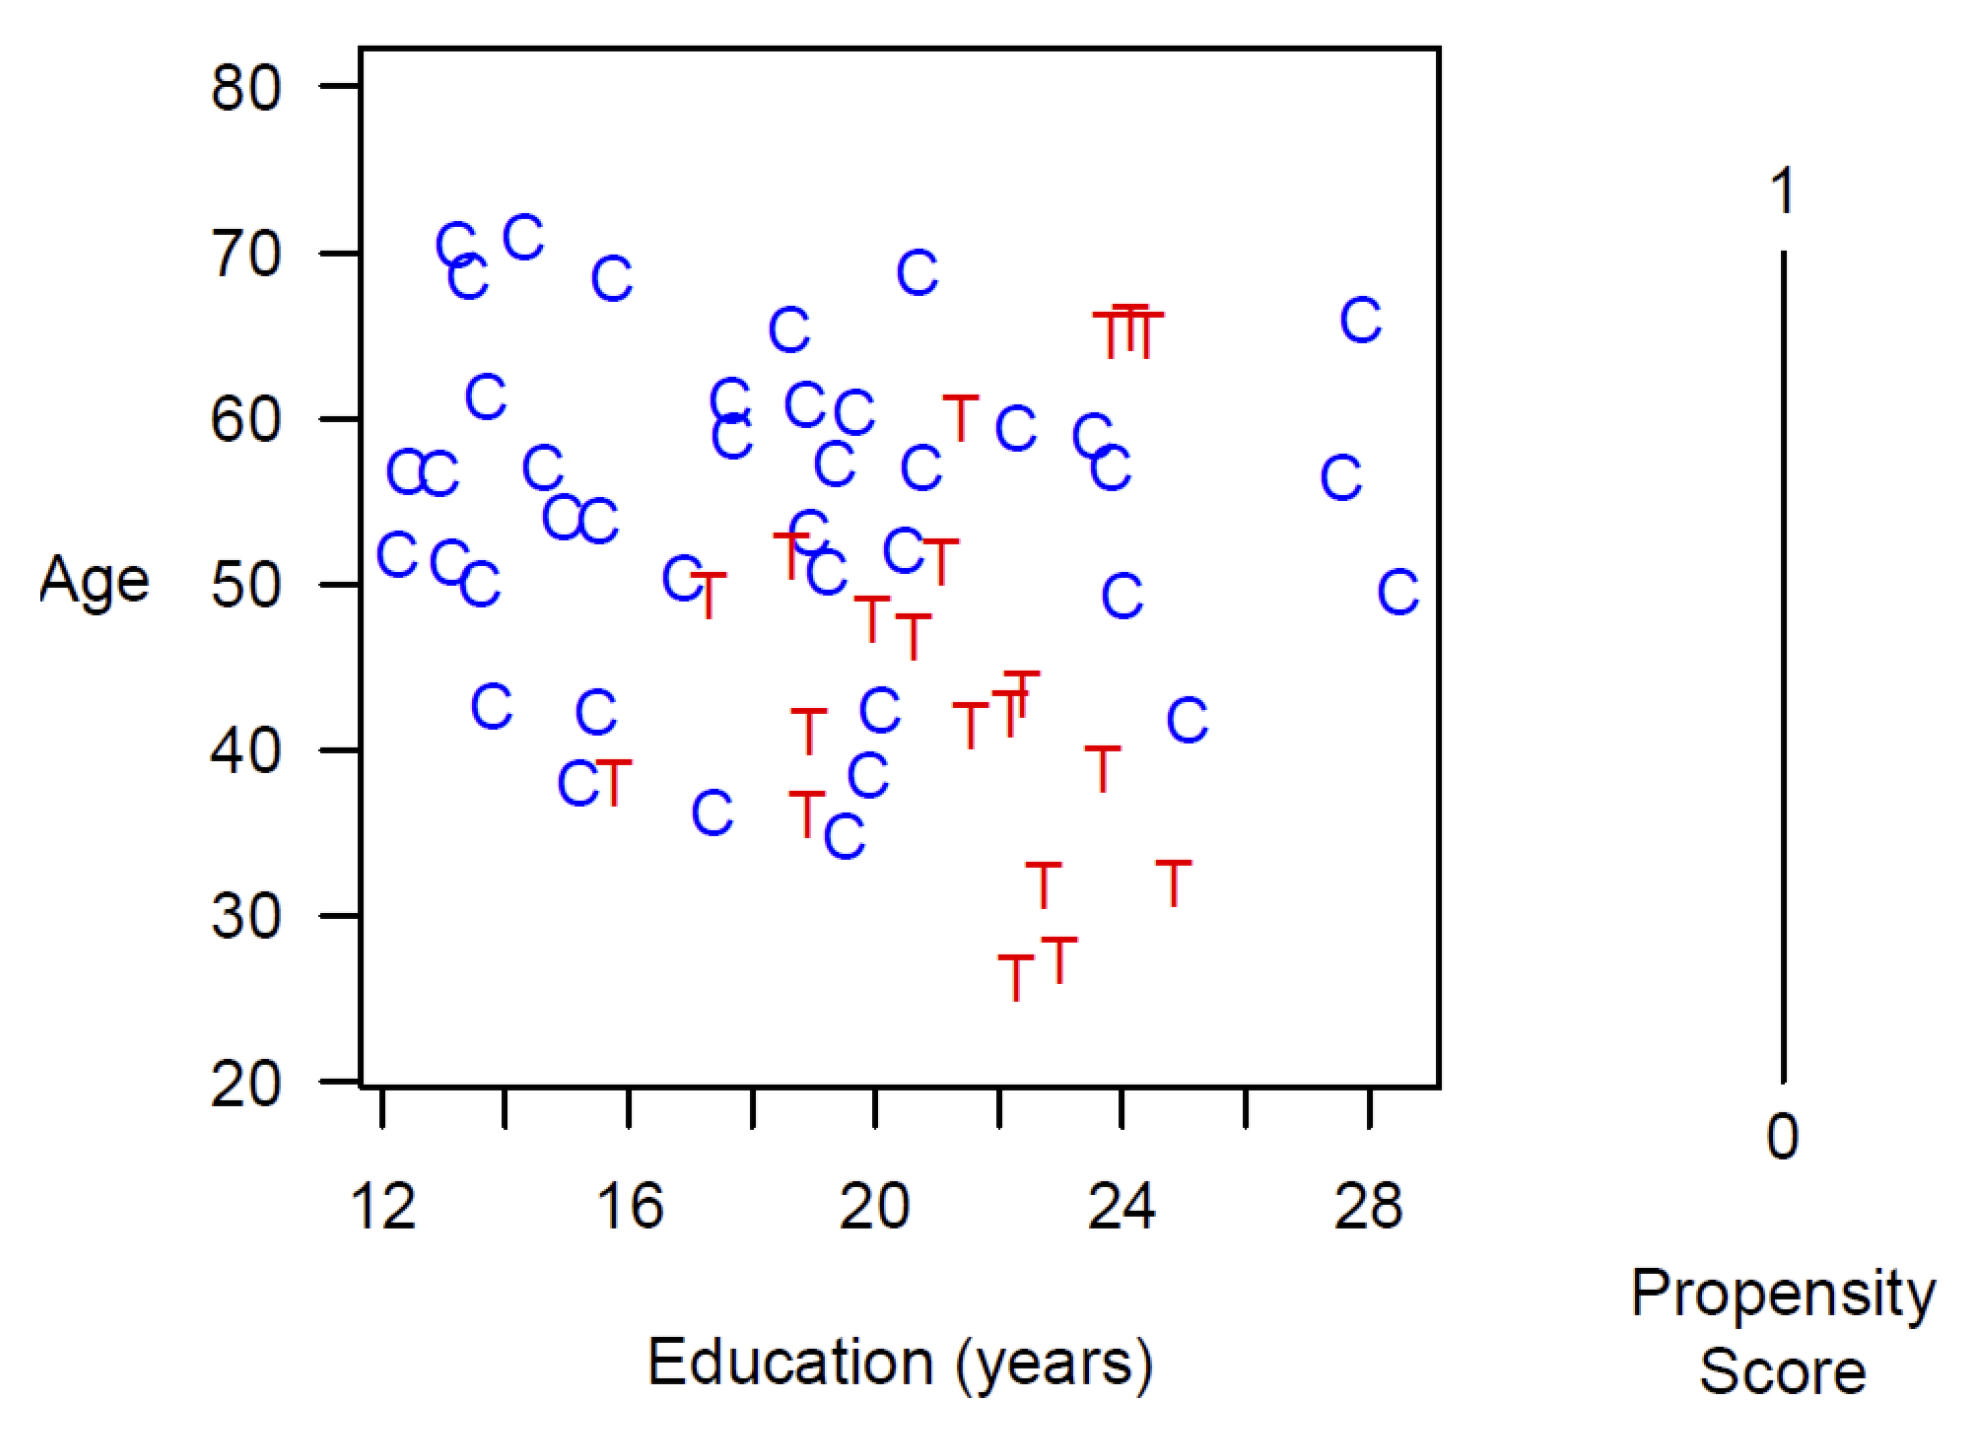
\includegraphics[width=0.7\textwidth]{figure/psm_f1.png}
		\end{figure}
		\begin{minipage}{0.9\linewidth}
			\fontsize{8}{8pt}\selectfont
			\emph{Source:} Ben Elsner's slides
		\end{minipage}
	\end{center}
\end{frame}


\begin{frame}{Propensity Score Matching}{A Numerical Example}
	\begin{center}
		\begin{figure}[p]
			\centering
			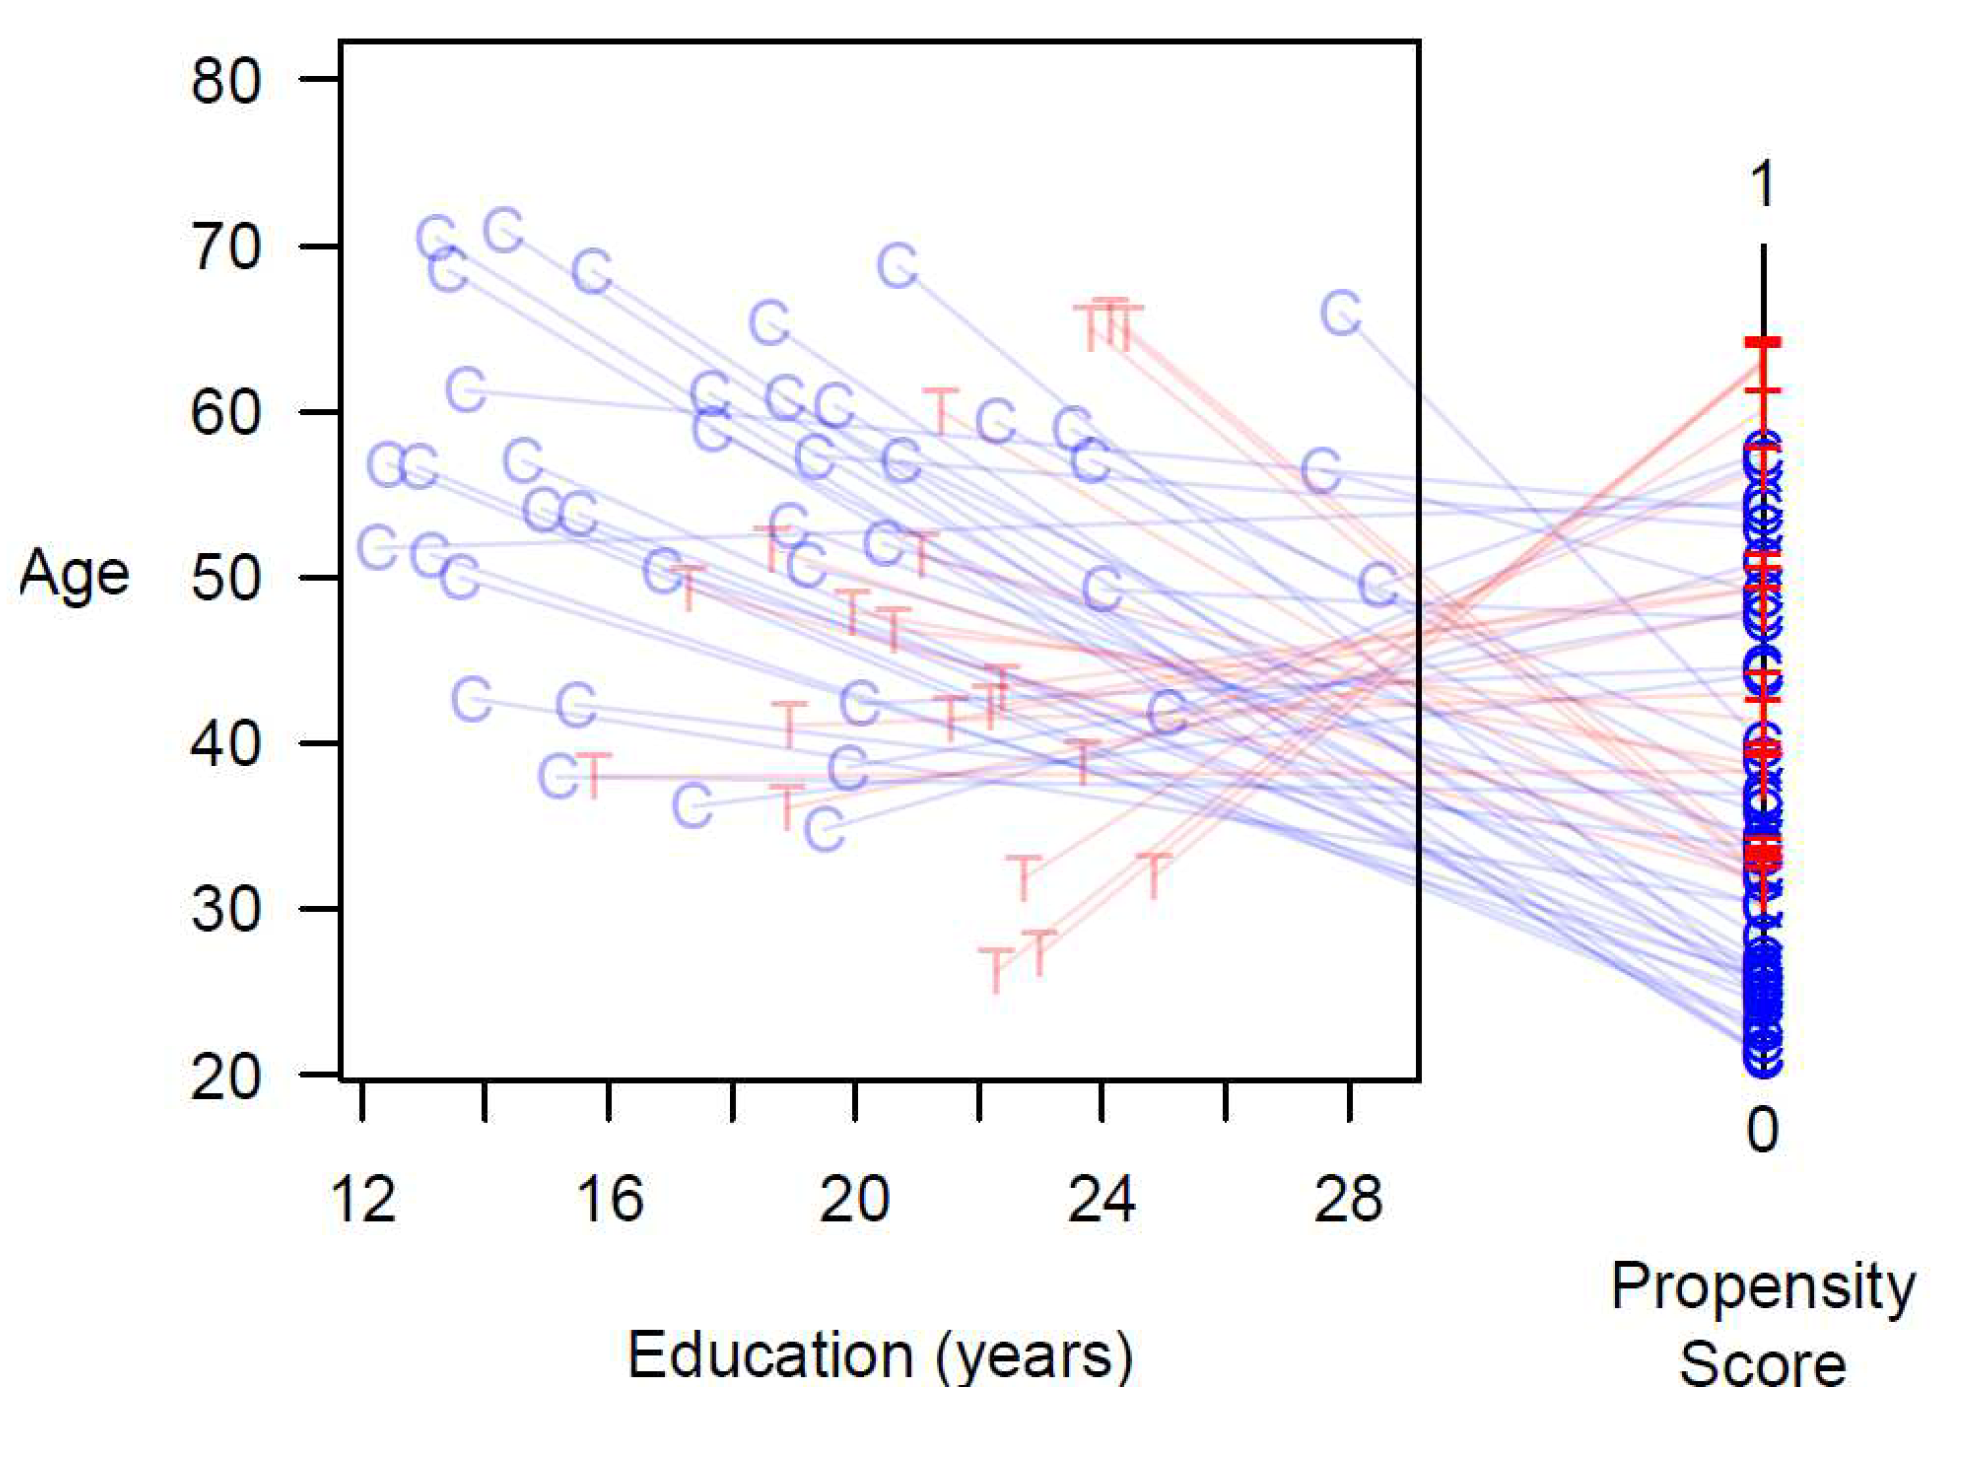
\includegraphics[width=0.7\textwidth]{figure/psm_f2.png}
		\end{figure}
		\begin{minipage}{0.9\linewidth}
			\fontsize{8}{8pt}\selectfont
			\emph{Source:} Ben Elsner's slides
		\end{minipage}
	\end{center}
\end{frame}


\begin{frame}{Propensity Score Matching}{A Numerical Example}
	\begin{center}
		\begin{figure}[p]
			\centering
			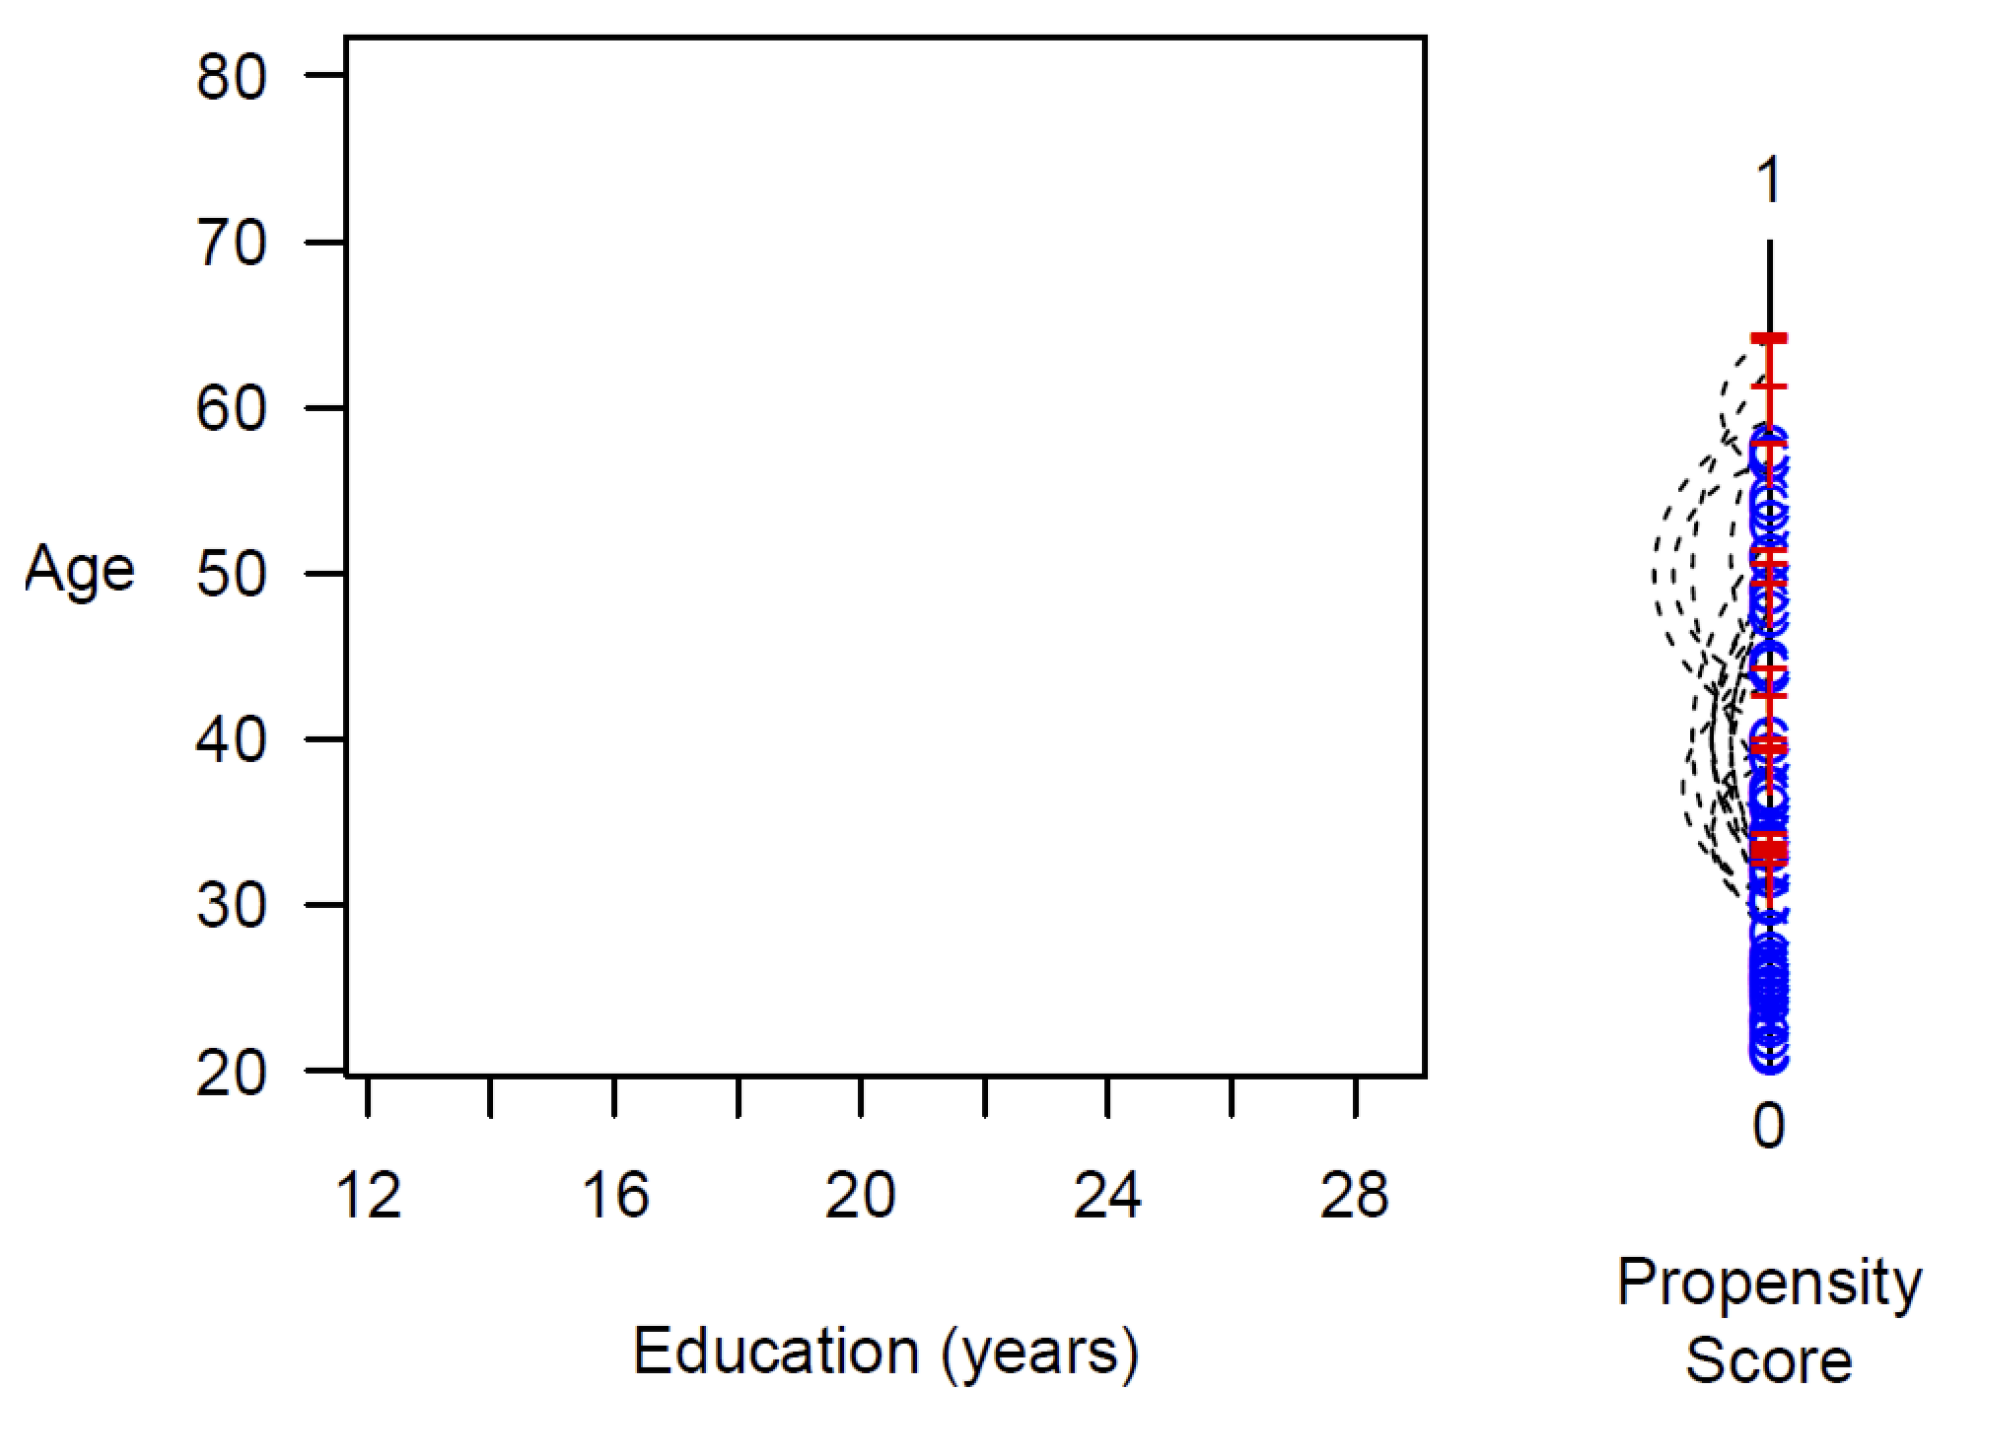
\includegraphics[width=0.7\textwidth]{figure/psm_f3.png}
		\end{figure}
		\begin{minipage}{0.9\linewidth}
			\fontsize{8}{8pt}\selectfont
			\emph{Source:} Ben Elsner's slides
		\end{minipage}
	\end{center}
\end{frame}


\begin{frame}{Propensity Score Matching}{A Numerical Example}
	\begin{center}
		\begin{figure}[p]
			\centering
			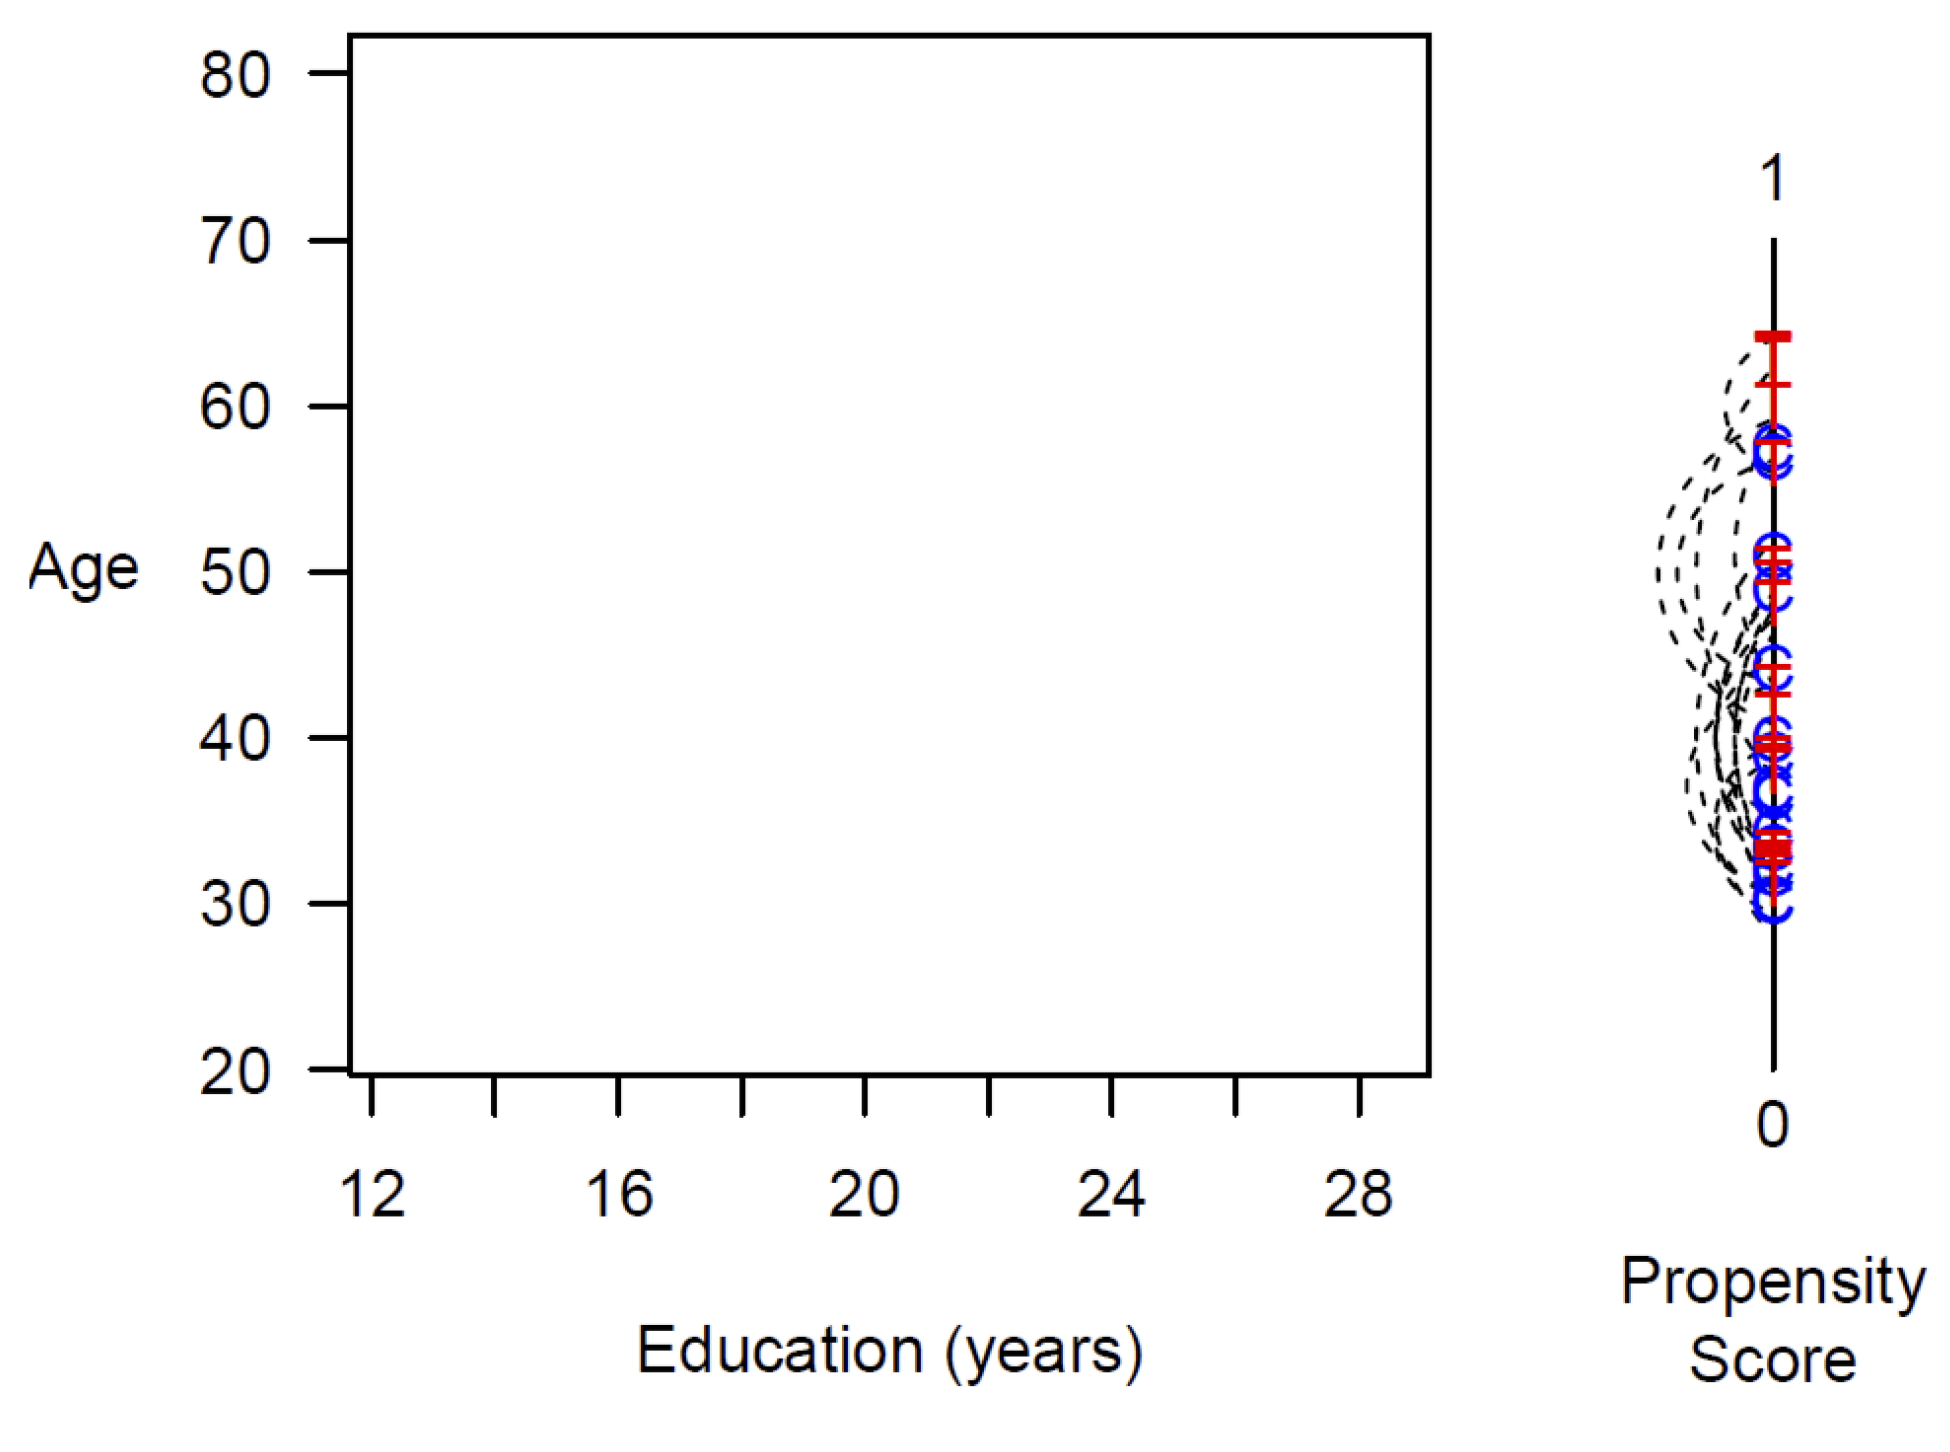
\includegraphics[width=0.7\textwidth]{figure/psm_f4.png}
		\end{figure}
		\begin{minipage}{0.9\linewidth}
			\fontsize{8}{8pt}\selectfont
			\emph{Source:} Ben Elsner's slides
		\end{minipage}
	\end{center}
\end{frame}


\begin{frame}{Propensity Score Matching}{A Numerical Example}
	\begin{center}
		\begin{figure}[p]
			\centering
			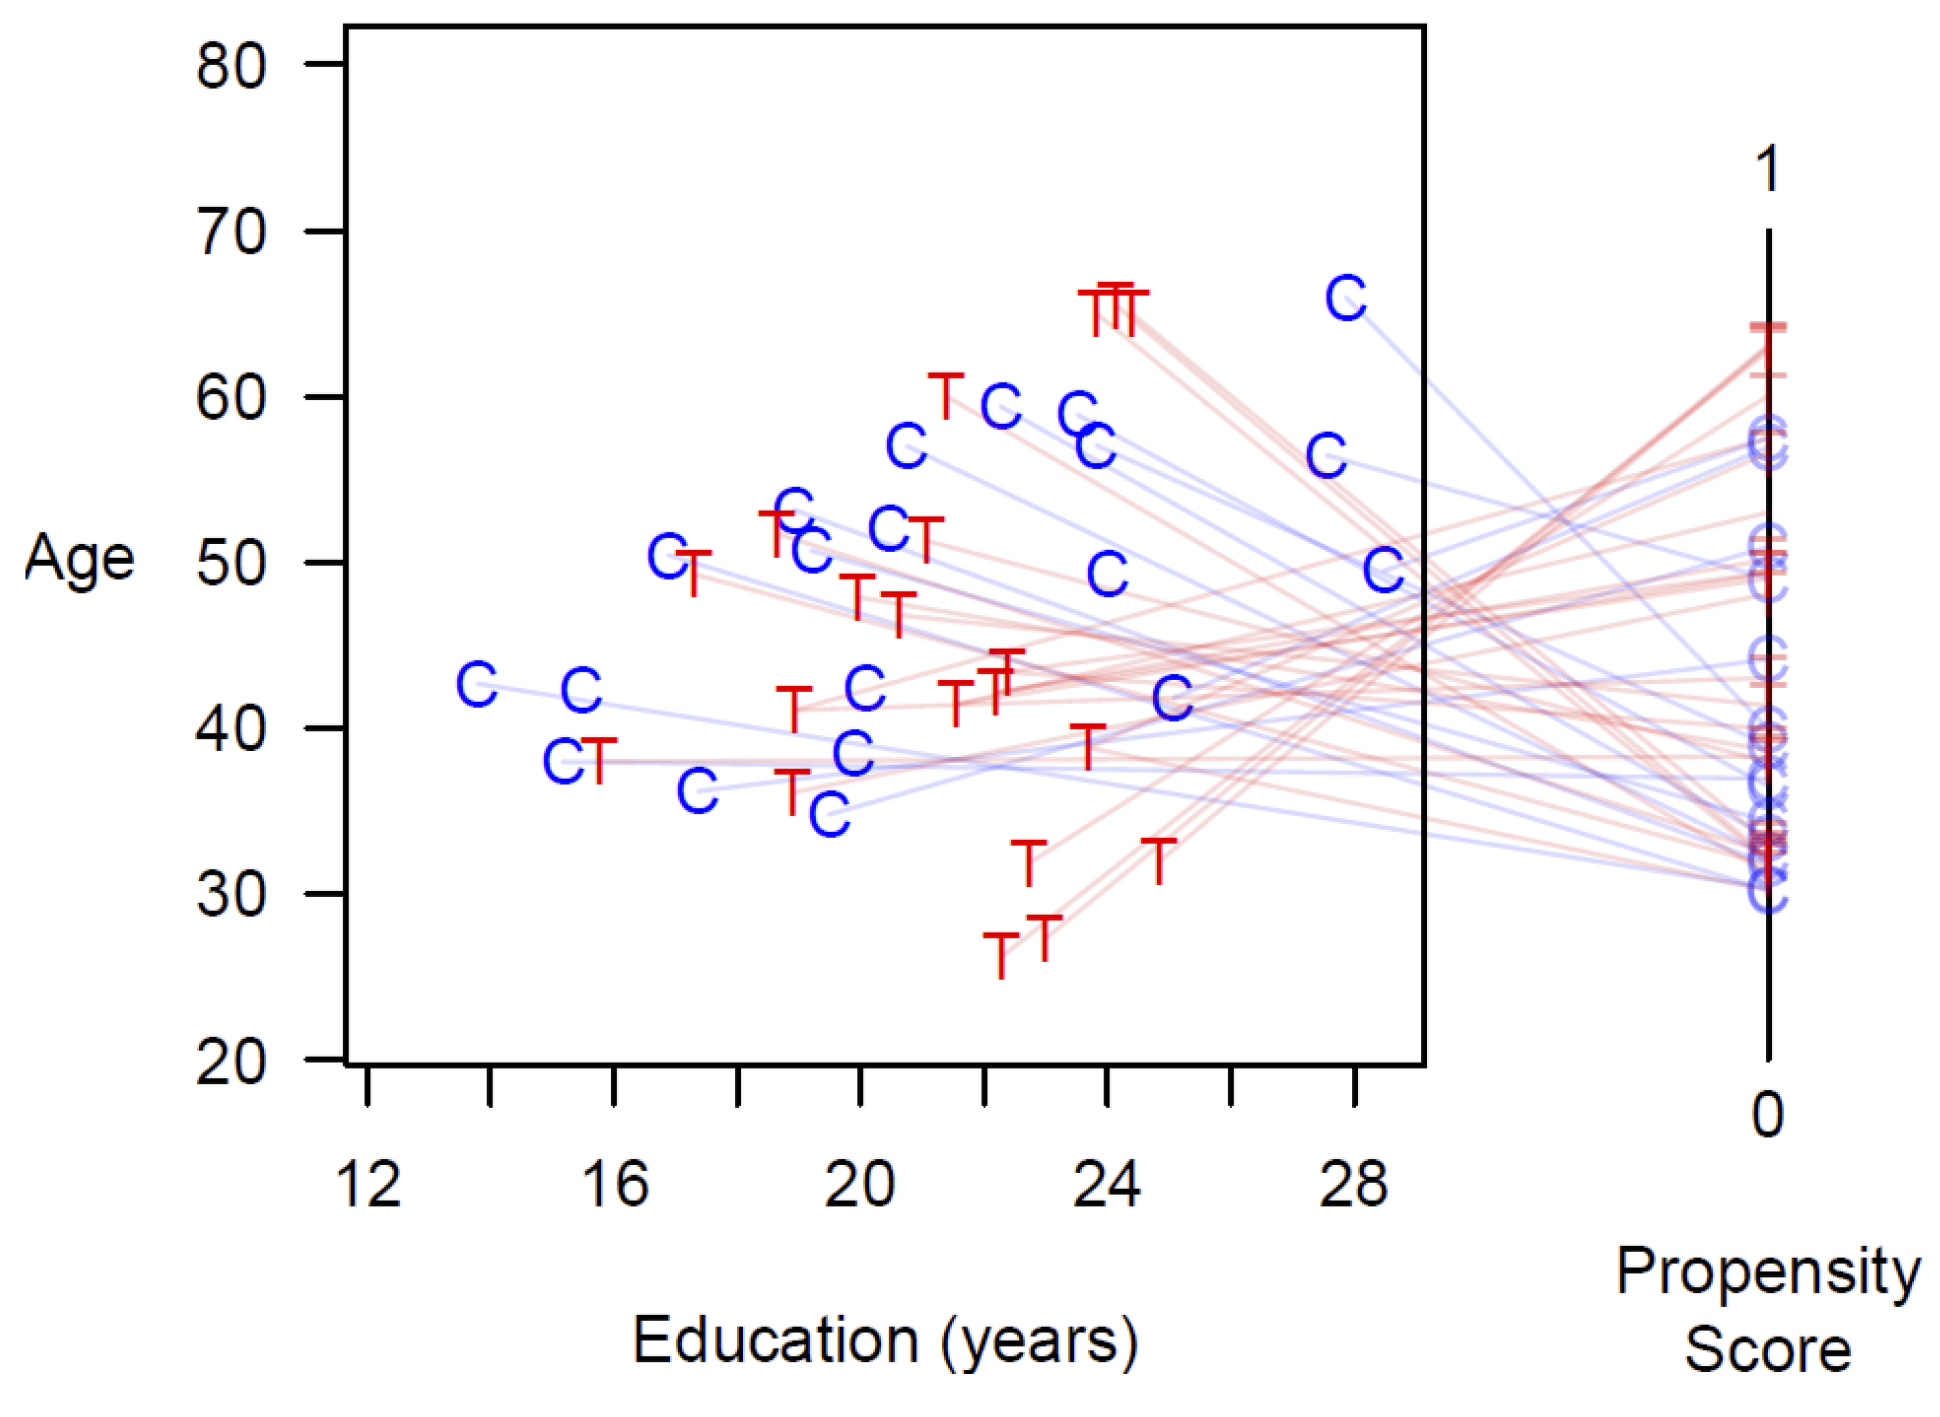
\includegraphics[width=0.7\textwidth]{figure/psm_f5.png}
		\end{figure}
		\begin{minipage}{0.9\linewidth}
			\fontsize{8}{8pt}\selectfont
			\emph{Source:} Ben Elsner's slides
		\end{minipage}
	\end{center}
\end{frame}


\title[]  
{Propensity Score Matching \\ Statistical Inference}

\author 
{}

\institute{}

\date
{}

\begin{frame}{}
	\titlepage
\end{frame}


\begin{frame}{Propensity Score Matching}{Statistical Inference}
	\begin{itemize}
		
		\item A valid method to calculate standard errors has not been known until very recently (see, Abadie and Imbens, 2016)
		\vspace{0.2cm}
			\item Abadie, Alberto, and Guido W. Imbens. ``\textbf{Matching on the Estimated Propensity Score}." Econometrica 84.2 (2016): 781-807.
		\vspace{0.2cm}
		\begin{itemize}		
		
			\item Need to take into account that propensity scores are estimated
			\vspace{0.2cm}
			\item The adjustment for ATE is always negative: smaller standard errors	
			\vspace{0.2cm}
			\item The adjustment for ATT can be positive or negative: smaller or larger standard errors				
		\end{itemize}		
	\end{itemize}
\end{frame}


\begin{frame}{Propensity Score Matching}{Statistical Inference}
	\begin{itemize}
		
		\item A valid method to calculate standard errors when using estimated propensity scores was formally derived by Abadie and Imbens (2016)
		\vspace{0.2cm}
		\item Abadie, Alberto, and Guido W. Imbens. ``\textbf{Matching on the Estimated Propensity Score}." Econometrica 84.2 (2016): 781-807.
		\vspace{0.2cm}
		\begin{itemize}		
			
			\item Need to account for the fact that propensity scores are estimated rather than known
			\vspace{0.2cm}
					\begin{itemize}		
			\item For ATE: The adjustment is always negative, leading to smaller standard errors compared to using true propensity scores
			\vspace{0.2cm}
			\item For ATT: The adjustment can be either positive or negative, leading to either smaller or larger standard errors				
			\vspace{0.2cm}
					\end{itemize}		
			\item Ignoring this adjustment can lead to incorrect inference
		\end{itemize}		
	\end{itemize}
\end{frame}


\begin{frame}{Propensity Score Matching}{Drawback}
	\begin{itemize}
		\item  PSM is hugely popular method to estimate treatment effects even if it relies on \textbf{less convincing assumption}: 
		\vspace{0.2cm}
		\begin{itemize}
			\item Selection on observables (CIA) 	
		\end{itemize}
	\end{itemize}	
\end{frame}


\title[]  
{STATA Example}

\author 
{}

\institute{}

\date
{}

\begin{frame}{}
	\titlepage
\end{frame}


\begin{frame}{STATA Example}{Dehejia et al. (1999)}	Rajeev H. Dehejia; Sadek Wahba (1999)``\textbf{Causal Effects in Nonexperimental Studies: Reevaluating the Evaluation of Training Programs}"Journal of the American Statistical Association 
	\begin{itemize}
		\vspace{0.2cm}
		\item The authors wants to examine the effect of job training on workers' earnings
		\vspace{0.2cm}
		\item We use this example to go through the procedure of implementing PSM
	\end{itemize}
\end{frame}


\begin{frame}{STATA Example}{Dehejia et al. (1999)}
	\begin{itemize}
		\item See \textbf{matching.do}
		\vspace{0.2cm}
		\item Use lalonde.dta
		\vspace{0.2cm}
		\item Install the following ado files:
		\begin{itemize}
			\vspace{0.2cm}
			\item psmatch2.ado 
		\end{itemize}
		
	\end{itemize}
\end{frame}


\begin{frame}[fragile]{Path Setup}{}
\begin{lstlisting}
if "`c(username)'" == "ttyang" {
global do = "C:\nest\Dropbox\causal_data_course\code\Class_Data\do"
global rawdata = "C:\nest\Dropbox\causal_data_course\code\Class_Data\rawdata"
global workdata = "C:\nest\Dropbox\causal_data_course\code\Class_Data\workdata"
}
if "`c(username)'" == "nest" {
global do = "D:\nest\Dropbox\causal_data_course\code\Class_Data\do"
global rawdata = "D:\nest\Dropbox\causal_data_course\code\Class_Data\rawdata"
global workdata = "D:\nest\Dropbox\causal_data_course\code\Class_Data\workdata"
}
\end{lstlisting}
\end{frame}


\begin{frame}[fragile]{Install Package (ado file)}{\texttt{ssc install}}
\begin{lstlisting}
ssc install psmatch2
\end{lstlisting}
	\begin{itemize}
		\vspace{0.2cm}
        \item Install the \texttt{psmatch2} package using the \texttt{ssc install} command
	\end{itemize}
\end{frame}


\begin{frame}[fragile]{Read Data}{import delimited: reads CSV files}
\begin{lstlisting}
import delimited "$rawdata/lalonde.csv", clear

export delimited using "$rawdata/lalonde.csv", replace
\end{lstlisting}
	
	\begin{itemize}
		\vspace{0.2cm}
		\item \textbf{import delimited:} Standard command for reading CSV files in Stata
		\vspace{0.2cm}
		\item \textbf{export delimited:} Writes data to CSV efficiently, with options for handling column names and delimiters
	\end{itemize}
\end{frame}

\begin{frame}[fragile]{Read Data}{use/save: Work with Stata files}
\begin{lstlisting}
use "$rawdata/lalonde.dta", clear

save "$rawdata/lalonde.dta", replace
\end{lstlisting}
	
	\begin{itemize}
		\vspace{0.2cm}
		\item \textbf{use:} Basic command for reading Stata's `.dta` files
		\vspace{0.2cm}
		\item \textbf{save:} Stores data in Stata's native `.dta` format with specified version compatibility
		\vspace{0.2cm}
	\end{itemize}
\end{frame}


\begin{frame}[fragile]{Examine Data}{\texttt{codebook}: Display Summary Statistics}
\begin{lstlisting}
codebook age educ re78
\end{lstlisting}
\begin{itemize}
	\vspace{0.2cm}
	\item Display detailed information about variables: \texttt{age}, \texttt{educ}, and \texttt{re78}
	\vspace{0.2cm}
	\begin{itemize}
		\item \textbf{codebook}: Provides summary statistics, data type, range, and distribution details
		\vspace{0.2cm}
		\item Useful for initial data exploration and understanding variable characteristics
	\end{itemize}
\end{itemize}
\end{frame}


\begin{frame}[fragile]{Examine Data}{\texttt{sum}: Display Summary Statistics}
\begin{lstlisting}
sum re78, d
\end{lstlisting}
\begin{itemize}
	\vspace{0.2cm}
	\item Display detailed summary statistics for \texttt{re78}
	\vspace{0.2cm}
	\begin{itemize}
		\item \textbf{sum}: Computes summary statistics such as mean, standard deviation, and range
		\vspace{0.2cm}
		\item \textbf{d} option: Provides a more detailed summary, including percentiles and extreme values
		\vspace{0.2cm}
		\item Useful for understanding the distribution and variability of 1978 real earnings
	\end{itemize}
\end{itemize}
\end{frame}


\begin{frame}[fragile]{Examine Data}{\texttt{tab}: Produce a frequency table}
\begin{lstlisting}
tab treat
\end{lstlisting}
	\begin{itemize}
		\vspace{0.2cm}
		\item Display frequency table for the \texttt{treat} variable
		\vspace{0.2cm}
		\begin{itemize}
			\item \textbf{tab}: Shows the count and percentage for each category of the \texttt{treat} variable
			\vspace{0.2cm}
			\item Useful for checking the balance between treatment and control groups in the study
		\end{itemize}
	\end{itemize}
	\end{frame}


\begin{frame}[fragile]{Create Sample for Analysis}{\texttt{gen}: Create New Variables}
\begin{lstlisting}
gen id=_n
\end{lstlisting}
\begin{itemize}
	\vspace{0.2cm}
	\item Generate a new variable \texttt{id} as a unique identifier for each observation
	\vspace{0.2cm}
	\begin{itemize}
		\item \textbf{gen}: Creates new variables in Stata
		\vspace{0.2cm}
		\item \textbf{\_n}: Represents the observation number in the dataset
		\vspace{0.2cm}
		\item Useful for creating a unique ID for each row in the dataset
	\end{itemize}
\end{itemize}
\end{frame}


\begin{frame}[fragile]{Examine Data}{\texttt{duplicates}: Detecting Repeated Observations}
\begin{lstlisting}
duplicates report id
\end{lstlisting}
\begin{itemize}
	\vspace{0.2cm}
	\item Check for duplicate values in the \texttt{id} variable
	\vspace{0.2cm}
	\begin{itemize}
		\item \textbf{duplicates report}: Reports the number of observations and distinct values
		\vspace{0.2cm}
		\item Identifies any duplicate entries in the \texttt{id} variable
		\vspace{0.2cm}
		\item Crucial for ensuring each observation has a unique identifier
	\end{itemize}
\end{itemize}
\end{frame}


\begin{frame}[fragile]{STATA Example}{Step 1: Test Differences in Outcomes in Pre-matching Data}
\begin{lstlisting}
ttest re78, by(treat)
\end{lstlisting}
\begin{itemize}
	\vspace{0.2cm}
	\item Perform a two-sample t-test on the \texttt{re78} variable, grouped by the \texttt{treat} variable
	\vspace{0.2cm}
	\begin{itemize}
		\item \textbf{ttest}: Compares the mean 1978 real earnings (\texttt{re78}) between treatment and control groups
		\vspace{0.2cm}
		\item \textbf{by(treat)}: Specifies that the comparison is made between the two groups defined by \texttt{treat}
		\vspace{0.2cm}
		\item Tests whether the difference in means is statistically significant before matching
	\end{itemize}
\end{itemize}
\end{frame}


\begin{frame}{STATA Example}{Step 1: Test Differences in Outcomes in Pre-matching Data}
	\begin{center}
		\begin{figure}[p]
			\centering
			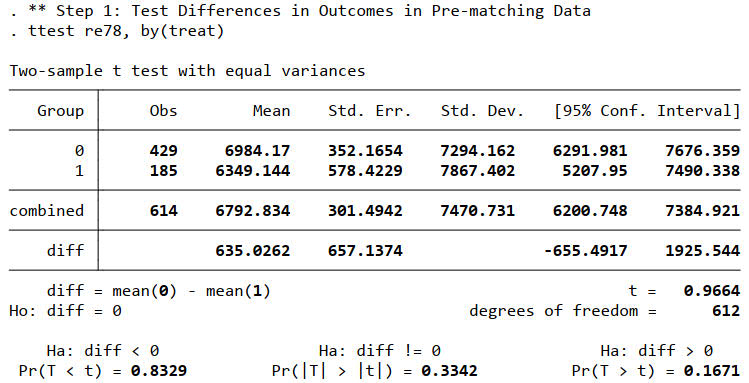
\includegraphics[width=0.9\textwidth]{figure/ttest_1.jpg}
		\end{figure}
	\end{center}
\end{frame}


\begin{frame}[fragile]{STATA Example}{Step 2: Test Differences in Covariates in Pre-matching Data}
\begin{lstlisting}
ttest age, by(treat)
ttest educ, by(treat)
\end{lstlisting}
\begin{itemize}
	\vspace{0.2cm}
	\item Perform two-sample t-tests on the covariates \texttt{age} and \texttt{educ}, grouped by the \texttt{treat} variable
	\vspace{0.2cm}
	\begin{itemize}
		\item \textbf{ttest age, by(treat)}: Compares the mean age between treatment and control groups
		\vspace{0.2cm}
		\item \textbf{ttest educ, by(treat)}: Compares the mean education level between treatment and control groups
		\vspace{0.2cm}
		\item Assesses balance in key covariates before matching to detect pre-existing differences
	\end{itemize}
\end{itemize}
\end{frame}


\begin{frame}{STATA Example}{Step 2: Test Differences in Covariates in Pre-matching Data}
	\begin{center}
		\begin{figure}[p]
			\centering
			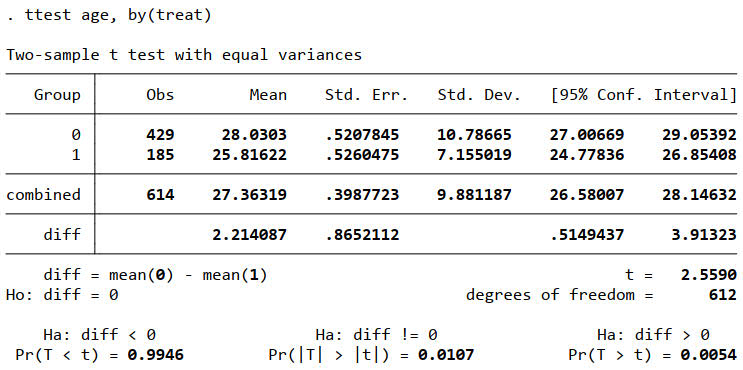
\includegraphics[width=0.9\textwidth]{figure/ttest_2.jpg}
		\end{figure}
	\end{center}
\end{frame}

% FIX #3: \item Syntax: -> \textbf{Syntax:}
\begin{frame}[fragile]{STATA Example}{Step 3: PSM Estimation -- teffects psmatch}
	\textbf{Syntax:}
\begin{lstlisting}
teffects psmatch (outcome) (treatment covariates, logit), nn(#) ate
\end{lstlisting}
	\begin{itemize}
		\vspace{0.2cm}
		\item \textbf{nn($\#$)}: specify number of matches per observation; default is nn(1)
		\vspace{0.2cm}
			\begin{itemize}
		\item The number of variables generated may be more than nn($\#$) because of tied distances
			\end{itemize}
		\vspace{0.2cm}
		\item \textbf{logit}: use logit to predict propensity score (the default)
		\vspace{0.2cm}
		\item \textbf{ate}: estimate average treatment effect in population (the default)
		\vspace{0.2cm}
		\item \textbf{atet}: estimate average treatment effect on the treated  
		
	\end{itemize}
\end{frame}


% FIX #4: \item Example: -> \textbf{Example:}
\begin{frame}[fragile]{STATA Example}{Step 3: PSM Estimation -- teffects psmatch}
	\textbf{Example:}
\begin{lstlisting}
teffects psmatch (re78) (treat age educ  black  hispan  nodegree  married  re74  re75, logit), nn(1) atet
teffects psmatch (re78) (treat age educ  black  hispan  nodegree  married  re74  re75, logit), nn(1) ate
\end{lstlisting}
	\begin{itemize}
		\vspace{0.2cm}
		\item Outcome: \texttt{re78} (earnings in 1978)
		\vspace{0.2cm}
		\item Treatment: \texttt{treat} (get job training or not)
	\end{itemize}
\end{frame}


\begin{frame}{STATA Example}{Step 3: PSM Estimation -- teffects psmatch}
	\begin{center}
		\begin{figure}[p]
			\centering
			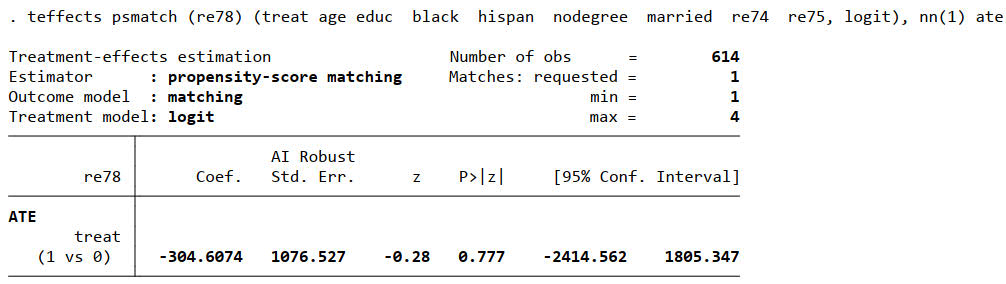
\includegraphics[width=1.0\textwidth]{figure/teffects_1.jpg}
		\end{figure}
	\end{center}
\end{frame}


\begin{frame}{STATA Example}{Step 3: PSM Estimation -- teffects psmatch}
	\begin{center}
		\begin{figure}[p]
			\centering
			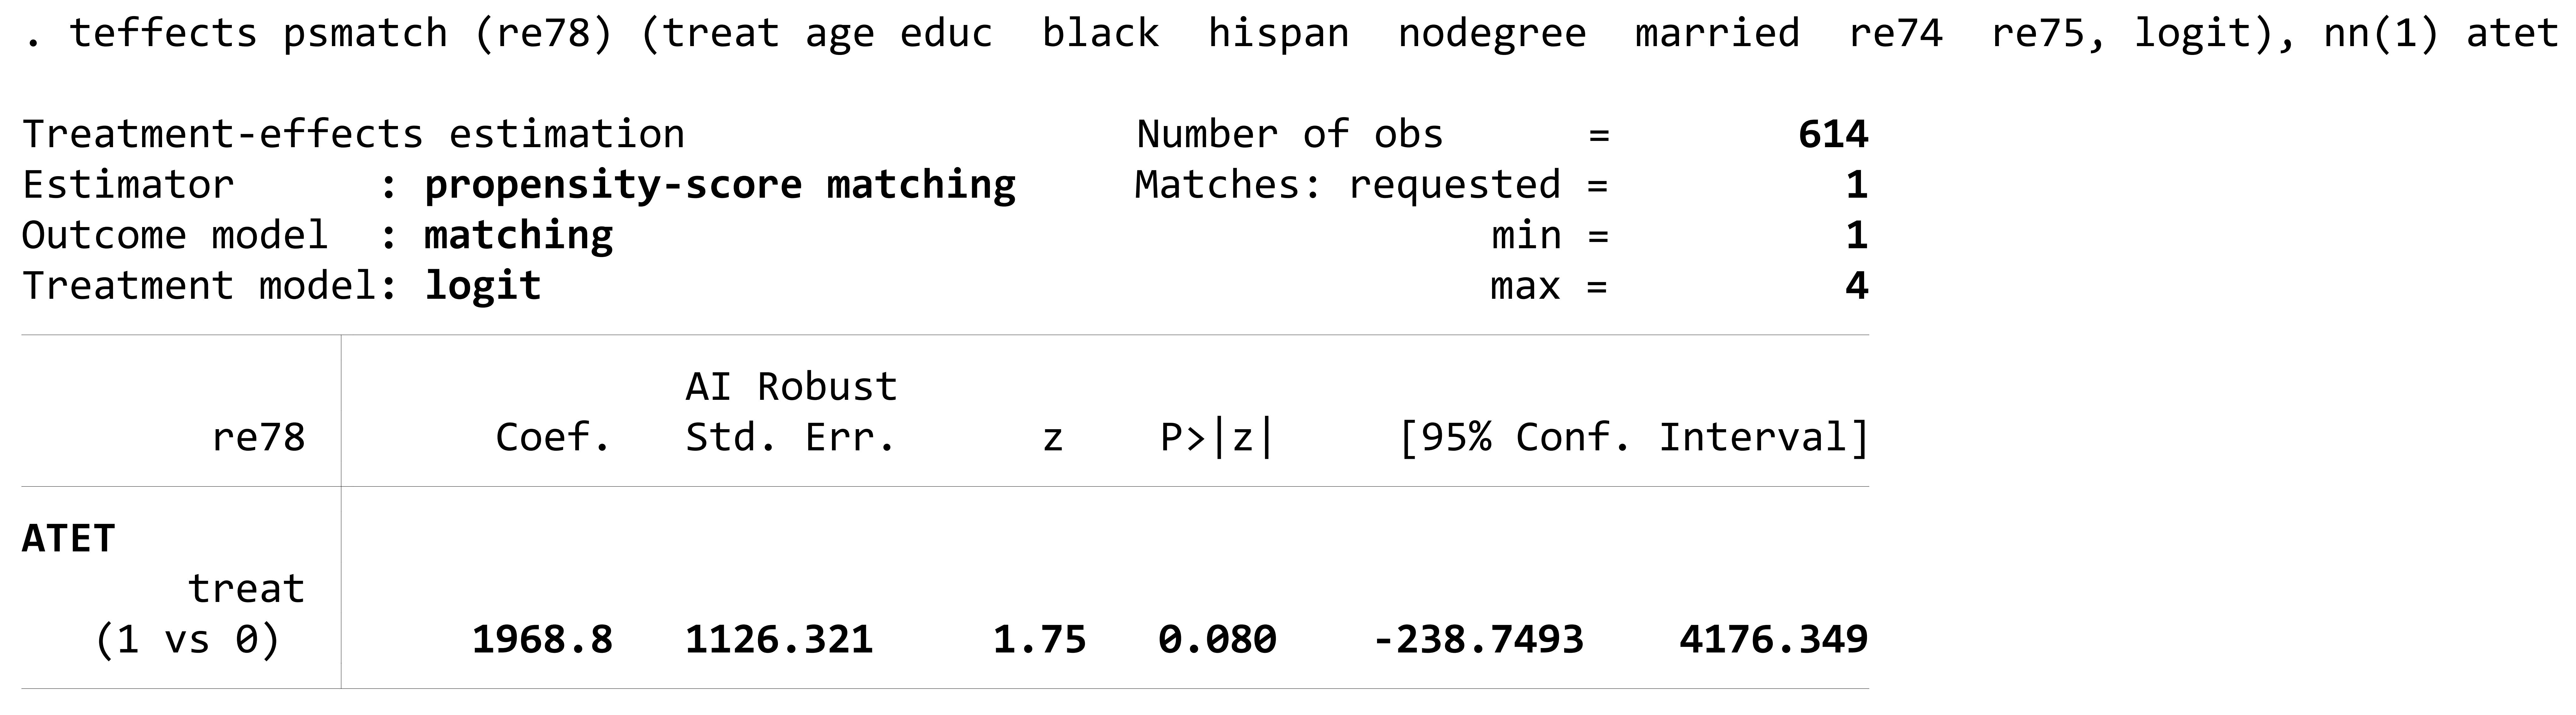
\includegraphics[width=1.0\textwidth]{figure/tteffects_f1_2.jpg}
		\end{figure}
	\end{center}
\end{frame}


% FIX #5: \item Understanding the matching process: -> \textbf{...}
\begin{frame}[fragile]{STATA Example}{Step 3: PSM Estimation -- teffects psmatch}
	\textbf{Understanding the matching process:}
\begin{lstlisting}
teffects psmatch (re78) (treat age educ  black  hispan  nodegree  married  re74  re75), nn(1)  atet gen(matchnum)
\end{lstlisting}
	\begin{itemize}
	\vspace{0.2cm}
	\item \textbf{gen(matchnum)}: specifies that the observation numbers of the nearest neighbors be stored in the new variables matchnum1, matchnum2, ....
		\vspace{0.2cm}
		\item This option is required if you wish to perform postestimation based on the matching results
	\end{itemize}
\end{frame}


% FIX #6: \item Understanding the matching process: -> \textbf{...}
\begin{frame}[fragile]{STATA Example}{Step 3: PSM Estimation -- teffects psmatch}
	\textbf{Understanding the matching process:}
\begin{lstlisting}
predict ps1, ps
predict y0 y1, po
predict te
\end{lstlisting}
	\begin{itemize}
		\vspace{0.2cm}
		\item \textbf{predict ps1, ps}: predict propensity score (i.e. probability of getting treatment)
		\vspace{0.2cm}
		\item \textbf{predict y0 y1, po}: generate the potential outcome with or without treatment
			\vspace{0.2cm}
		\item \textbf{predict te}: get treatment effect for each observation
	\end{itemize}
\end{frame}


\begin{frame}{STATA Example}{Step 3: PSM Estimation -- teffects psmatch}
	\begin{center}
		\begin{figure}[p]
			\centering
			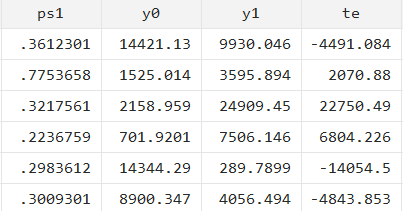
\includegraphics[width=0.82\textwidth]{figure/teffects_data_1.png}
		\end{figure}
	\end{center}
\end{frame}


\begin{frame}{STATA Example}{Step 3: PSM Estimation -- teffects psmatch}
	\begin{center}
		\begin{figure}[p]
			\centering
			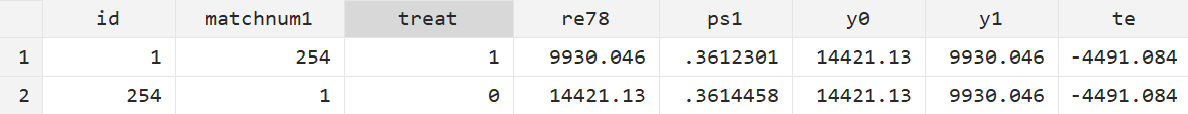
\includegraphics[width=0.82\textwidth]{figure/teffects_data_2.png}
		\end{figure}
	\end{center}
\end{frame}


% FIX #7: \item Syntax: -> \textbf{Syntax:}
\begin{frame}[fragile]{STATA Example}{Step 3: PSM Estimation -- psmatch2}
	\textbf{Syntax:}
\begin{lstlisting}
psmatch2 treatment covariates, out(outcome) n(#) logit ate
\end{lstlisting}
	\begin{itemize}
		\vspace{0.2cm}
		\item \textbf{n($\#$)}: specify number of matches per observation; default is nn(1)
		\vspace{0.2cm}
			\begin{itemize}
		\item The number of variables generated may be more than n($\#$) because of tied distances
			\end{itemize}
		\vspace{0.2cm}
		\item \textbf{out(var)}: specify an outcome variable
		\vspace{0.2cm}
		\item \textbf{ate}: display ATT, ATU, ATE
		
	\end{itemize}
\end{frame}


% FIX #8: \item Example: -> \textbf{Example:}
\begin{frame}[fragile]{STATA Example}{Step 3: PSM Estimation -- psmatch2}
	\textbf{Example:}
\begin{lstlisting}
psmatch2 treat age educ  black  hispan  nodegree  married  re74  re75, out(re78) logit n(1) ate
\end{lstlisting}
	\begin{itemize}
		\vspace{0.2cm}
		\item The PSM estimate is similar to the one using teffects
	\end{itemize}
\end{frame}


\begin{frame}[fragile]{STATA Example}{Compare teffects psmatch and psmatch2}
	\begin{itemize}
		\item The \textbf{teffects psmatch} command has one very important advantage over \textbf{psmatch2}
				\vspace{0.2cm}
			\begin{itemize}		
				\item \textbf{teffects psmatch} takes into account the fact that propensity scores are estimated rather than known when calculating standard errors.
								\vspace{0.2cm}
				\item \textbf{teffects psmatch} calculates standard errors based on this paper:
												\vspace{0.2cm}
							\begin{itemize}		
\item Abadie, Alberto, and Guido W. Imbens. ``\textbf{Matching on the Estimated Propensity Score}." Econometrica 84.2 (2016): 781-807.
								\end{itemize}	
				
				\end{itemize}	
	\end{itemize}
\end{frame}


\begin{frame}[fragile]{STATA Example}{Compare teffects psmatch and psmatch2}
	\begin{itemize}
		\item But \textbf{psmatch2} can allow matching without replacement, which is quite useful. 
	\end{itemize}
\end{frame}


% FIX #9: \item Example: -> \textbf{Example:}
\begin{frame}[fragile]{STATA Example}{Step 3: PSM Estimation -- psmatch2}
	\textbf{Example:}
\begin{lstlisting}
psmatch2 treat age educ  black  hispan  nodegree  married  re74  re75, out(re78) logit n(1) noreplace
\end{lstlisting}
	\begin{itemize}
		\vspace{0.2cm}
		\item \textbf{noreplace}: STATA will perform PSM without replacement so that each untreated observation can be used only once.
	\end{itemize}
\end{frame}


% FIX #10: \item Example: -> \textbf{Example:}
\begin{frame}[fragile]{STATA Example}{Step 4: Post Matching Analysis -- teffects psmatch}
	\textbf{Example:}
\begin{lstlisting}
tebalance box re74
tebalance density educ
tebalance density
\end{lstlisting}
	\begin{itemize}
		\vspace{0.2cm}
		\item \textbf{tebalance box}: Produces box plots that are used to check for balance in
		matched samples after \textbf{teffects}
		
		\vspace{0.2cm}
		\item \textbf{tebalance density}: Produces density plots that are used to check for
		covariate balance after estimation by a \textbf{teffects}
		\vspace{0.2cm}
		\item If you do not specify variable, it will plot the density of propensity score
	\end{itemize}
\end{frame}


\begin{frame}{STATA Example}{Step 4: Post Matching Analysis -- teffects psmatch}
	\begin{center}
		\begin{figure}[p]
			\centering
			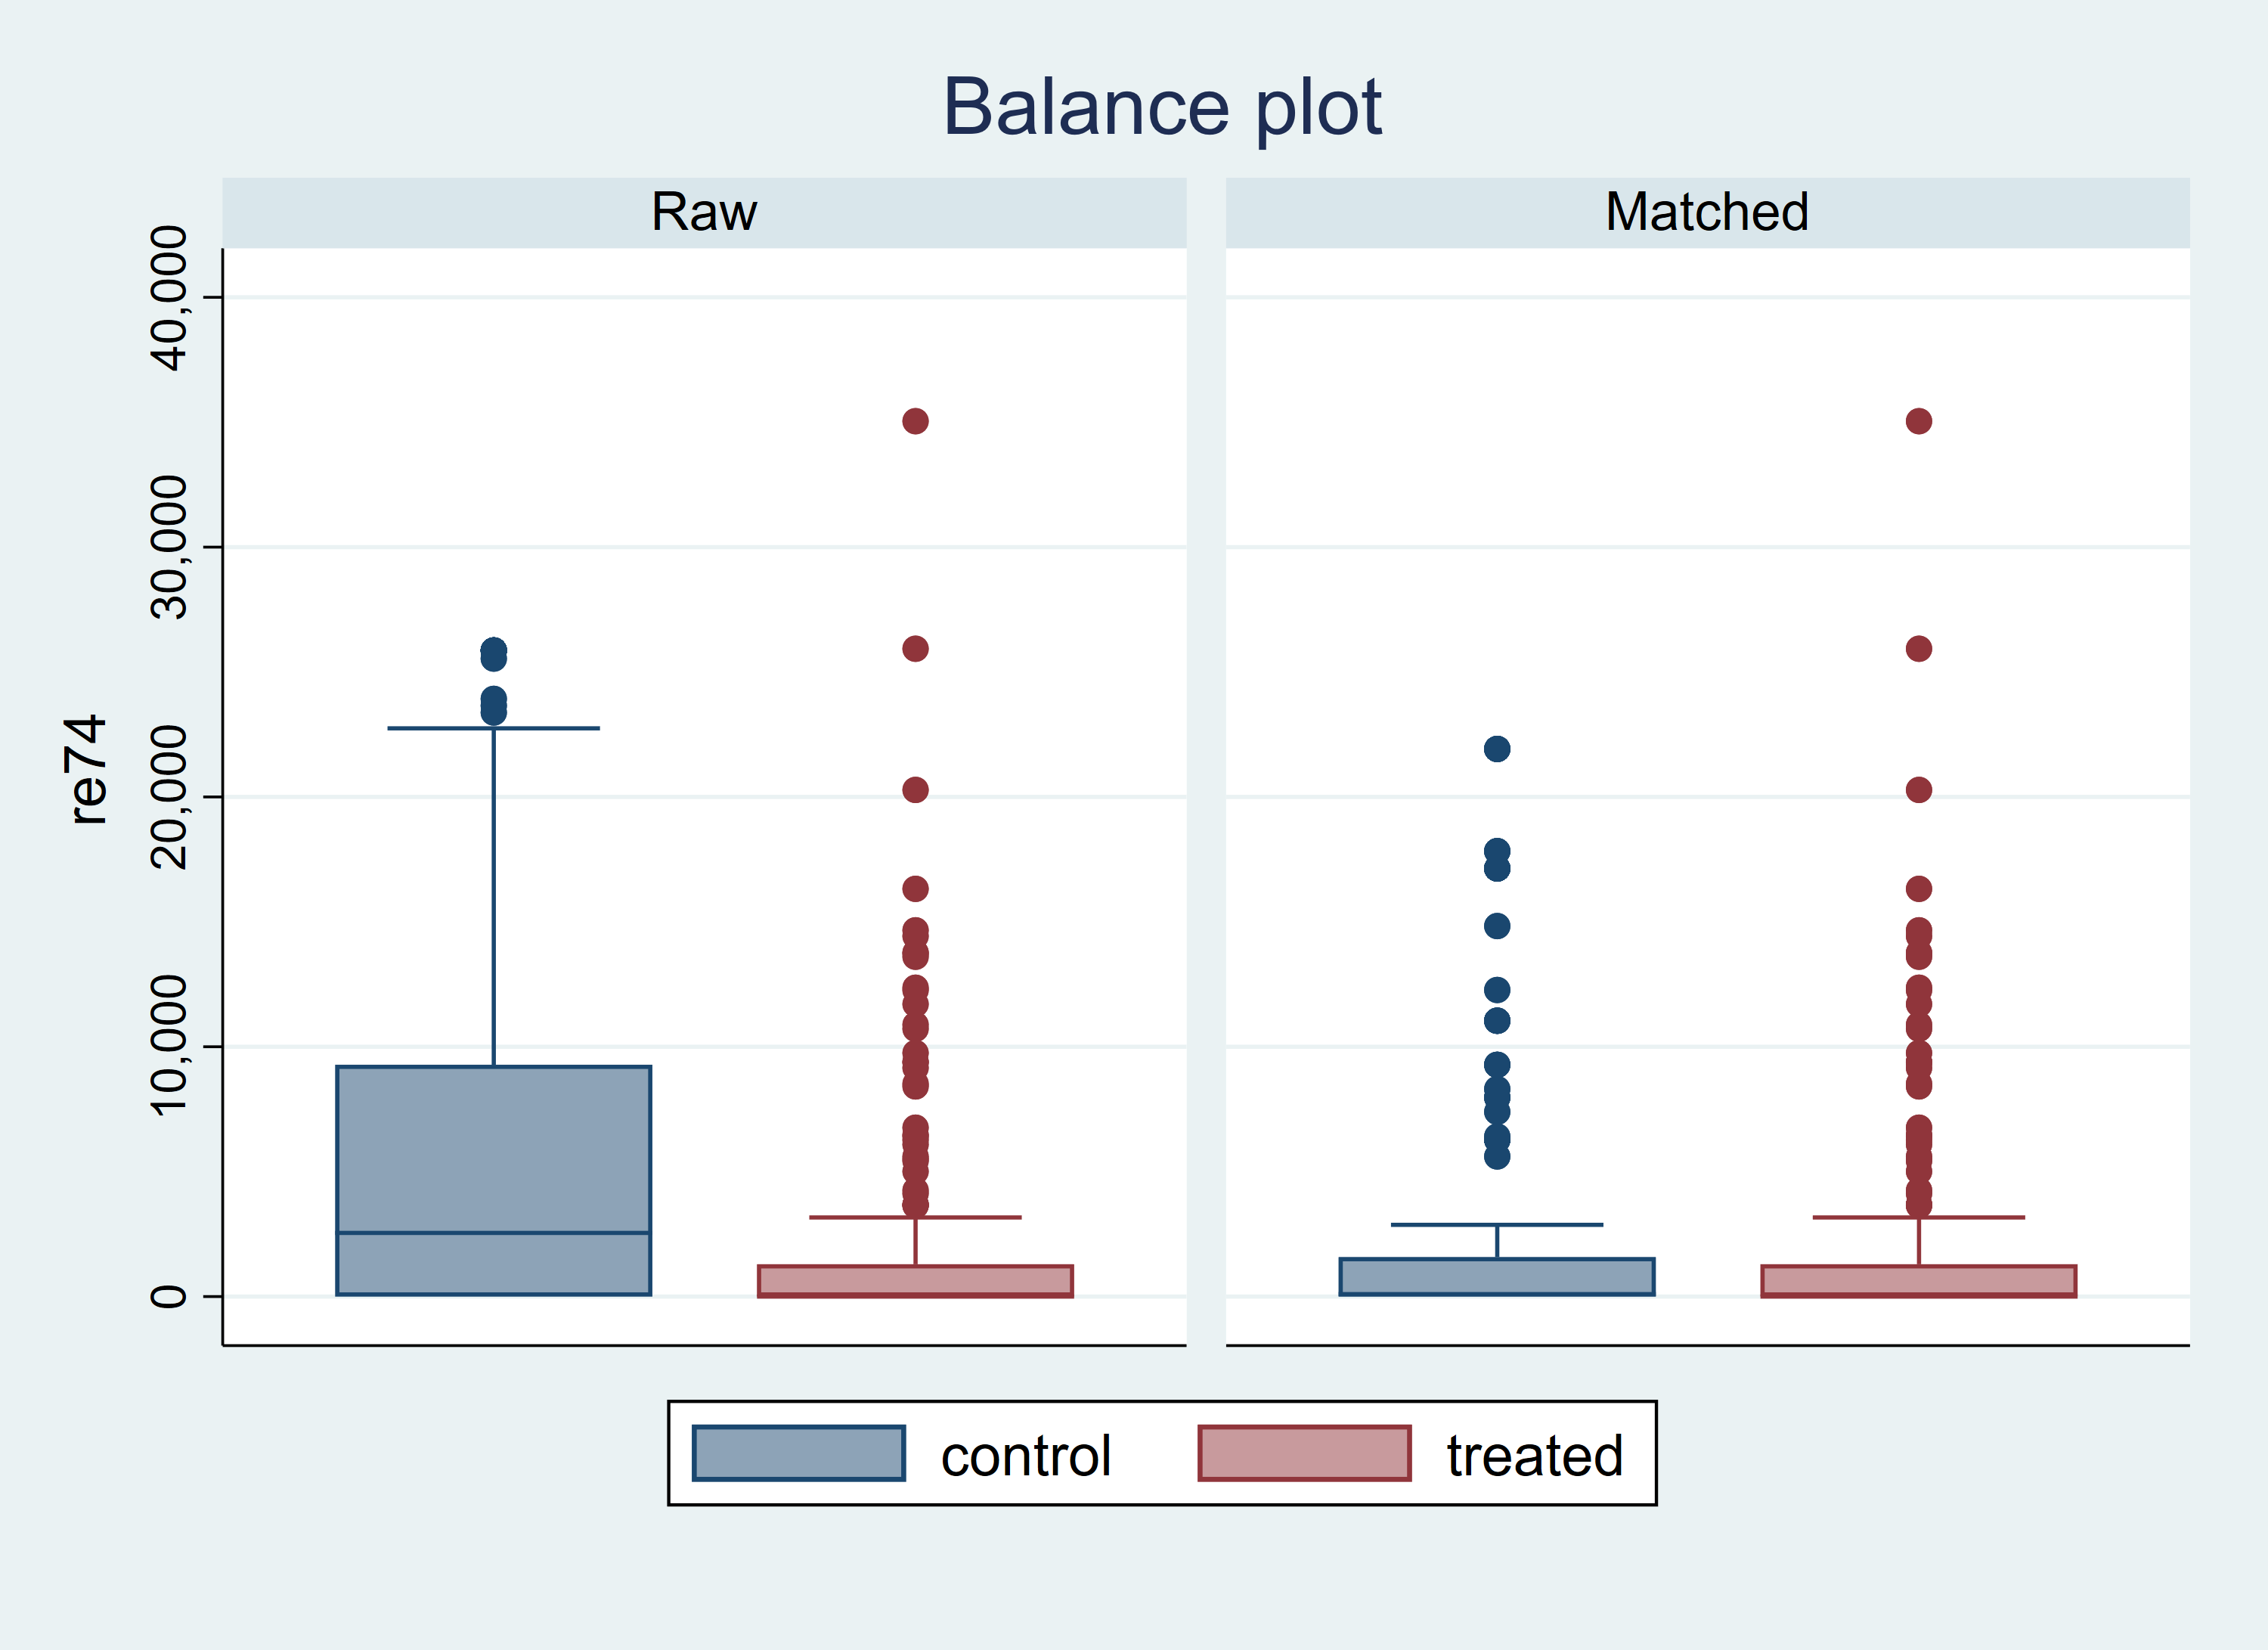
\includegraphics[width=0.9\textwidth]{figure/b-plot.png}
		\end{figure}
	\end{center}
\end{frame}


\begin{frame}{STATA Example}{Step 4: Post Matching Analysis -- teffects psmatch}
	\begin{center}
		\begin{figure}[p]
			\centering
			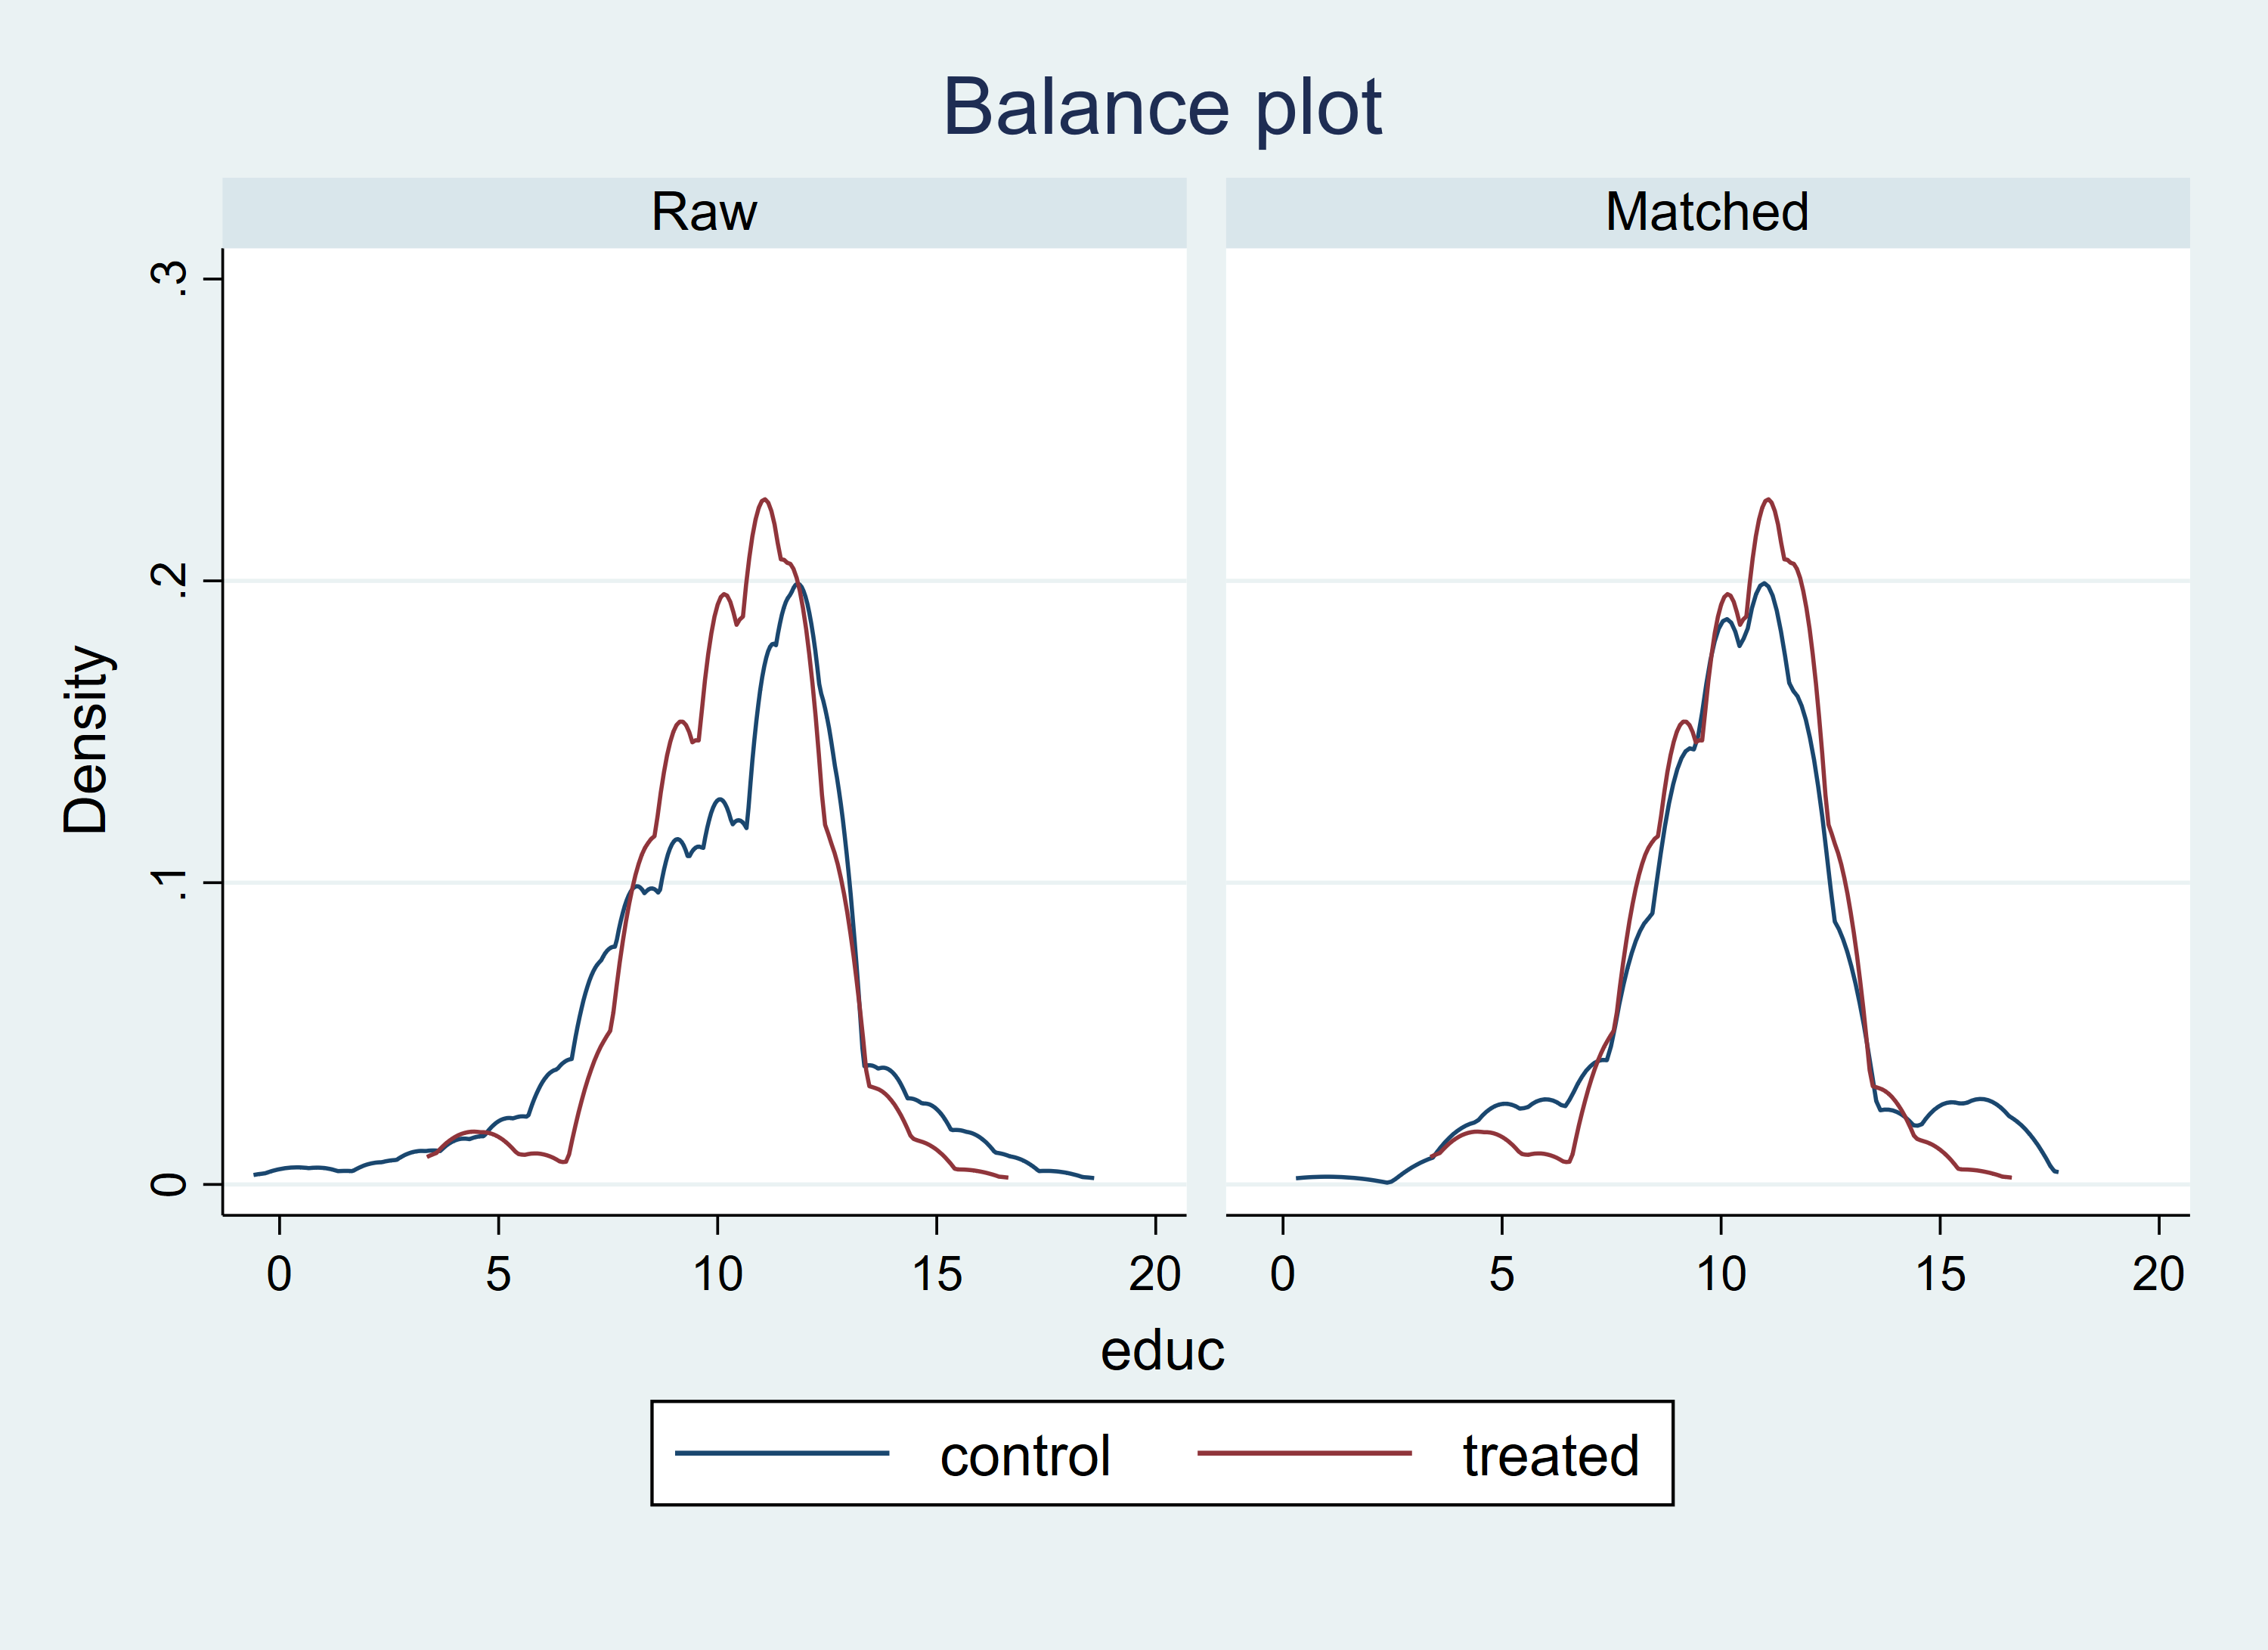
\includegraphics[width=0.9\textwidth]{figure/b-dens.png}
		\end{figure}
	\end{center}
\end{frame}


\begin{frame}{STATA Example}{Step 4: Post Matching Analysis -- teffects psmatch}
	\begin{center}
		\begin{figure}[p]
			\centering
			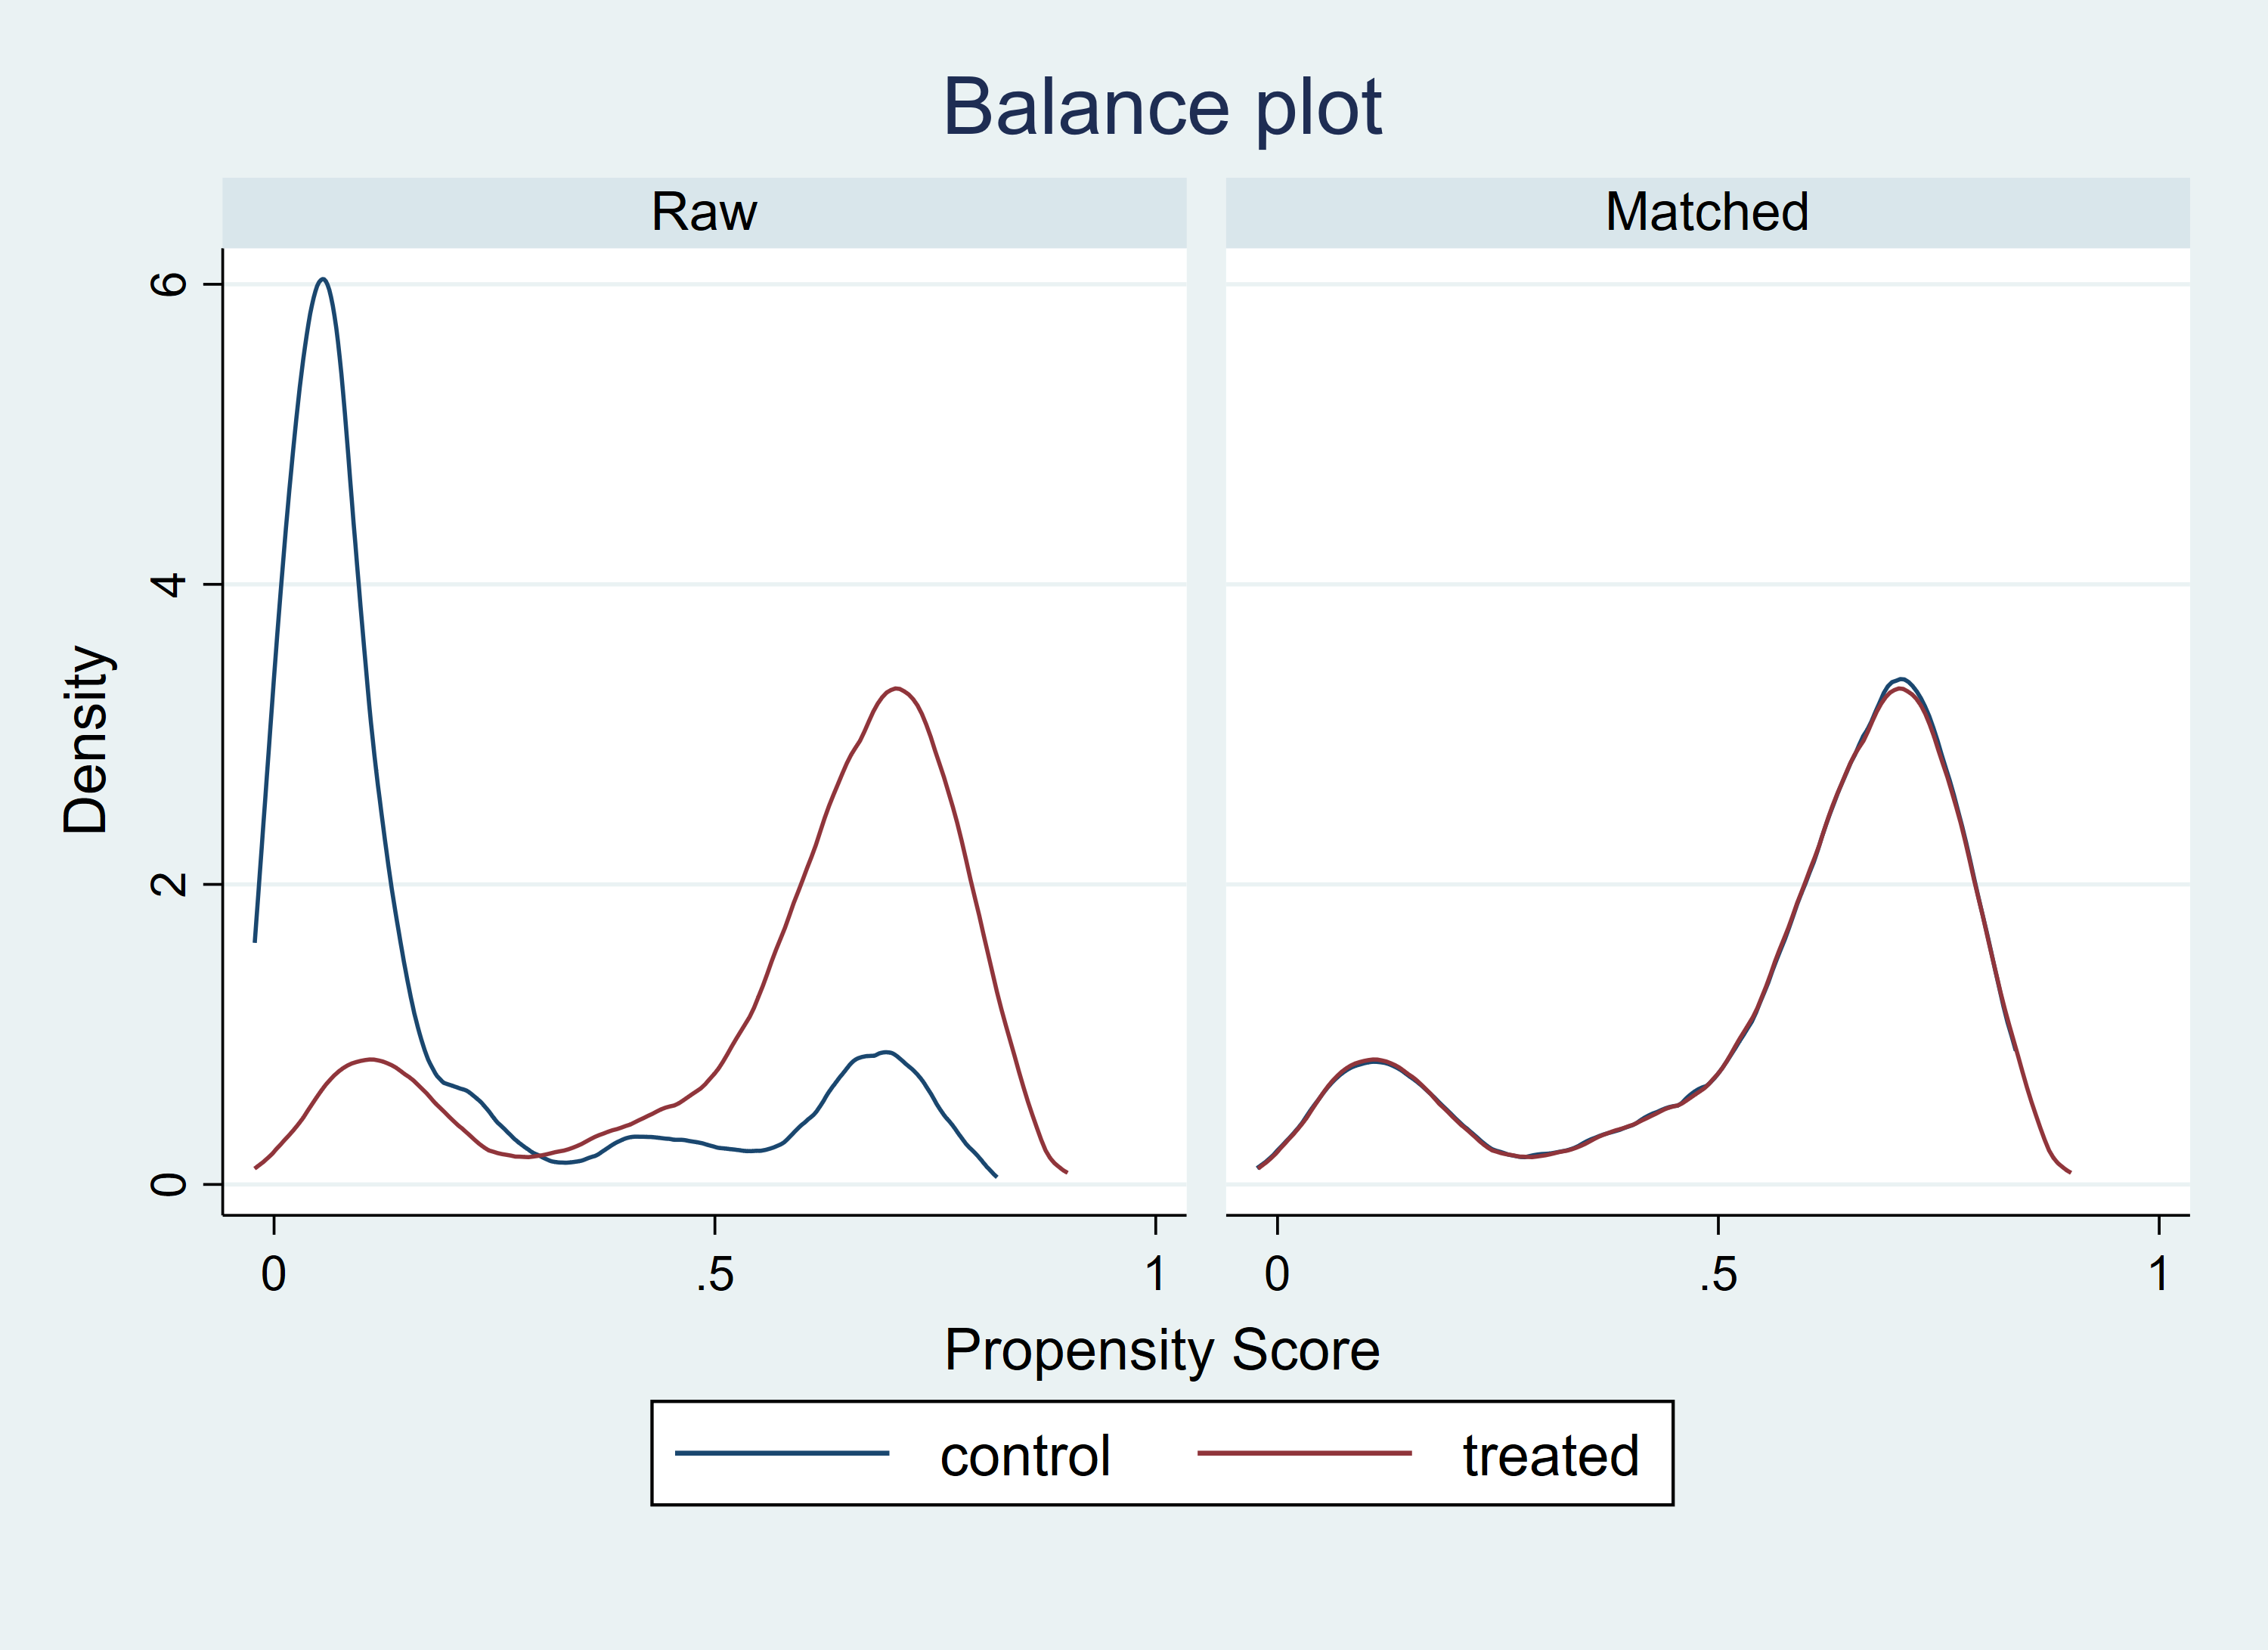
\includegraphics[width=0.9\textwidth]{figure/ps-dens.png}
		\end{figure}
	\end{center}
\end{frame}


% FIX #11: \item Example: -> \textbf{Example:}
\begin{frame}[fragile]{STATA Example}{Step 4: Post Matching Analysis -- psmatch2}
	\textbf{Example:}
\begin{lstlisting}
pstest age educ  black  hispan  nodegree  married  re74  re75, both
pstest educ, box both
pstest _pscore, density both
\end{lstlisting}
	\begin{itemize}
		\vspace{0.2cm}
		\item command \textbf{pstest}: calculates and optionally graphs several measures of the extent of
		balancing of the variables between two groups.
		\vspace{0.2cm}
		\item option \textbf{both}: compares the extent of balancing between the two samples before and after having performed matching.
		\vspace{0.2cm}
		\item option \textbf{box}: draw box plot to compare two groups
		\vspace{0.2cm}
		\item option \textbf{density}: draw density plot to compare two groups
		
	\end{itemize}
\end{frame}


\begin{frame}[fragile]{STATA Example}{Step 4: Post Matching Analysis -- psmatch2}
	\begin{center}
		\begin{figure}[p]
			\centering
			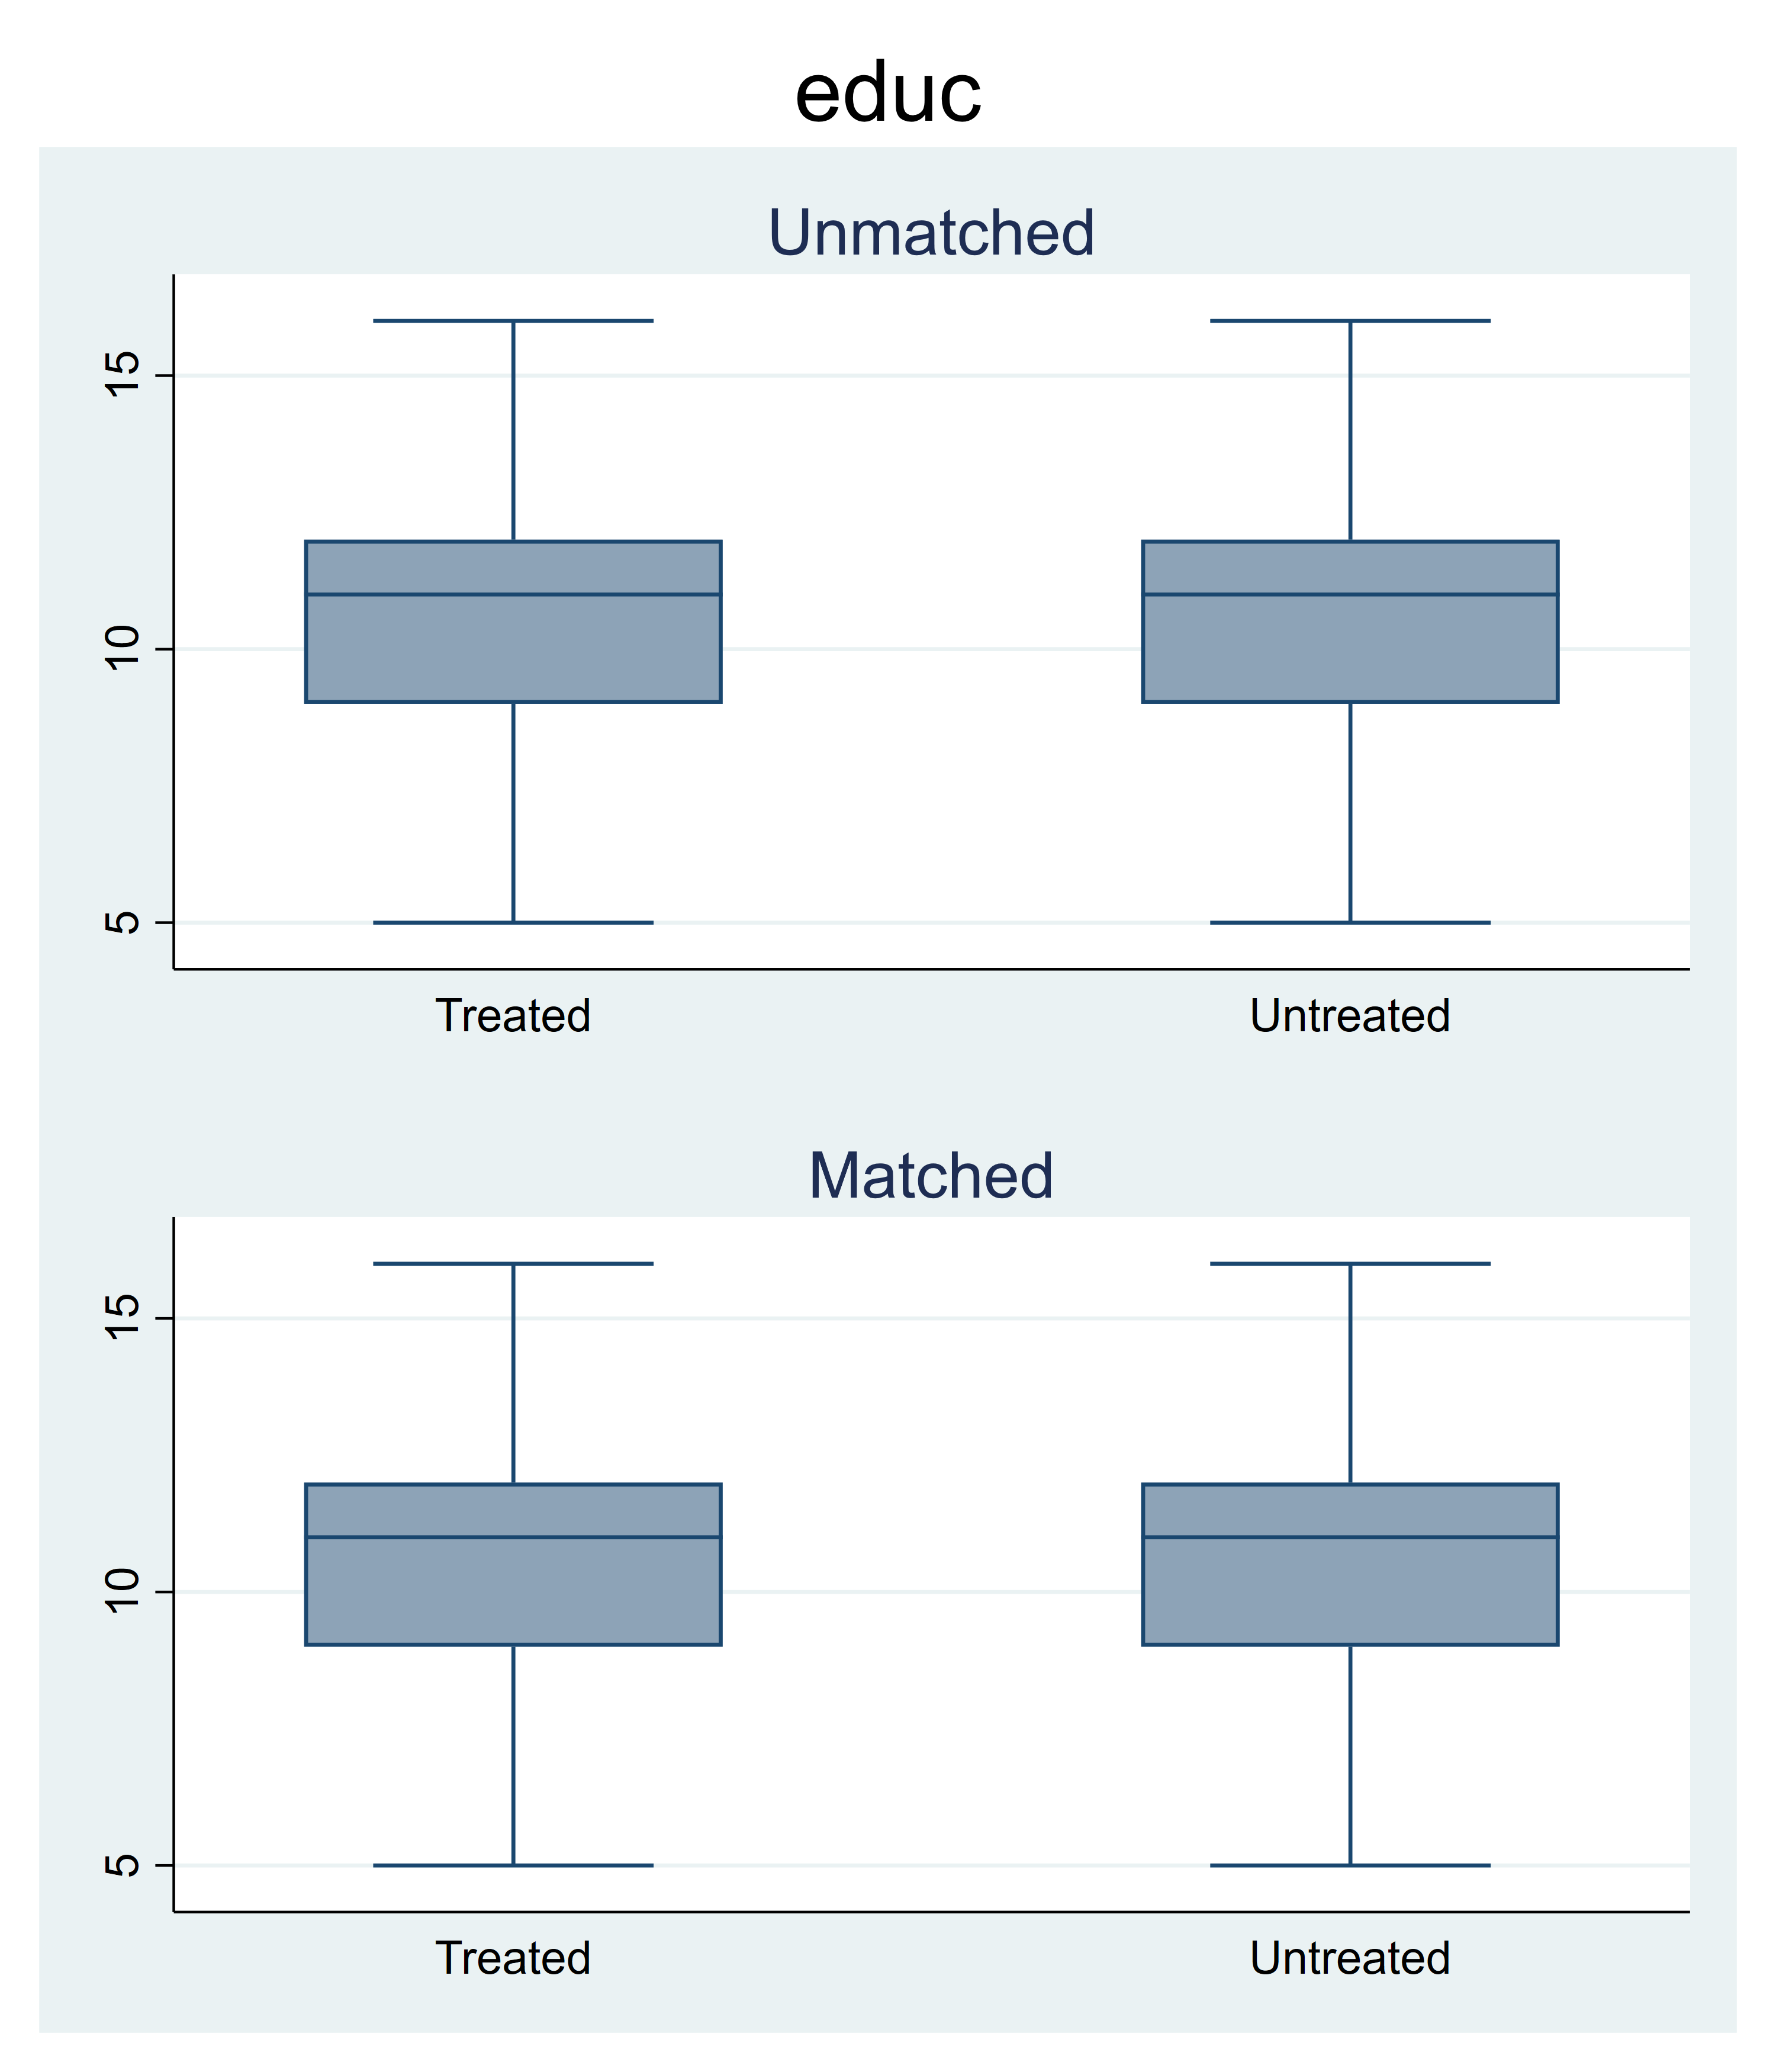
\includegraphics[width=0.5\textwidth]{figure/ps_edu.png}
		\end{figure}
	\end{center}
\end{frame}


\begin{frame}[fragile]{STATA Example}{Step 4: Post Matching Analysis -- psmatch2}
	\begin{center}
		\begin{figure}[p]
			\centering
			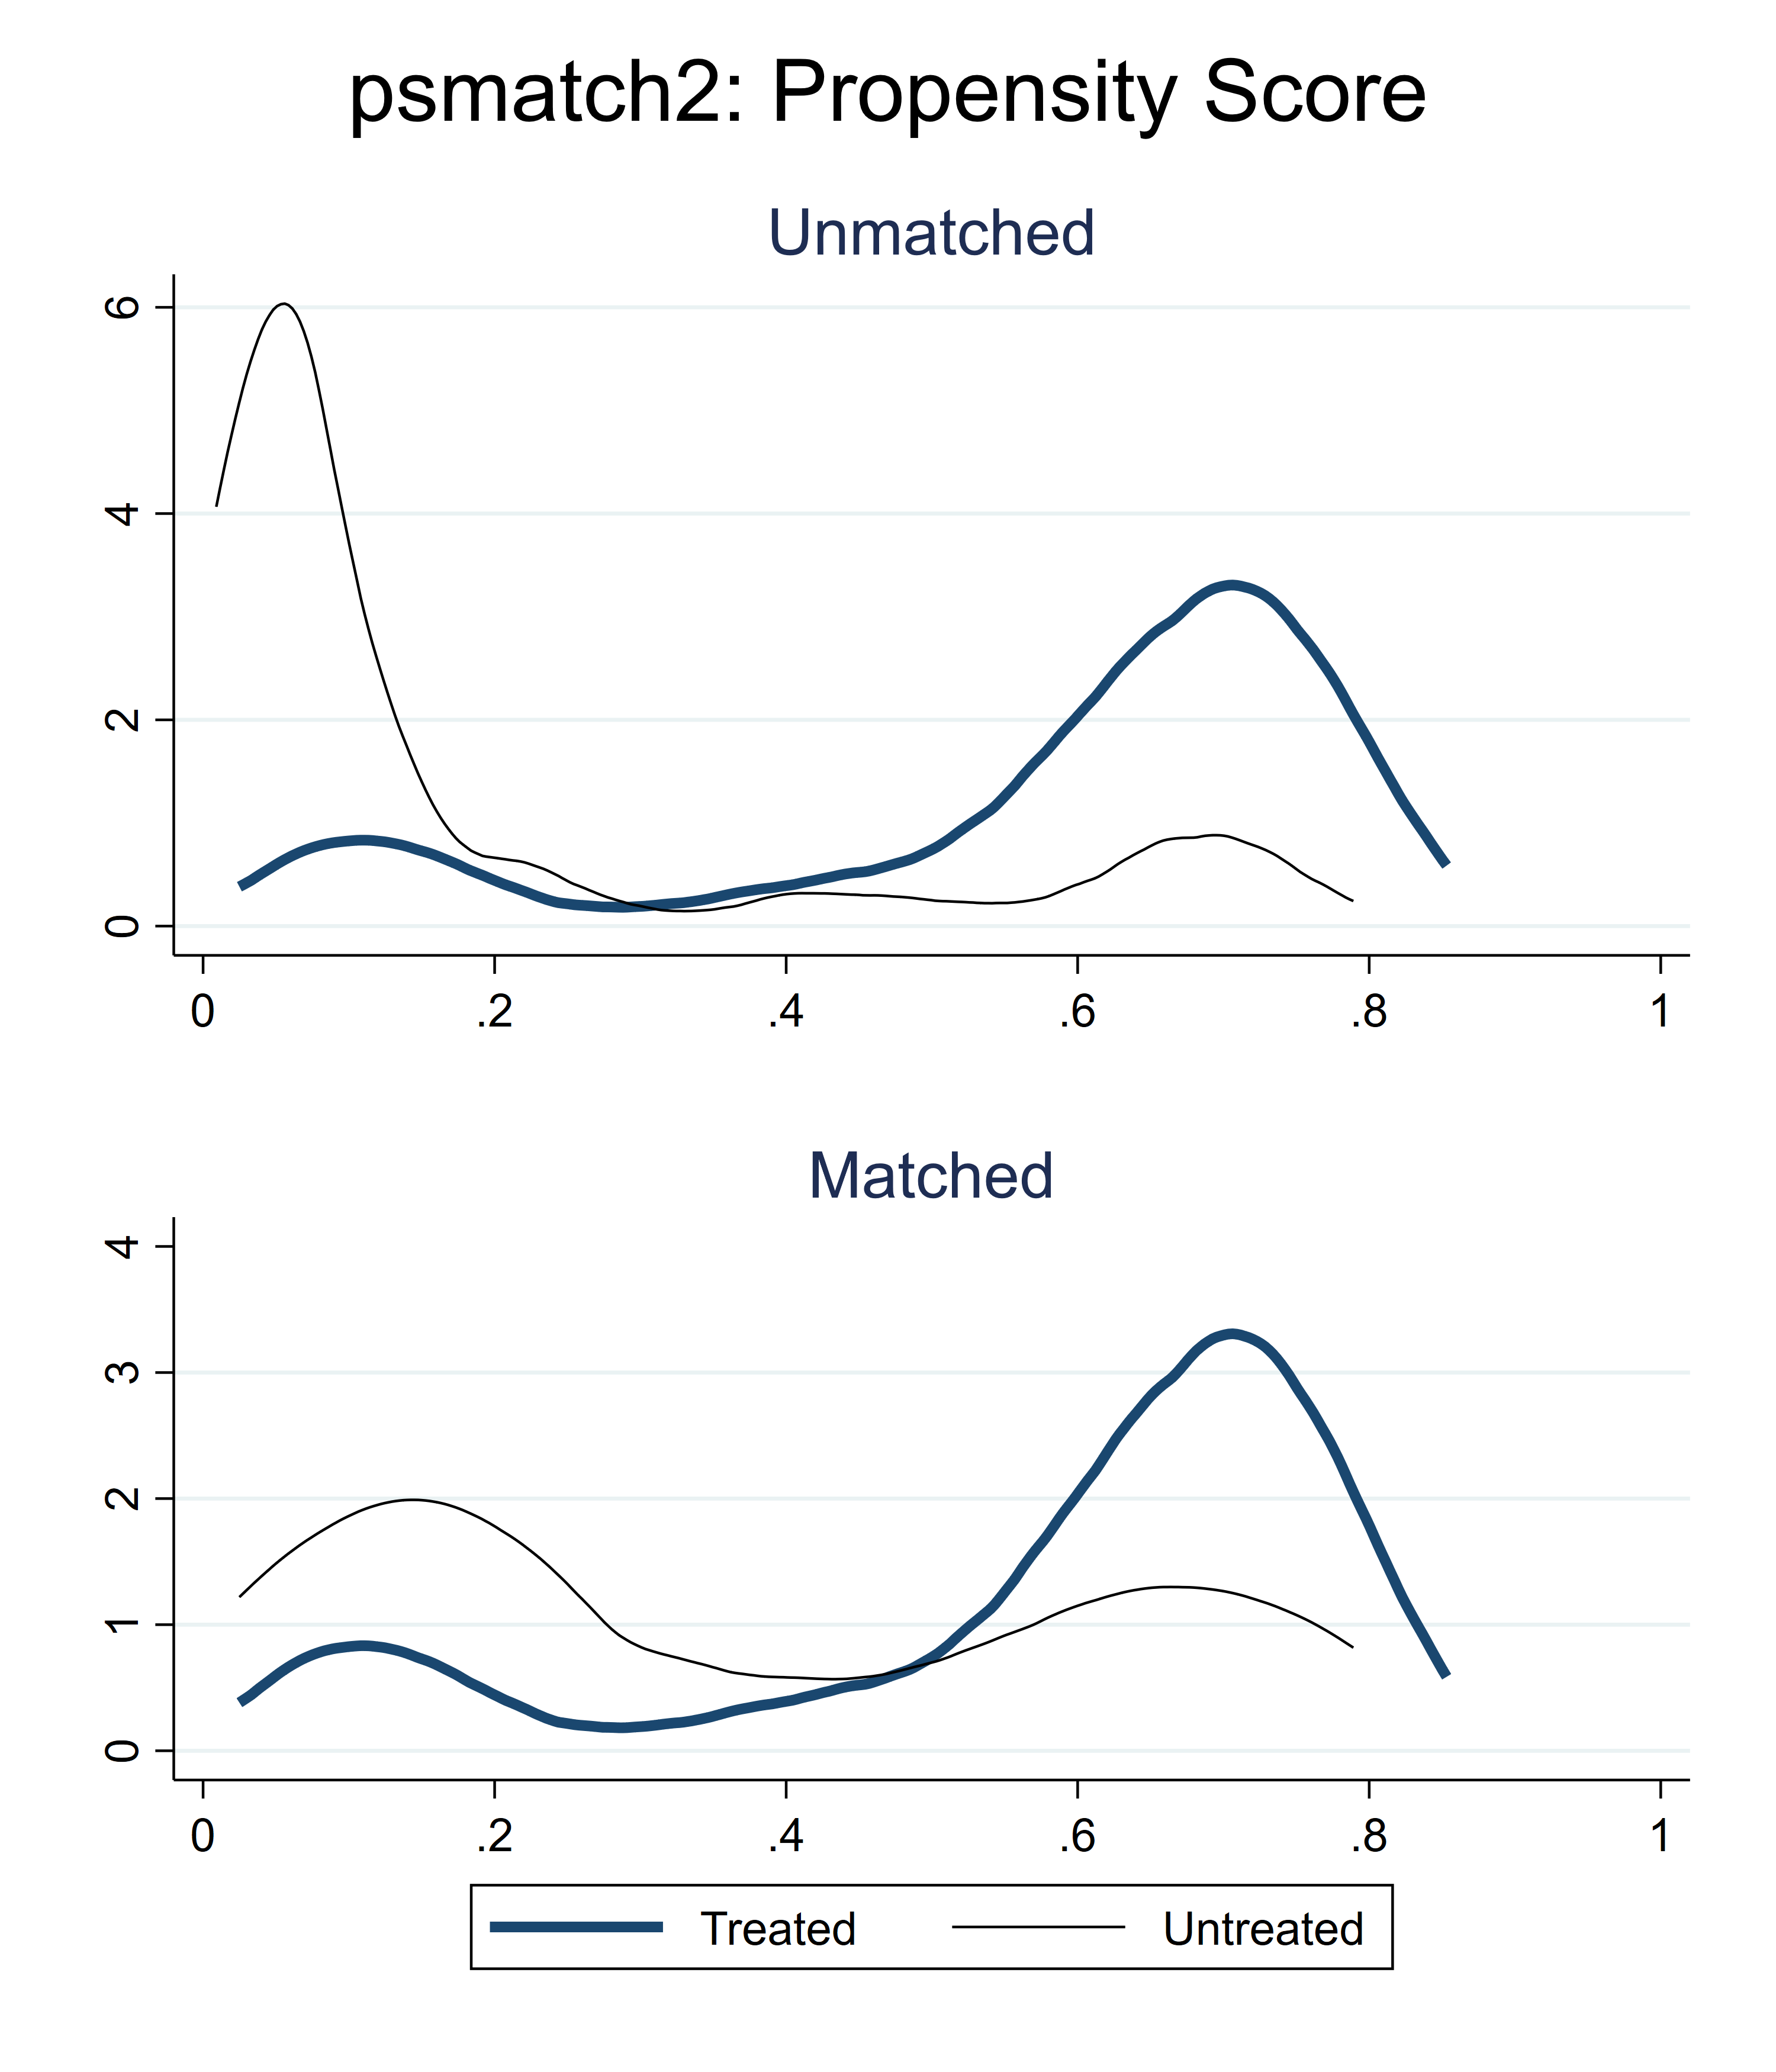
\includegraphics[width=0.5\textwidth]{figure/ps_score.png}
		\end{figure}
	\end{center}
\end{frame}


\title[]  
{R Example}

\author 
{}

\institute{}

\date
{}

\begin{frame}{}
	\titlepage
\end{frame}


\begin{frame}{R Example}{Dehejia et al. (1999)}
	\begin{itemize}
		\item See \textbf{matching.R}
		\vspace{0.2cm}
		\item Use lalonde.dta
		\vspace{0.2cm}
		\item Install the following package:
		\begin{itemize}
			\vspace{0.2cm}
			\item Matching 
		\end{itemize}
		
	\end{itemize}
\end{frame}


\begin{frame}[fragile]{Path Setup}{}
\begin{lstlisting}
rm(list = ls())

# Set paths based on the username
username <- Sys.info()[["user"]]
if (username == "ttyang") {
rawdata <- "C:/nest/Dropbox/causal_data_course/code/Class_Data/rawdata"
} else if (username == "nest") {
 rawdata <- "D:/nest/Dropbox/causal_data_course/code/Class_Data/rawdata"
}
\end{lstlisting}
	\begin{itemize}
		\vspace{0.2cm}
		\item \textbf{rm(list = ls()):} clears all objects from the environment
		\vspace{0.2cm}
		\item \textbf{Sys.info()[["user"]]:} retrieves current system username
		\vspace{0.2cm}
		\item Conditional path setting allows for reproducible workflow across different machines
		\vspace{0.2cm}
		\item Organizes project into logical directories (raw data, working data)
	\end{itemize}
\end{frame}


\begin{frame}[fragile]{Install and Load Package}{\texttt{install.packages()}}
\begin{lstlisting}
# Install necessary packages
install.packages('Matching') # for PSM
install.packages('haven') # for read_dta
install.packages('dplyr') # for mutate 
install.packages('data.table') # for fread


# Load packages
library(Matching) 
library(haven)
library(dplyr)
library(data.table)
\end{lstlisting}
	\begin{itemize}
		\vspace{0.2cm}
			\item \textbf{install.packages()}: downloads and installs the package from CRAN
			\vspace{0.2cm}
			\item \textbf{library()}: loads the installed package for use in the current R session
		\end{itemize}
\end{frame}


\begin{frame}[fragile]{Read Data}{fread(): reads CSV files}
\begin{lstlisting}
lalonde_csv <- fread(paste0(rawdata, "/lalonde.csv"), data.table = FALSE)

fwrite(lalonde, file = paste0(rawdata, "/lalonde.csv"))
\end{lstlisting}
	
	\begin{itemize}
		\vspace{0.2cm}
		\item \textbf{fread:} Efficiently reads CSV files, significantly faster than `read.csv`
		\vspace{0.2cm}
		\item \textbf{fwrite:} Writes data to CSV efficiently, preferred over `write.csv` for large datasets
	\end{itemize}
\end{frame}


\begin{frame}[fragile]{Read Data}{read\_dta(): Read the Stata files}
\begin{lstlisting}
lalonde <- read_dta(paste0(rawdata, "/lalonde.dta"))

write_dta(lalonde_csv, paste0(rawdata, "/lalonde.dta"), version = 14)
\end{lstlisting}
	
	\begin{itemize}
		\vspace{0.2cm}
			\item \textbf{read\_dta:} Reads Stata's `.dta` file into R as a data frame
					\vspace{0.2cm}
		\item \textbf{write\_dta:} Saves data to Stata's `.dta` format with specified version compatibility
		\vspace{0.2cm}
	\end{itemize}
\end{frame}


\begin{frame}[fragile]{Examine Data}{\texttt{summary()}: Display Summary Statistics}
\begin{lstlisting}
summary(lalonde$re78)
\end{lstlisting}
\begin{itemize}
	\vspace{0.2cm}
	\item \textbf{summary():} Provides a concise statistical summary of \texttt{re78}
	\vspace{0.2cm}
	\item Includes:
	\begin{itemize}
		\item Minimum and maximum values
		\vspace{0.2cm}
		\item 1st quartile (25th percentile) and 3rd quartile (75th percentile)
		\vspace{0.2cm}
		\item Median (50th percentile) and mean
	\end{itemize}
	\vspace{0.2cm}
	\item Helps identify potential outliers or skewness in the dataset
\end{itemize}
\end{frame}


\begin{frame}[fragile]{Examine Data}{\texttt{table()}: Display Frequency and Percentage Tables}
\begin{lstlisting}
# Frequency table
table(lalonde$treat)

# Percentage table
prop.table(table(lalonde$treat)) * 100
\end{lstlisting}
\begin{itemize}
	\vspace{0.2cm}
	\item Display frequency and percentage tables for the \texttt{treat} variable
	\vspace{0.2cm}
	\begin{itemize}
		\item \textbf{table():} Shows the count for each category
		\vspace{0.2cm}
		\item \textbf{prop.table()} combined with \textbf{table()} calculates the percentage for each category
	\end{itemize}
\end{itemize}
\end{frame}


\begin{frame}[fragile]{Create Sample for Analysis}{\texttt{mutate()}: Create New Variables}
\begin{lstlisting}
library(dplyr)

lalonde <- lalonde %>%
mutate(id = row_number())
\end{lstlisting}
\begin{itemize}
	\vspace{0.2cm}
	\item \textbf{mutate():} Creates new variables in a data frame
	\vspace{0.2cm}
	\item \textbf{id:} A unique identifier assigned to each observation
	\vspace{0.2cm}
	\begin{itemize}
		\item \textbf{row\_number():} Generates a sequence of numbers based on the current row order
	\end{itemize}
	\vspace{0.2cm}
	\item \textbf{\%>\% (pipe operator):} Passes the left-hand side as the input to the right-hand function
	\vspace{0.2cm}
	\begin{itemize}
		\item Improves readability by avoiding nested function calls
		\vspace{0.2cm}
		\item Allows step-by-step transformations in a logical order
		\vspace{0.2cm}
		\item Commonly used in \texttt{dplyr} for chaining multiple operations
	\end{itemize}
\end{itemize}
\end{frame}


\begin{frame}[fragile]{Examine Data}{\texttt{any(duplicated())}: Check for Duplicates}
\begin{lstlisting}
# Check for any duplicates
any(duplicated(lalonde$id))

# Count total number of duplicates
sum(duplicated(lalonde$id))
\end{lstlisting}
\begin{itemize}
	\vspace{0.2cm}
	\item \textbf{Checking for Duplicates:} Ensures each observation has a unique identifier
	\vspace{0.2cm}
	\begin{itemize}
		\item \textbf{duplicated()}: Identifies duplicate entries in a vector or column
		\vspace{0.2cm}
		\item \textbf{any(duplicated())}: Returns \texttt{TRUE} if there are any duplicates, otherwise \texttt{FALSE}
		\vspace{0.2cm}
		\item \textbf{sum(duplicated())}: Counts the total number of duplicate entries
	\end{itemize}
	\vspace{0.2cm}
	\item Useful for detecting data entry errors and ensuring data integrity before analysis
\end{itemize}
\end{frame}


\begin{frame}[fragile]{R Example}{Step 1: Test Differences in Outcomes in Pre-matching Data}
\begin{lstlisting}
t.test(re78 ~ treat, data = lalonde)
\end{lstlisting}
\begin{itemize}
	\vspace{0.2cm}
	\item Perform a two-sample t-test on the \texttt{re78} variable, grouped by the \texttt{treat} variable
	\vspace{0.2cm}
	\begin{itemize}
		\item \textbf{t.test()}: Compares the mean 1978 real earnings (\texttt{re78}) between treatment and control groups
		\vspace{0.2cm}
		\item Tests whether the difference in means is statistically significant before matching
	\end{itemize}
\end{itemize}
\end{frame}


\begin{frame}[fragile]{R Example}{Step 2: Test Differences in Covariates in Pre-matching Data}
\begin{lstlisting}
# T-test for age
t.test(age ~ treat, data = lalonde)

# T-test for education
t.test(educ ~ treat, data = lalonde)
\end{lstlisting}
	\begin{itemize}
		\vspace{0.2cm}
		\item Perform two-sample t-tests on the covariates \texttt{age} and \texttt{educ}, grouped by the \texttt{treat} variable
	
	\end{itemize}
\end{frame}


% FIX #12: \item Example: -> \textbf{Example:}
\begin{frame}[fragile]{R Example}{Step 3: PSM Estimation}
	\textbf{Example:}
\begin{lstlisting}
# Estimate propensity scores
ps_model <- glm(treat ~ age + educ + black + hispan + nodegree + married + re74 + re75, 
family = binomial(link = "logit"), 
data = lalonde)

# Extract propensity scores
lalonde$ps <- predict(ps_model, type = "response")
\end{lstlisting}
	\begin{itemize}
		\vspace{0.2cm}
		\item \textbf{glm:} estimate logistic regression for propensity scores
		\vspace{0.2cm}
		\item \textbf{predict(..., type = "response"):} extract probability estimates (propensity scores)
		\vspace{0.2cm}
		\item Manually estimating PS gives more control over the process
	\end{itemize}
\end{frame}

\begin{frame}[fragile]{R Example}{Step 3: PSM Estimation}
\begin{lstlisting}
# Perform nearest neighbor matching (with replacement)
m.out_with_replace <- Match(
Y = lalonde$re78,           # Outcome variable
Tr = lalonde$treat,         # Treatment variable
X = lalonde$ps,             # Propensity score
M = 1,                      # 1:1 matching
replace = TRUE,             # Matching with replacement
estimand = "ATT")           # Average Treatment Effect on Treated

# View results
summary(m.out_with_replace)
\end{lstlisting}
	\begin{itemize}
		\vspace{0.2cm}
		\item \textbf{Match:} performs matching and estimates treatment effect directly
		\vspace{0.2cm}
		\item Uses Abadie \& Imbens variance estimator automatically when matching with replacement
	\end{itemize}
\end{frame}


% ================================================================
% Coarsened Exact Matching (CEM)
% ================================================================

\title[]
{Coarsened Exact Matching \\ (CEM)}

\author
{}

\institute{}

\date
{}

\begin{frame}{}
\titlepage
\end{frame}


\begin{frame}{Coarsened Exact Matching (CEM)}
	\begin{itemize}
		\item PSM reduces matching to one dimension (the propensity score), but requires a correctly specified model
		\vspace{0.2cm}
		\item \textbf{CEM} takes a more direct approach:
		\vspace{0.2cm}
		\begin{itemize}
			\item \textbf{Coarsen} each covariate into discrete bins (e.g., age 20--29, 30--39, \ldots)
			\vspace{0.2cm}
			\item \textbf{Exact match} on the coarsened values: a treated and a control unit are matched only if they fall in the \emph{same bin for every covariate}
			\vspace{0.2cm}
			\item Units with no match in any covariate are \textbf{discarded}
		\end{itemize}
		\vspace{0.2cm}
		\item No propensity score model needed --- covariate balance is \textbf{guaranteed by construction}
	\end{itemize}
\end{frame}


\begin{frame}{How CEM Works}{Steps 1 \& 2: Coarsen and Match}
	\begin{itemize}
		\item[1] \textbf{Coarsen}: bin each continuous covariate $X_k$ into discrete intervals (automatic or user-defined cutpoints)
		\vspace{0.2cm}
		\begin{itemize}
			\item E.g., age: $[20,30)$, $[30,40)$, $[40,50)$; earnings: $[0, 5\text{K})$, $[5\text{K}, 15\text{K})$, \ldots
		\end{itemize}
		\vspace{0.3cm}
		\item[2] \textbf{Exact match} on coarsened values:
		\vspace{0.2cm}
		\begin{itemize}
			\item Two units are matched only if they fall in the \emph{same bin for every covariate}
			\vspace{0.2cm}
			\item Each such group of matched units is called a \textbf{stratum}: think of it as a subgroup of ``similar'' units who share the same coarsened covariate profile
			\vspace{0.2cm}
			\item Units with no match in any covariate are \textbf{discarded}
		\end{itemize}
	\end{itemize}
\end{frame}


\begin{frame}{How CEM Works}{Step 3: Estimate ATT}
	\begin{itemize}
		\item[3] For each treated unit $i$, impute the counterfactual using the \textbf{average outcome of control units in the same stratum} $s(i)$:
	\begin{equation*}
		\hat{\alpha}_{\text{ATT}} = \dfrac{1}{N_1}\sum_{D_i=1}\!\left(Y_i - \bar{Y}_{0,s(i)}\right)
	\end{equation*}
	\begin{itemize}
		\item $N_1$: total number of treated units 
        
        %--- same as before; note $\textstyle\sum_s N_{1,s} = N_1$
		\vspace{0.2cm}
		\item $s(i)$: the stratum that treated unit $i$ belongs to
		\vspace{0.2cm}
		\item $\bar{Y}_{0,s(i)} = \dfrac{1}{N_{0,s(i)}}\!\displaystyle\sum_{D_j=0,\,j\in s(i)}\!Y_j$: average \emph{observed} outcome of control units ($D_j=0$) in $i$'s stratum
		%\vspace{0.15cm}
		%\item Compare with the matching estimator: $\hat{\alpha}_{\text{ATT}}=\frac{1}{N_1}\sum_{D_i=1}(Y_i - Y_{j(i)})$ --- the only difference is $Y_{j(i)}$ is replaced by $\bar{Y}_{0,s(i)}$
        	\end{itemize}
	\end{itemize}
\end{frame}


\begin{frame}{Advantages of CEM}
	\begin{itemize}
		\item \textbf{No model dependence}: no propensity score to estimate, so no misspecification risk
		\vspace{0.2cm}
		\item \textbf{Guaranteed balance}: treated and matched controls share the same covariate bins by construction
		\vspace{0.2cm}
		\item \textbf{Transparent}: the coarsening is explicit and easy to interpret
		\vspace{0.2cm}
		\item \textbf{Tradeoff}: 
		\vspace{0.2cm}

        	\begin{itemize}

        \item Finer bins $\Rightarrow$ better balance but fewer matched units 
        		\vspace{0.2cm}

        \item Coarser bins $\Rightarrow$ more matches but looser balance
        	\end{itemize}

	\end{itemize}
\end{frame}


% ================================================================
% CEM: STATA Example
% ================================================================

\title[]
{CEM: STATA Example}

\author
{}

\institute{}

\date
{}

\begin{frame}{}
\titlepage
\end{frame}


\begin{frame}[fragile]{CEM: Stata Example}{Install Package and Run CEM}
\begin{lstlisting}
use $rawdata\lalonde.dta, replace

* Install cem package
ssc install cem

* Automatic coarsening (Sturges' rule)
cem age educ black hispan nodegree married re74 re75, ///
    treatment(treat)
\end{lstlisting}
	\begin{itemize}
		\vspace{0.2cm}
		\item \textbf{cem varlist, treatment()}: coarsens each variable, exact-matches, and creates \texttt{cem\_weights} and \texttt{cem\_matched}
		\vspace{0.2cm}
		\item Without cutpoints, CEM uses automatic (Sturges' rule) coarsening
	\end{itemize}
\end{frame}


\begin{frame}[fragile]{CEM: Stata Example}{Estimate ATT}
\begin{lstlisting}
* Estimate ATT on matched sample using CEM weights
reg re78 treat [iweight=cem_weights] if cem_matched==1, r

* Optional: manual coarsening (specify number of bins)
cem age (#4) educ (#3) re74 (#5) re75 (#5) ///
    black hispan nodegree married, treatment(treat)

reg re78 treat [iweight=cem_weights] if cem_matched==1, r
\end{lstlisting}
	\begin{itemize}
		\vspace{0.2cm}
		\item \textbf{iweight=cem\_weights}: applies CEM weights to balance strata
		\vspace{0.2cm}
		\item \textbf{\#k}: specifies $k$ equal-width bins for that variable
	\end{itemize}
\end{frame}


% ================================================================
% CEM: R Example
% ================================================================

\title[]
{CEM: R Example}

\author
{}

\institute{}

\date
{}

\begin{frame}{}
\titlepage
\end{frame}


\begin{frame}[fragile]{CEM: R Example}{Run CEM and Estimate ATT}
\begin{lstlisting}
install.packages('cem')
library(cem)

# Run CEM with automatic coarsening
m.cem <- cem(treatment = "treat",
             data      = lalonde,
             drop      = "re78")   # exclude outcome variable
summary(m.cem)

# Estimate ATT via weighted regression on matched sample
est <- att(m.cem, re78 ~ treat, data = lalonde)
summary(est)
\end{lstlisting}
	\begin{itemize}
		\item \textbf{cem()}: coarsens covariates and creates strata; \texttt{drop} excludes the outcome
		\vspace{0.1cm}
		\item \textbf{att()}: estimates ATT using CEM weights
	\end{itemize}
\end{frame}


\begin{frame}{Suggested Readings}
	\begin{itemize}
		\item Chapter 2, Mastering Metrics: The Path from Cause to Effect
		\vspace{0.2cm}
		\item Chapter 3, Mostly Harmless Econometrics
		\vspace{0.2cm}
		\item Chapter 5, Causal Inference: The Mixtape
	\end{itemize}
\end{frame}


\end{document}